\documentclass[a4paper, 10pt, english]{article}
\usepackage[utf8]{inputenc}
\usepackage[total={6.69in, 10in}]{geometry}
\usepackage[english]{babel}
\usepackage{silence}
\WarningFilter{latex}{File `}
\WarningFilter{latex}{Package}
% \newcommand{\sectionbreak}{\clearpage}
\hbadness=10000
\vbadness=10000
\usepackage{microtype}
\usepackage{collcell}
\usepackage{etoolbox}
\usepackage{xstring}
\usepackage{lipsum}
\usepackage{listings}

\usepackage{tikz, ifthen, xstring, calc, pgfopts}
\usepackage{pgf-umlcd}
\usepackage[ruled,linesnumbered]{algorithm2e}
% %\usepackage{algorithm}
% %\usepackage{algpseudocode} %% Algorithms is this ok Roni?
\usepackage{tikz} %%% Plot graphs 
\usetikzlibrary{shapes,decorations,arrows,calc,arrows.meta,fit,positioning}
\usepackage{todonotes}
\usepackage{fancyhdr}
\usepackage{enumerate}
\usepackage[hyphens]{url}
\urlstyle{same}
\usepackage{url}
% \def\UrlBreaks{\do\/\do-}
% \usepackage{breakurl}
\usepackage{blindtext}

\usepackage{pdfpages}
\usepackage{csvsimple}
% \usepackage{subfig}
% \usepackage{subfigure}
\usepackage{bookmark}
\usepackage{setspace}
\usepackage{reledmac}
\usepackage{setspace}
\usepackage{microtype}
% \usepackage{etoolbox}
% \usepackage{etool}
% \usepackage{dblfnote}
% \usepackage{ftnright}
% \arrangementX[A]{twocol}
% % \colalignX{\justifying}
% \makeatletter
% \bhooknoteX[A]{\setstretch{1}}
% \bhookgroupX[A]{\setstretch{1}}
% \makeatother
% \let\footnote\footnoteA
\usepackage{datatool}
% \usepackage[bookmarksnumbered]{hyperref} %add hidelinks evt
\usepackage[capitalise, noabbrev]{cleveref}
\crefdefaultlabelformat{#2\textbf{#1}#3}
\newcounter{RQ}
\renewcommand{\theRQ}{\textbf{\arabic{RQ}}}
\crefname{RQ}{RQ}{RQs}
%\crefformat{RQ1}{\textbf{RQ1}}
%\crefformat{RQ2}{\textbf{RQ2}}
%\crefformat{RQ3}{\textbf{RQ3}}
%\crefformat{RQ4}{\textbf{RQ4}}
\crefname{subsec}{subsection}{subsections}
\Crefname{subsec}{Subsection}{Subsections}
\usepackage{hyperref}

\usepackage{graphicx}
\usepackage{pgf-pie} %%% make pies 
\usepackage{pgfplots} %%% PLOT THAT SHITTS
\usepgfplotslibrary{statistics}
\usepackage{pgfplotstable}
\pgfplotsset{compat=1.14}
\usepackage{wrapfig}
\usepackage[labelfont=bf]{caption}
%\captionsetup[figure]{font=small}
\usepackage{indentfirst}
\usepackage{subcaption}
\graphicspath{ {./Figures/} }
%Table packages
\usepackage{longtable}
\usepackage{amsmath, tabu, centernot}
\newcommand{\bigCI}{\mathrel{\text{\scalebox{1.07}{$\perp\mkern-10mu\perp$}}}}
\newcommand{\nbigCI}{\centernot{\bigCI}}
\usepackage{xcolor,colortbl}
\usepackage[export]{adjustbox}
\usepackage{multirow}
\usepackage{multicol}
\usepackage{float}
\usepackage{changepage} %% indents paragrahs with \adjustwidth 
\usepackage{array}
%table text size
\usepackage{pdfpages}
\usepackage{bbding} %%%% Add icons like checkmars with command: \Checkmark
%%\usepackage{stmaryrd} %%%% Add icons like arrows 
%%\usepackage{mathabx} %%%% Add math icons 
%TOC 
\usepackage{titlesec}
\usepackage[titletoc]{appendix}
% \titleformat{\chapter}[display]
%   {\normalfont\bfseries}{}{10pt}{\Huge\thechapter.\quad}
%Vis sidetal
\usepackage{lastpage}
%font
\usepackage[sc]{mathpazo}
\linespread{1.05} 
% load a colour package
% \usepackage{xcolor}
\definecolor{aaublue}{RGB}{33,26,82}% dark blue
% Make the standard latex tables look so much better
\usepackage{array,booktabs}
% Enable the use of frames around, e.g., theorems
% The framed package is used in the example environment
\usepackage{framed}
% Defines new environments such as equation,
% align and split 
\usepackage{amsmath}
\usepackage{mathtools}
% Adds new math symbols
\usepackage{amssymb}
% Use theorems in your document
% The ntheorem package is also used for the example environment
% When using thmmarks, amsmath must be an option as well. Otherwise \eqref doesn't work anymore.
\usepackage[amsmath,thmmarks]{ntheorem}
%lav afsnit med denne commando
\newcommand{\nytafsnit}{\newline\newline \indent}


\usepackage[giveninits=true, backend = biber, style=nature]{biblatex}
\usepackage{hyphenat}

\bibliography{bib.bib}

\usepackage{csquotes}
\newtheorem{theorem}{Theorem} 
\newtheorem{definition}{Definition}
% \newtheorem{lemma}{Lemma}

\titleformat{\chapter}{}{}{0em}{\bfseries\LARGE\ifnum\value{chapter}>0\relax\arabic{chapter}.~\f}
\usepackage{dblfnote}
\pretocmd{\footnote}{%
  \widowpenalty=150% LaTeX default value
}{}{}

\newcolumntype{T}{>{\columncolor{Gray}}c}
\newcolumntype{Q}{>{\columncolor{white}}c}
\newcolumntype{Z}{>{\columncolor{DarkGray}}c}

\titleformat{\subsubsection}[runin]{\bfseries}{}{}{}[.]
\definecolor{codegreen}{rgb}{0,0.6,0}
\definecolor{codegray}{rgb}{0.5,0.5,0.5}
\definecolor{codepurple}{rgb}{0.58,0,0.82}
\definecolor{backcolour}{rgb}{0.95,0.95,0.92}

\lstdefinestyle{csharp_style}{
    backgroundcolor=\color{backcolour},   
    commentstyle=\color{codegreen},
    keywordstyle=\color{magenta},
    numberstyle=\tiny\color{codegray},
    stringstyle=\color{codepurple},
    basicstyle=\ttfamily\footnotesize,
    breakatwhitespace=false,         
    breaklines=true,                 
    captionpos=b,                    
    keepspaces=true,                 
    numbers=left,                    
    numbersep=8pt,                  
    showspaces=false,                
    showstringspaces=false,
    showtabs=false,                  
    tabsize=2,
    frame=lines,
}

\colorlet{punct}{red!60!black}
\definecolor{background}{HTML}{EEEEEE}
\definecolor{delim}{RGB}{20,105,176}
\colorlet{numb}{magenta!60!black}

\lstdefinelanguage{json}{
    % basicstyle=\normalfont\ttfamily,
    basicstyle=\ttfamily\footnotesize,
    numbers=left,
    % numberstyle=\scriptsize,
    numberstyle=\tiny\color{codegray},
    stepnumber=1,
    numbersep=8pt,
    showstringspaces=false,
    breaklines=true,
    frame=lines,
    backgroundcolor=\color{backcolour},
    literate=
     *{0}{{{\color{numb}0}}}{1}
      {1}{{{\color{numb}1}}}{1}
      {2}{{{\color{numb}2}}}{1}
      {3}{{{\color{numb}3}}}{1}
      {4}{{{\color{numb}4}}}{1}
      {5}{{{\color{numb}5}}}{1}
      {6}{{{\color{numb}6}}}{1}
      {7}{{{\color{numb}7}}}{1}
      {8}{{{\color{numb}8}}}{1}
      {9}{{{\color{numb}9}}}{1}
      {:}{{{\color{punct}{:}}}}{1}
      {,}{{{\color{punct}{,}}}}{1}
      {\{}{{{\color{delim}{\{}}}}{1}
      {\}}{{{\color{delim}{\}}}}}{1}
      {[}{{{\color{delim}{[}}}}{1}
      {]}{{{\color{delim}{]}}}}{1},
}
\begin{document}
\newpage
\title{\huge Exploring the Energy Consumption of Highly Parallel  Software on Windows}
\author{
Mads Hjuler Kusk*, Jeppe Jon Holt*\\ and Jamie Baldwin Pedersen*\\
\texttt{Department of Computer Science, Aalborg University, Denmark}\\
*\texttt{$\text{\{mkusk18, jholt18, jjbp18\}@student.aau.dk}$}
}

% \begin{figure}[H]
    \centering
\begin{tikzpicture}
    \pgfplotsset{
        width=1.0\textwidth,
        height=0.25\textheight
    }
    \begin{axis}[
        xlabel={Time (s)},
        ylabel={Energy Consumption (w)},
        xmin=0,%, xmax=80,
        ymin=0, ymax=30,
        legend pos=north west,
        ymajorgrids=true,
        grid style=dashed,
    ]
    
    \addplot[
        color=blue,
        % mark=square,
        ]
        coordinates {
            % (0.08699989318847656, 19.93000030517578)
            % (0.19700050354003906, 19.937999725341797)
            % (0.30299949645996094, 20.14299964904785)
            % (0.42099952697753906, 19.881999969482422)
            % (0.5270004272460938, 19.913999557495117)
            (0.6420001983642578, 10.446000099182129)
            (0.7530002593994141, 8.425999641418457)
            (0.8490009307861328, 9.972999572753906)
            (0.9599990844726562, 9.274999618530273)
            (1.0699996948242188, 9.687000274658203)
            (1.1849994659423828, 10.777999877929688)
            (1.2910003662109375, 8.095000267028809)
            (1.4029998779296875, 7.636000156402588)
            (1.510000228881836, 7.8379998207092285)
            (1.6270008087158203, 7.691999912261963)
            (1.7380008697509766, 7.7769999504089355)
            (1.8339996337890625, 8.505999565124512)
            (1.9459991455078125, 7.695000171661377)
            (2.0580005645751953, 7.855000019073486)
            (2.1700000762939453, 7.435999870300293)
            (2.2819995880126953, 7.639999866485596)
            (2.3939990997314453, 7.506999969482422)
            (2.5049991607666016, 7.659999847412109)
            (2.631000518798828, 7.593999862670898)
            (2.743000030517578, 7.517000198364258)
            (2.854999542236328, 7.572000026702881)
            (2.966999053955078, 7.484000205993652)
            (3.079000473022461, 7.545000076293945)
            (3.197000503540039, 7.942999839782715)
            (3.2870006561279297, 7.927000045776367)
            (3.398000717163086, 7.497000217437744)
            (3.510000228881836, 7.978000164031982)
            (3.621999740600586, 9.281000137329102)
            (3.732999801635742, 8.75100040435791)
            (3.844999313354492, 8.76200008392334)
            (3.9559993743896484, 8.548999786376953)
            (4.068000793457031, 8.61299991607666)
            (4.184000015258789, 8.409000396728516)
            (4.291999816894531, 8.182000160217285)
            (4.402000427246094, 8.074000358581543)
            (4.513999938964844, 8.552000045776367)
            (4.625, 8.692999839782715)
            (4.73699951171875, 8.064000129699707)
            (4.849000930786133, 8.418000221252441)
            (4.961000442504883, 8.493000030517578)
            (5.072000503540039, 8.265000343322754)
            (5.187000274658203, 8.071999549865723)
            (5.294000625610352, 7.831999778747559)
            (5.405000686645508, 7.886000156402588)
            (5.517000198364258, 7.945000171661377)
            (5.628999710083008, 8.031000137329102)
            (5.725000381469727, 7.988999843597412)
            (5.836999893188477, 7.958000183105469)
            (5.947999954223633, 7.84499979019165)
            (6.059999465942383, 7.900000095367432)
            (6.170999526977539, 8.083000183105469)
            (6.281000137329102, 8.045999526977539)
            (6.392999649047852, 7.817999839782715)
            (6.503999710083008, 7.791999816894531)
            (6.615999221801758, 7.89300012588501)
            (6.726999282836914, 7.840000152587891)
            (6.839000701904297, 7.921000003814697)
            (6.951000213623047, 7.763999938964844)
            (7.062999725341797, 7.798999786376953)
            (7.174999237060547, 7.96999979019165)
            (7.270999908447266, 7.960999965667725)
            (7.382999420166016, 7.826000213623047)
            (7.495000839233398, 7.801000118255615)
            (7.607000350952148, 7.785999774932861)
            (7.718999862670898, 7.96999979019165)
            (7.829999923706055, 8.026000022888184)
            (7.941999435424805, 7.915999889373779)
            (8.03799819946289, 8.5)
            (8.150001525878906, 8.156000137329102)
            (8.262001037597656, 7.953000068664551)
            (8.374000549316406, 7.818999767303467)
            (8.486000061035156, 7.872000217437744)
            (8.597999572753906, 7.854000091552734)
            (8.694000244140625, 8.14799976348877)
            (8.805999755859375, 7.933000087738037)
            (8.917999267578125, 7.895999908447266)
            (9.029998779296875, 7.771999835968018)
            (9.141998291015625, 7.853000164031982)
            (9.251998901367188, 8.112000465393066)
            (9.363998413085938, 7.885000228881836)
            (9.474998474121094, 7.796999931335449)
            (9.58700180053711, 7.801000118255615)
            (9.69900131225586, 8.256999969482422)
            (9.81100082397461, 7.938000202178955)
            (9.92300033569336, 7.896999835968018)
            (10.03499984741211, 7.872000217437744)
            (10.14699935913086, 7.955999851226807)
            (10.25899887084961, 8.105999946594238)
            (10.369998931884766, 7.833000183105469)
            (10.481998443603516, 7.927999973297119)
            (10.594001770019531, 7.76200008392334)
            (10.706001281738281, 8.14900016784668)
            (10.818000793457031, 8.142000198364258)
            (10.930000305175781, 7.8420000076293945)
            (11.041999816894531, 7.855999946594238)
            (11.153999328613281, 7.854000091552734)
            (11.264999389648438, 8.11299991607666)
            (11.377998352050781, 7.7769999504089355)
            (11.490001678466797, 7.889999866485596)
            (11.602001190185547, 7.698999881744385)
            (11.714000701904297, 8.027999877929688)
            (11.823001861572266, 7.539000034332275)
            (11.935001373291016, 7.2210001945495605)
            (12.047000885009766, 7.673999786376953)
            (12.159000396728516, 8.437000274658203)
            (12.255001068115234, 8.069000244140625)
            (12.36600112915039, 8.175000190734863)
            (12.47800064086914, 7.968999862670898)
            (12.59000015258789, 8.17300033569336)
            (12.70199966430664, 8.154999732971191)
            (12.81399917602539, 8.98900032043457)
            (12.92599868774414, 8.01200008392334)
            (13.035999298095703, 8.119000434875488)
            (13.147998809814453, 8.062000274658203)
            (13.259998321533203, 8.409000396728516)
            (13.37099838256836, 7.920000076293945)
            (13.483001708984375, 8.083000183105469)
            (13.595001220703125, 8.050999641418457)
            (13.706001281738281, 8.232000350952148)
            (13.818000793457031, 8.690999984741211)
            (13.929000854492188, 8.350000381469727)
            (14.040000915527344, 8.663999557495117)
            (14.152000427246094, 8.270999908447266)
            (14.26300048828125, 9.083999633789062)
            (14.374000549316406, 8.657999992370605)
            (14.486000061035156, 8.616999626159668)
            (14.597999572753906, 8.361000061035156)
            (14.709999084472656, 8.548999786376953)
            (14.820999145507812, 8.345000267028809)
            (14.932998657226562, 8.821999549865723)
            (15.044998168945312, 9.13700008392334)
            (15.157001495361328, 8.588000297546387)
            (15.269001007080078, 8.784000396728516)
            (15.365001678466797, 9.470000267028809)
            (15.477001190185547, 8.420000076293945)
            (15.589000701904297, 8.829999923706055)
            (15.700000762939453, 8.78600025177002)
            (15.81100082397461, 9.32800006866455)
            (15.92300033569336, 9.026000022888184)
            (16.03499984741211, 8.946000099182129)
            (16.14699935913086, 8.85200023651123)
            (16.25899887084961, 8.677000045776367)
            (16.37099838256836, 9.006999969482422)
            (16.481998443603516, 8.881999969482422)
            (16.59400177001953, 8.883999824523926)
            (16.70600128173828, 8.597000122070312)
            (16.816001892089844, 8.92300033569336)
            (16.928001403808594, 8.741000175476074)
            (17.040000915527344, 8.654999732971191)
            (17.152000427246094, 9.012999534606934)
            (17.263999938964844, 10.345000267028809)
            (17.375999450683594, 9.413999557495117)
            (17.487998962402344, 8.32800006866455)
            (17.599998474121094, 8.84000015258789)
            (17.71200180053711, 9.180999755859375)
            (17.82400131225586, 8.779000282287598)
            (17.93600082397461, 8.550000190734863)
            (18.04800033569336, 8.1850004196167)
            (18.15999984741211, 8.178000450134277)
            (18.27199935913086, 8.472999572753906)
            (18.38399887084961, 8.298999786376953)
            (18.49599838256836, 8.20300006866455)
            (18.608001708984375, 8.10200023651123)
            (18.720001220703125, 8.277999877929688)
            (18.832000732421875, 8.902000427246094)
            (18.928001403808594, 7.85699987411499)
            (19.03900146484375, 10.048999786376953)
            (19.1510009765625, 10.654999732971191)
            (19.26300048828125, 11.229999542236328)
            (19.375, 8.640999794006348)
            (19.48699951171875, 8.326000213623047)
            (19.5989990234375, 8.371999740600586)
            (19.71099853515625, 8.265999794006348)
            (19.821998596191406, 8.673999786376953)
            (19.933998107910156, 9.965999603271484)
            (20.046001434326172, 8.461999893188477)
            (20.158000946044922, 8.298999786376953)
            (20.28900146484375, 10.01200008392334)
            (20.36600112915039, 8.595000267028809)
            (20.47800064086914, 8.76200008392334)
            (20.59000015258789, 9.435999870300293)
            (20.70199966430664, 8.70199966430664)
            (20.81399917602539, 8.357999801635742)
            (20.93000030517578, 9.95300006866455)
            (21.03799819946289, 8.58899974822998)
            (21.150001525878906, 8.751999855041504)
            (21.262001037597656, 9.406000137329102)
            (21.373001098632812, 8.501999855041504)
            (21.485000610351562, 8.413000106811523)
            (21.59600067138672, 8.605999946594238)
            (21.707000732421875, 8.35099983215332)
            (21.81800079345703, 8.694999694824219)
            (21.93000030517578, 9.567000389099121)
            (22.04199981689453, 8.309000015258789)
            (22.15399932861328, 8.282999992370605)
            (22.26599884033203, 8.468000411987305)
            (22.376998901367188, 7.9730000495910645)
            (22.488998413085938, 8.100000381469727)
            (22.599998474121094, 9.986000061035156)
            (22.71200180053711, 8.465999603271484)
            (22.823001861572266, 8.451000213623047)
            (22.932998657226562, 8.331000328063965)
            (23.044998168945312, 8.229999542236328)
            (23.157001495361328, 7.822000026702881)
            (23.269001007080078, 10.449999809265137)
            (23.365001678466797, 8.432999610900879)
            (23.477001190185547, 8.199000358581543)
            (23.589000701904297, 8.175000190734863)
            (23.701000213623047, 8.383999824523926)
            (23.812999725341797, 8.079999923706055)
            (23.924999237060547, 9.03600025177002)
            (24.035999298095703, 9.281000137329102)
            (24.147998809814453, 8.260000228881836)
            (24.259998321533203, 8.47700023651123)
            (24.37099838256836, 9.383000373840332)
            (24.483001708984375, 10.0)
            (24.595001220703125, 9.798999786376953)
            (24.70600128173828, 12.767000198364258)
            (24.81800079345703, 11.347000122070312)
            (24.93000030517578, 8.508000373840332)
            (25.04199981689453, 8.407999992370605)
            (25.15399932861328, 8.39900016784668)
            (25.26599884033203, 8.25)
            (25.375999450683594, 10.295000076293945)
            (25.48699951171875, 9.345000267028809)
            (25.5989990234375, 8.276000022888184)
            (25.709999084472656, 8.428999900817871)
            (25.821998596191406, 8.215999603271484)
            (25.933998107910156, 8.062999725341797)
            (26.046001434326172, 7.824999809265137)
            (26.158000946044922, 9.637999534606934)
            (26.270000457763672, 8.87600040435791)
            (26.36600112915039, 7.991000175476074)
            (26.47800064086914, 8.237000465393066)
            (26.59000015258789, 8.45300006866455)
            (26.70199966430664, 7.956999778747559)
            (26.812999725341797, 7.965000152587891)
            (26.924999237060547, 10.192000389099121)
            (27.035999298095703, 8.49899959564209)
            (27.147998809814453, 7.888000011444092)
            (27.259998321533203, 8.404999732971191)
            (27.37099838256836, 8.236000061035156)
            (27.483001708984375, 7.910999774932861)
            (27.592998504638672, 7.986000061035156)
            (27.705001831054688, 10.182999610900879)
            (27.817001342773438, 8.442999839782715)
            (27.929000854492188, 8.243000030517578)
            (28.041000366210938, 7.874000072479248)
            (28.152000427246094, 8.491999626159668)
            (28.263999938964844, 8.038999557495117)
            (28.375999450683594, 8.763999938964844)
            (28.487998962402344, 9.227999687194824)
            (28.583999633789062, 8.529999732971191)
            (28.694000244140625, 8.392000198364258)
            (28.805999755859375, 8.119999885559082)
            (28.917999267578125, 8.276000022888184)
            (29.029998779296875, 8.166999816894531)
            (29.141998291015625, 9.63599967956543)
            (29.25400161743164, 9.050000190734863)
            (29.36600112915039, 8.237000465393066)
            (29.47800064086914, 8.277999877929688)
            (29.59000015258789, 8.71399974822998)
            (29.70199966430664, 8.23900032043457)
            (29.81399917602539, 7.953999996185303)
            (29.92599868774414, 10.810999870300293)
            (30.03799819946289, 8.315999984741211)
            (30.150001525878906, 8.163999557495117)
            (30.262001037597656, 8.491999626159668)
            (30.374000549316406, 8.251999855041504)
            (30.500999450683594, 9.491000175476074)
            (30.597000122070312, 8.32800006866455)
            (30.707000732421875, 10.416000366210938)
            (30.819000244140625, 8.449000358581543)
            (30.93000030517578, 8.276000022888184)
            (31.04199981689453, 8.234000205993652)
            (31.15399932861328, 8.765999794006348)
            (31.26599884033203, 8.331999778747559)
            (31.37799835205078, 9.479999542236328)
            (31.490001678466797, 8.84000015258789)
            (31.602001190185547, 8.095000267028809)
            (31.714000701904297, 8.54800033569336)
            (31.825000762939453, 8.472000122070312)
            (31.937000274658203, 7.9079999923706055)
            (32.04999923706055, 7.751999855041504)
            (32.1609992980957, 10.555000305175781)
            (32.255001068115234, 8.572999954223633)
            (32.36600112915039, 8.210000038146973)
            (32.47800064086914, 8.258999824523926)
            (32.59000015258789, 8.194999694824219)
            (32.70199966430664, 7.943999767303467)
            (32.81399917602539, 7.915999889373779)
            (32.92499923706055, 10.288000106811523)
            (33.0369987487793, 8.366000175476074)
            (33.14799880981445, 8.265999794006348)
            (33.2599983215332, 8.248000144958496)
            (33.369998931884766, 8.35099983215332)
            (33.481998443603516, 7.877999782562256)
            (33.59400177001953, 8.736000061035156)
            (33.70600128173828, 9.541999816894531)
            (33.81700134277344, 8.435999870300293)
            (33.92900085449219, 8.302000045776367)
            (34.04100036621094, 8.13599967956543)
            (34.15299987792969, 7.889999866485596)
            (34.26499938964844, 8.201000213623047)
            (34.375999450683594, 9.961000442504883)
            (34.48699951171875, 8.572999954223633)
            (34.5989990234375, 8.038999557495117)
            (34.71099853515625, 8.456999778747559)
            (34.823001861572266, 8.425999641418457)
            (34.935001373291016, 7.978000164031982)
            (35.047000885009766, 7.88700008392334)
            (35.159000396728516, 10.322999954223633)
            (35.270999908447266, 8.680999755859375)
            (35.382999420166016, 8.486000061035156)
            (35.494998931884766, 7.989999771118164)
            (35.606998443603516, 8.295999526977539)
            (35.71900177001953, 8.081000328063965)
            (35.83100128173828, 8.98900032043457)
            (35.94300079345703, 9.371000289916992)
            (36.05500030517578, 8.345999717712402)
            (36.16699981689453, 8.317000389099121)
            (36.27899932861328, 8.678999900817871)
            (36.388999938964844, 8.069999694824219)
            (36.5, 7.873000144958496)
            (36.61199951171875, 10.149999618530273)
            (36.722999572753906, 8.654999732971191)
            (36.83399963378906, 8.152999877929688)
            (36.94599914550781, 8.25100040435791)
            (37.05799865722656, 8.241000175476074)
            (37.16999816894531, 7.931000232696533)
            (37.28099822998047, 8.130000114440918)
            (37.393001556396484, 10.104000091552734)
            (37.505001068115234, 8.42199993133545)
            (37.61600112915039, 8.305000305175781)
            (37.72800064086914, 8.246999740600586)
            (37.84000015258789, 8.357999801635742)
            (37.95100021362305, 7.870999813079834)
            (38.0629997253418, 9.932000160217285)
            (38.17499923706055, 8.515999794006348)
            (38.2869987487793, 8.496000289916992)
            (38.39899826049805, 7.999000072479248)
            (38.51100158691406, 8.251999855041504)
            (38.62300109863281, 9.112000465393066)
            (38.73500061035156, 10.911999702453613)
            (38.84700012207031, 10.812999725341797)
            (38.957000732421875, 8.244000434875488)
            (39.069000244140625, 8.281999588012695)
            (39.18000030517578, 8.288000106811523)
            (39.29199981689453, 8.0649995803833)
            (39.40399932861328, 7.914000034332275)
            (39.51599884033203, 10.270000457763672)
            (39.62799835205078, 8.258999824523926)
            (39.73899841308594, 8.548999786376953)
            (39.834999084472656, 8.458999633789062)
            (39.946998596191406, 8.140999794006348)
            (40.058998107910156, 7.723999977111816)
            (40.167999267578125, 10.270999908447266)
            (40.279998779296875, 8.567000389099121)
            (40.391998291015625, 8.402000427246094)
            (40.500999450683594, 8.104000091552734)
            (40.612998962402344, 8.305999755859375)
            (40.724998474121094, 7.954999923706055)
            (40.836997985839844, 10.388999938964844)
            (40.947998046875, 8.642000198364258)
            (41.05999755859375, 8.156999588012695)
            (41.1719970703125, 8.07699966430664)
            (41.28399658203125, 8.376999855041504)
            (41.394996643066406, 8.013999938964844)
            (41.50700378417969, 9.9399995803833)
            (41.61900329589844, 8.480999946594238)
            (41.73100280761719, 8.3100004196167)
            (41.84300231933594, 8.21500015258789)
            (41.954002380371094, 8.395999908447266)
            (42.066001892089844, 7.915999889373779)
            (42.178001403808594, 10.300000190734863)
            (42.28900146484375, 8.664999961853027)
            (42.4010009765625, 8.375)
            (42.51300048828125, 8.14799976348877)
            (42.625, 8.36299991607666)
            (42.73699951171875, 7.888000011444092)
            (42.8489990234375, 10.375)
            (42.96099853515625, 8.654999732971191)
            (43.072998046875, 8.267999649047852)
            (43.18499755859375, 8.364999771118164)
            (43.2969970703125, 8.369999885559082)
            (43.40899658203125, 8.003000259399414)
            (43.519996643066406, 10.418999671936035)
            (43.63200378417969, 8.288999557495117)
            (43.74400329589844, 8.383000373840332)
            (43.855003356933594, 8.361000061035156)
            (43.967002868652344, 8.199000358581543)
            (44.079002380371094, 7.666999816894531)
            (44.191001892089844, 10.152000427246094)
            (44.303001403808594, 8.541000366210938)
            (44.415000915527344, 8.503000259399414)
            (44.5260009765625, 8.4399995803833)
            (44.63800048828125, 7.925000190734863)
            (44.75, 7.913000106811523)
            (44.86199951171875, 10.335000038146973)
            (44.9739990234375, 8.59000015258789)
            (45.08599853515625, 8.366000175476074)
            (45.197998046875, 8.319000244140625)
            (45.30999755859375, 8.26099967956543)
            (45.4219970703125, 7.968999862670898)
            (45.53399658203125, 10.35099983215332)
            (45.64399719238281, 8.324999809265137)
            (45.75499725341797, 8.305000305175781)
            (45.86699676513672, 8.345000267028809)
            (45.97899627685547, 8.20300006866455)
            (46.089996337890625, 7.793000221252441)
            (46.202003479003906, 10.130000114440918)
            (46.314002990722656, 8.491999626159668)
            (46.426002502441406, 8.239999771118164)
            (46.538002014160156, 8.489999771118164)
            (46.650001525878906, 8.053999900817871)
            (46.762001037597656, 7.749000072479248)
            (46.874000549316406, 10.394000053405762)
            (46.986000061035156, 8.579000473022461)
            (47.097999572753906, 8.260000228881836)
            (47.21800231933594, 8.501999855041504)
            (47.321998596191406, 7.932000160217285)
            (47.43299865722656, 7.826000213623047)
            (47.54499816894531, 10.430999755859375)
            (47.65699768066406, 8.376999855041504)
            (47.76799774169922, 8.281000137329102)
            (47.87999725341797, 7.934999942779541)
            (47.99199676513672, 8.133999824523926)
            (48.102996826171875, 7.77400016784668)
            (48.22200012207031, 10.041000366210938)
            (48.32499694824219, 8.541999816894531)
            (48.43699645996094, 8.005000114440918)
            (48.5469970703125, 8.309000015258789)
            (48.65899658203125, 8.394000053405762)
            (48.769996643066406, 8.003000259399414)
            (48.88200378417969, 8.630000114440918)
            (48.99400329589844, 9.263999938964844)
            (49.10600280761719, 8.493000030517578)
            (49.22599792480469, 8.461000442504883)
            (49.33000183105469, 8.402999877929688)
            (49.44200134277344, 7.839000225067139)
            (49.55400085449219, 7.64900016784668)
            (49.66600036621094, 10.255999565124512)
            (49.77799987792969, 8.359999656677246)
            (49.88999938964844, 8.385000228881836)
            (50.00199890136719, 8.01099967956543)
            (50.11399841308594, 8.404999732971191)
            (50.22599792480469, 7.921000003814697)
            (50.33799743652344, 9.472000122070312)
            (50.44999694824219, 8.913999557495117)
            (50.56199645996094, 7.770999908447266)
            (50.67400360107422, 8.420999526977539)
            (50.78600311279297, 8.335000038146973)
            (50.89800262451172, 7.943999767303467)
            (51.009002685546875, 7.824999809265137)
            (51.12000274658203, 10.414999961853027)
            (51.23200225830078, 8.5600004196167)
            (51.34300231933594, 8.03499984741211)
            (51.45500183105469, 7.882999897003174)
            (51.56700134277344, 8.67300033569336)
            (51.67900085449219, 8.050000190734863)
            (51.79100036621094, 9.140000343322754)
            (51.902000427246094, 9.27299976348877)
            (52.013999938964844, 8.319999694824219)
            (52.125999450683594, 8.508000373840332)
            (52.237998962402344, 8.50100040435791)
            (52.349998474121094, 7.776000022888184)
            (52.461997985839844, 7.74399995803833)
            (52.573997497558594, 10.267999649047852)
            (52.685997009277344, 8.743000030517578)
            (52.7969970703125, 8.145999908447266)
            (52.907997131347656, 8.215999603271484)
            (53.01899719238281, 8.371999740600586)
            (53.11499786376953, 8.079000473022461)
            (53.22699737548828, 7.888999938964844)
            (53.33899688720703, 10.144000053405762)
            (53.45099639892578, 8.29699993133545)
            (53.56300354003906, 8.133000373840332)
            (53.67500305175781, 8.093999862670898)
            (53.78600311279297, 8.350000381469727)
            (53.89800262451172, 7.822999954223633)
            (54.01000213623047, 8.869999885559082)
            (54.12200164794922, 9.057000160217285)
            (54.233001708984375, 8.482000350952148)
            (54.345001220703125, 8.276000022888184)
            (54.457000732421875, 8.081000328063965)
            (54.56800079345703, 8.12600040435791)
            (54.68000030517578, 7.814000129699707)
            (54.79199981689453, 9.376999855041504)
            (54.90299987792969, 8.809000015258789)
            (55.01499938964844, 8.197999954223633)
            (55.12699890136719, 8.241000175476074)
            (55.23899841308594, 8.656000137329102)
            (55.35099792480469, 7.822000026702881)
            (55.46299743652344, 7.7230000495910645)
            (55.573997497558594, 10.092000007629395)
            (55.685997009277344, 8.739999771118164)
            (55.797996520996094, 7.997000217437744)
            (55.910003662109375, 8.295000076293945)
            (56.02100372314453, 8.29699993133545)
            (56.13300323486328, 7.7820000648498535)
            (56.24400329589844, 8.024999618530273)
            (56.355003356933594, 10.232999801635742)
            (56.46600341796875, 8.12399959564209)
            (56.5780029296875, 7.88100004196167)
            (56.69000244140625, 8.10099983215332)
            (56.78600311279297, 8.425999641418457)
            (56.89800262451172, 7.8480000495910645)
            (57.01000213623047, 7.708000183105469)
            (57.12200164794922, 10.26099967956543)
            (57.23400115966797, 8.496000289916992)
            (57.34600067138672, 7.730999946594238)
            (57.45800018310547, 8.286999702453613)
            (57.56999969482422, 8.324000358581543)
            (57.680999755859375, 7.853000164031982)
            (57.792999267578125, 7.993000030517578)
            (57.904998779296875, 10.170999526977539)
            (58.01599884033203, 8.409000396728516)
            (58.12799835205078, 8.050000190734863)
            (58.23200225830078, 8.480999946594238)
            (58.334999084472656, 8.380999565124512)
            (58.446998596191406, 7.894999980926514)
            (58.558998107910156, 7.564000129699707)
            (58.670997619628906, 10.28499984741211)
            (58.782997131347656, 8.588000297546387)
            (58.894996643066406, 8.083999633789062)
            (59.00700378417969, 8.131999969482422)
            (59.11900329589844, 8.25)
            (59.24299621582031, 8.097000122070312)
            (59.34300231933594, 8.440999984741211)
            (59.45500183105469, 9.496000289916992)
            (59.56700134277344, 8.355999946594238)
            (59.67900085449219, 8.585000038146973)
            (59.79100036621094, 8.305000305175781)
            (59.90299987792969, 8.057999610900879)
            (60.01499938964844, 7.835000038146973)
            (60.12699890136719, 9.586999893188477)
            (60.24700164794922, 8.954999923706055)
            (60.334999084472656, 8.006999969482422)
            (60.446998596191406, 8.385000228881836)
            (60.558998107910156, 8.260000228881836)
            (60.670997619628906, 7.979000091552734)
            (60.782997131347656, 8.138999938964844)
            (60.89399719238281, 10.147000312805176)
            (61.00599670410156, 8.375)
            (61.11799621582031, 8.067000389099121)
            (61.23899841308594, 8.46500015258789)
            (61.342002868652344, 8.723999977111816)
            (61.454002380371094, 7.75)
            (61.566001892089844, 7.85099983215332)
            (61.678001403808594, 10.348999977111816)
            (61.790000915527344, 8.472999572753906)
            (61.900001525878906, 8.293000221252441)
            (62.012001037597656, 8.253000259399414)
            (62.12300109863281, 8.3100004196167)
            (62.24299621582031, 7.964000225067139)
            (62.34600067138672, 8.404000282287598)
            (62.45800018310547, 9.824000358581543)
            (62.56999969482422, 8.364999771118164)
            (62.68199920654297, 8.423999786376953)
            (62.79399871826172, 7.965000152587891)
            (62.90599822998047, 8.472999572753906)
            (63.01799774169922, 7.939000129699707)
            (63.12999725341797, 9.487000465393066)
            (63.24199676513672, 8.92199993133545)
            (63.35399627685547, 8.236000061035156)
            (63.464996337890625, 8.187999725341797)
            (63.577003479003906, 8.147000312805176)
            (63.689002990722656, 8.071000099182129)
            (63.801002502441406, 7.841000080108643)
            (63.913002014160156, 9.684000015258789)
            (64.0250015258789, 8.562000274658203)
            (64.13700103759766, 8.128000259399414)
            (64.24800109863281, 8.406999588012695)
            (64.35900115966797, 8.366000175476074)
            (64.47100067138672, 7.954999923706055)
            (64.58300018310547, 7.525000095367432)
            (64.69499969482422, 10.307999610900879)
            (64.80699920654297, 8.51099967956543)
            (64.91899871826172, 8.168999671936035)
            (65.03099822998047, 8.383999824523926)
            (65.14199829101562, 8.244999885559082)
            (65.25399780273438, 8.079000473022461)
            (65.3499984741211, 7.76200008392334)
            (65.46199798583984, 10.456999778747559)
            (65.5739974975586, 8.406999588012695)
            (65.68599700927734, 8.21399974822998)
            (65.7979965209961, 8.133999824523926)
            (65.91000366210938, 8.520999908447266)
            (66.00599670410156, 7.920000076293945)
            (66.11799621582031, 7.822000026702881)
            (66.23899841308594, 10.100000381469727)
            (66.34100341796875, 8.420999526977539)
            (66.4520034790039, 8.258999824523926)
            (66.56199645996094, 8.192999839782715)
            (66.67400360107422, 8.291999816894531)
            (66.78600311279297, 7.908999919891357)
            (66.89800262451172, 8.881999969482422)
            (67.01000213623047, 9.248000144958496)
            (67.12200164794922, 8.236000061035156)
            (67.24299621582031, 8.383999824523926)
            (67.34500122070312, 8.170999526977539)
            (67.45600128173828, 8.277000427246094)
            (67.56700134277344, 7.670000076293945)
            (67.6780014038086, 10.053999900817871)
            (67.79000091552734, 8.545000076293945)
            (67.9000015258789, 8.133000373840332)
            (68.01200103759766, 8.442999839782715)
            (68.12300109863281, 8.36400032043457)
            (68.24400329589844, 8.135000228881836)
            (68.34600067138672, 7.692999839782715)
            (68.45800018310547, 10.204999923706055)
            (68.56999969482422, 8.206999778747559)
            (68.68199920654297, 8.590999603271484)
            (68.79399871826172, 8.086000442504883)
            (68.90599822998047, 8.279000282287598)
            (69.01799774169922, 8.098999977111816)
            (69.12899780273438, 9.04800033569336)
            (69.2490005493164, 9.062999725341797)
            (69.35099792480469, 8.152000427246094)
            (69.46299743652344, 8.354000091552734)
            (69.57499694824219, 8.267000198364258)
            (69.68699645996094, 8.109000205993652)
            (69.79900360107422, 7.638000011444092)
            (69.91100311279297, 10.225000381469727)
            (70.00599670410156, 8.57699966430664)
            (70.11799621582031, 7.935999870300293)
            (70.2300033569336, 8.116000175476074)
            (70.34200286865234, 8.399999618530273)
            (70.4540023803711, 7.916999816894531)
            (70.56400299072266, 7.638000011444092)
            (70.67500305175781, 10.232000350952148)
            (70.78700256347656, 8.335000038146973)
            (70.89900207519531, 8.0600004196167)
            (71.01100158691406, 8.239999771118164)
            (71.12300109863281, 8.291000366210938)
            (71.23500061035156, 7.7129998207092285)
            (71.34700012207031, 9.503999710083008)
            (71.44300079345703, 8.866999626159668)
            (71.55500030517578, 8.40999984741211)
            (71.66699981689453, 8.300999641418457)
            (71.77899932861328, 8.182999610900879)
            (71.89099884033203, 8.092000007629395)
            (72.00199890136719, 7.785999774932861)
            (72.11399841308594, 10.463000297546387)
            (72.22599792480469, 8.336000442504883)
            (72.33799743652344, 8.130000114440918)
            (72.44999694824219, 8.128999710083008)
            (72.56199645996094, 8.420999526977539)
            (72.67400360107422, 7.880000114440918)
            (72.78600311279297, 8.89799976348877)
            (72.89800262451172, 9.083000183105469)
            (73.01000213623047, 8.3149995803833)
            (73.12200164794922, 8.52400016784668)
            (73.23400115966797, 8.170999526977539)
            (73.34500122070312, 8.128000259399414)
            (73.45700073242188, 7.703999996185303)
            (73.5530014038086, 10.201000213623047)
            (73.66500091552734, 8.779000282287598)
            (73.7770004272461, 8.218999862670898)
            (73.88899993896484, 8.402999877929688)
            (74.0, 8.369000434875488)
            (74.11199951171875, 8.149999618530273)
            (74.2229995727539, 7.923999786376953)
            (74.33499908447266, 10.352999687194824)
            (74.4469985961914, 8.347999572753906)
            (74.55899810791016, 8.51099967956543)
            (74.66999816894531, 8.378999710083008)
            (74.78199768066406, 8.043999671936035)
            (74.89399719238281, 7.771999835968018)
            (75.00599670410156, 9.696999549865723)
            (75.11799621582031, 8.696000099182129)
            (75.2300033569336, 8.060999870300293)
            (75.34200286865234, 8.531999588012695)
            (75.4540023803711, 8.371999740600586)
            (75.56600189208984, 7.671000003814697)
            (75.6780014038086, 7.947999954223633)
            (75.79000091552734, 10.277999877929688)
            (75.9020004272461, 8.458000183105469)
            (76.01399993896484, 8.14900016784668)
            (76.1240005493164, 8.234000205993652)
            (76.23600006103516, 8.230999946594238)
            (76.34600067138672, 8.092000007629395)
            (76.44200134277344, 8.6850004196167)
            (76.55400085449219, 9.229999542236328)
            (76.66500091552734, 8.498000144958496)
            (76.7770004272461, 8.265999794006348)
            (76.88700103759766, 8.052000045776367)
            (76.99800109863281, 8.258000373840332)
            (77.11000061035156, 7.76200008392334)
            (77.22200012207031, 10.029000282287598)
            (77.31800079345703, 8.355999946594238)
            (77.43000030517578, 8.147000312805176)
            (77.54199981689453, 8.177000045776367)
            (77.65399932861328, 8.402000427246094)
            (77.76599884033203, 8.050999641418457)
            (77.87799835205078, 7.942999839782715)
            (77.98999786376953, 9.84000015258789)
            (78.0989990234375, 8.225000381469727)
            (78.21099853515625, 8.229000091552734)
            (78.3219985961914, 8.58899974822998)
            (78.43399810791016, 8.241999626159668)
            (78.5459976196289, 7.882999897003174)
            (78.65799713134766, 7.948999881744385)
            (78.76699829101562, 10.383999824523926)
            (78.87899780273438, 8.506999969482422)
            (78.99099731445312, 7.935999870300293)
            (79.10299682617188, 7.986000061035156)
            (79.21499633789062, 8.539999961853027)
            (79.32599639892578, 8.072999954223633)
            (79.43599700927734, 7.940999984741211)
            (79.5469970703125, 9.982000350952148)
            (79.65899658203125, 8.451000213623047)
            (79.77100372314453, 8.345000267028809)
            (79.88300323486328, 8.152999877929688)
            (79.99500274658203, 8.312000274658203)
            (80.10600280761719, 8.00100040435791)
            (80.21600341796875, 9.281999588012695)
            (80.3280029296875, 9.039999961853027)
            (80.43900299072266, 8.144000053405762)
            (80.55000305175781, 8.25100040435791)
            (80.66200256347656, 8.019000053405762)
            (80.77400207519531, 8.281999588012695)
            (80.88600158691406, 7.965000152587891)
            (80.9990005493164, 9.663999557495117)
            (81.11000061035156, 8.588000297546387)
            (81.22200012207031, 8.265000343322754)
            (81.31800079345703, 8.52400016784668)
            (81.43000030517578, 8.01200008392334)
            (81.54199981689453, 8.079000473022461)
            (81.65399932861328, 7.789999961853027)
            (81.76599884033203, 10.192999839782715)
            (81.87799835205078, 8.604999542236328)
            (81.98899841308594, 8.012999534606934)
            (82.0999984741211, 8.182999610900879)
            (82.21199798583984, 8.329999923706055)
            (82.3219985961914, 8.352999687194824)
            (82.43399810791016, 7.676000118255615)
            (82.54499816894531, 10.282999992370605)
            (82.65699768066406, 8.512999534606934)
            (82.76799774169922, 8.494999885559082)
            (82.87899780273438, 8.206000328063965)
            (82.99099731445312, 8.413000106811523)
            (83.10299682617188, 7.951000213623047)
            (83.21499633789062, 8.579000473022461)
            (83.32599639892578, 9.90999984741211)
            (83.43800354003906, 8.366000175476074)
            (83.55000305175781, 8.336999893188477)
            (83.66200256347656, 8.175000190734863)
            (83.77400207519531, 8.411999702453613)
            (83.88600158691406, 8.026000022888184)
            (83.99800109863281, 9.72599983215332)
            (84.11000061035156, 8.640999794006348)
            (84.22200012207031, 8.032999992370605)
            (84.33300018310547, 8.807999610900879)
            (84.44499969482422, 8.3100004196167)
            (84.55699920654297, 7.900000095367432)
            (84.66799926757812, 7.7779998779296875)
            (84.77999877929688, 10.368000030517578)
            (84.89199829101562, 8.437999725341797)
            (85.00299835205078, 7.935999870300293)
            (85.11499786376953, 8.244000434875488)
            (85.22699737548828, 8.366999626159668)
            (85.33899688720703, 8.366000175476074)
            (85.44999694824219, 7.8480000495910645)
            (85.56099700927734, 10.0600004196167)
            (85.6719970703125, 8.515999794006348)
            (85.78399658203125, 8.401000022888184)
            (85.89600372314453, 8.111000061035156)
            (86.00700378417969, 8.295999526977539)
            (86.11900329589844, 7.813000202178955)
            (86.22899627685547, 8.555999755859375)
            (86.34100341796875, 9.607999801635742)
            (86.4520034790039, 8.444000244140625)
            (86.56400299072266, 8.253000259399414)
            (86.6760025024414, 8.12600040435791)
            (86.78700256347656, 8.355999946594238)
            (86.89900207519531, 8.220999717712402)
            (87.00900268554688, 8.923999786376953)
            (87.12100219726562, 8.998000144958496)
            (87.23300170898438, 8.333000183105469)
            (87.34500122070312, 8.76200008392334)
            (87.45500183105469, 8.055999755859375)
            (87.56700134277344, 8.14900016784668)
            (87.67900085449219, 7.886000156402588)
            (87.79100036621094, 9.543999671936035)
            (87.90299987792969, 8.76099967956543)
            (88.01499938964844, 8.229000091552734)
            (88.1259994506836, 8.39799976348877)
            (88.23799896240234, 8.335000038146973)
            (88.33399963378906, 8.269000053405762)
            (88.44300079345703, 8.081000328063965)
            (88.55500030517578, 9.559000015258789)
            (88.66600036621094, 8.739999771118164)
            (88.77799987792969, 8.399999618530273)
            (88.88999938964844, 8.678000450134277)
            (89.00199890136719, 8.508999824523926)
            (89.11299896240234, 8.437000274658203)
            (89.2249984741211, 7.848999977111816)
            (89.33599853515625, 10.925000190734863)
            (89.447998046875, 8.439000129699707)
            (89.55999755859375, 8.07800006866455)
            (89.66999816894531, 8.522000312805176)
            (89.78199768066406, 8.4399995803833)
            (89.89299774169922, 8.232999801635742)
            (89.98899841308594, 8.02299976348877)
            (90.0999984741211, 10.383000373840332)
            (90.21199798583984, 7.994999885559082)
            (90.322998046875, 8.48900032043457)
            (90.44999694824219, 10.088000297546387)
            (90.54499816894531, 8.951000213623047)
            (90.65699768066406, 8.022000312805176)
            (90.76899719238281, 9.01099967956543)
            (90.86399841308594, 11.581000328063965)
            (90.97599792480469, 8.20199966430664)
            (91.09400177001953, 9.677000045776367)
            (91.1989974975586, 9.133000373840332)
            (91.32099914550781, 8.482999801635742)
            (91.43900299072266, 9.008999824523926)
            (91.53500366210938, 8.567000389099121)
            (91.64700317382812, 9.116999626159668)
            (91.75800323486328, 9.086000442504883)
            (91.87000274658203, 8.559000015258789)
            (91.98200225830078, 8.531000137329102)
            (92.09400177001953, 7.985000133514404)
            (92.20600128173828, 8.232999801635742)
            (92.3280029296875, 8.152999877929688)
            (92.42900085449219, 9.612000465393066)
            (92.54100036621094, 8.866999626159668)
            (92.65299987792969, 8.27299976348877)
            (92.76499938964844, 8.366999626159668)
            (92.87699890136719, 8.331000328063965)
            (92.98899841308594, 8.088000297546387)
            (93.10099792480469, 7.807000160217285)
            (93.21299743652344, 9.73900032043457)
            (93.33499908447266, 8.644000053405762)
            (93.43699645996094, 8.128999710083008)
            (93.54900360107422, 8.418000221252441)
            (93.66100311279297, 8.236000061035156)
            (93.77300262451172, 8.13599967956543)
            (93.88500213623047, 8.100000381469727)
            (93.99600219726562, 10.326000213623047)
            (94.10600280761719, 8.484000205993652)
            (94.21800231933594, 7.980999946594238)
            (94.33899688720703, 8.404000282287598)
            (94.44200134277344, 8.526000022888184)
            (94.53800201416016, 7.864999771118164)
            (94.6500015258789, 7.861999988555908)
            (94.76200103759766, 9.890999794006348)
            (94.8740005493164, 8.706999778747559)
            (94.98600006103516, 8.423999786376953)
            (95.0979995727539, 8.574999809265137)
            (95.20899963378906, 8.354999542236328)
            (95.33100128173828, 7.994999885559082)
            (95.43199920654297, 7.889999866485596)
            (95.54399871826172, 10.291000366210938)
            (95.65499877929688, 8.46500015258789)
            (95.76599884033203, 8.14900016784668)
            (95.8759994506836, 8.46399974822998)
            (95.98699951171875, 8.442000389099121)
            (96.0979995727539, 7.966000080108643)
            (96.20999908447266, 7.8480000495910645)
            (96.33200073242188, 10.336999893188477)
            (96.43399810791016, 8.644000053405762)
            (96.54499816894531, 8.020000457763672)
            (96.65699768066406, 8.605999946594238)
            (96.76899719238281, 8.489999771118164)
            (96.88099670410156, 8.052000045776367)
            (96.99299621582031, 7.808000087738037)
            (97.1050033569336, 10.51200008392334)
            (97.21600341796875, 8.526000022888184)
            (97.33799743652344, 8.61400032043457)
            (97.43900299072266, 8.097000122070312)
            (97.55000305175781, 8.451000213623047)
            (97.64600372314453, 8.256999969482422)
            (97.75800323486328, 7.9629998207092285)
            (97.86799621582031, 10.640999794006348)
            (97.9800033569336, 8.57699966430664)
            (98.09100341796875, 8.211000442504883)
            (98.2020034790039, 8.140999794006348)
            (98.31400299072266, 8.46500015258789)
            (98.42500305175781, 8.211999893188477)
            (98.5199966430664, 7.861000061035156)
            (98.63200378417969, 10.611000061035156)
            (98.74400329589844, 8.54699993133545)
            (98.85399627685547, 8.22700023651123)
            (98.96600341796875, 8.17300033569336)
            (99.0780029296875, 8.442999839782715)
            (99.19000244140625, 8.013999938964844)
            (99.3010025024414, 7.664000034332275)
            (99.41300201416016, 10.420000076293945)
            (99.52300262451172, 8.079999923706055)
            (99.63500213623047, 8.130999565124512)
            (99.74600219726562, 8.670999526977539)
            (99.85700225830078, 8.100000381469727)
            (99.96800231933594, 8.177000045776367)
            (100.08000183105469, 7.7220001220703125)
            (100.1760025024414, 9.833000183105469)
            (100.28700256347656, 8.895999908447266)
            (100.4000015258789, 8.477999687194824)
            (100.51200103759766, 8.48799991607666)
            (100.62300109863281, 8.241000175476074)
            (100.73500061035156, 8.461000442504883)
            (100.84700012207031, 8.041000366210938)
            (100.95700073242188, 9.557999610900879)
            (101.06800079345703, 8.737000465393066)
            (101.18000030517578, 8.491999626159668)
            (101.29100036621094, 8.487000465393066)
            (101.40299987792969, 8.369000434875488)
            (101.51499938964844, 8.267999649047852)
            (101.62699890136719, 7.968999862670898)
            (101.73799896240234, 9.97599983215332)
            (101.8489990234375, 8.682000160217285)
            (101.95899963378906, 8.312000274658203)
            (102.07099914550781, 8.3100004196167)
            (102.18299865722656, 8.557000160217285)
            (102.29499816894531, 7.974999904632568)
            (102.40599822998047, 8.097000122070312)
            (102.51899719238281, 9.975000381469727)
            (102.61399841308594, 8.246000289916992)
            (102.72599792480469, 8.633999824523926)
            (102.83799743652344, 8.630000114440918)
            (102.94999694824219, 7.895999908447266)
            (103.06199645996094, 8.208000183105469)
            (103.17400360107422, 7.908999919891357)
            (103.28600311279297, 9.697999954223633)
            (103.39700317382812, 8.873000144958496)
            (103.50900268554688, 8.444999694824219)
            (103.62100219726562, 8.262999534606934)
            (103.73200225830078, 8.430999755859375)
            (103.84400177001953, 8.430999755859375)
            (103.95500183105469, 7.9770002365112305)
            (104.06500244140625, 9.27299976348877)
            (104.177001953125, 8.875)
            (104.28900146484375, 8.38700008392334)
            (104.39999389648438, 8.741999626159668)
            (104.51199340820312, 8.196999549865723)
            (104.62399291992188, 8.055000305175781)
            (104.73500061035156, 7.99399995803833)
            (104.84700012207031, 8.89900016784668)
            (104.95899963378906, 9.215999603271484)
            (105.07099914550781, 8.253000259399414)
            (105.18299865722656, 8.387999534606934)
            (105.29499816894531, 8.074999809265137)
            (105.40699768066406, 8.61299991607666)
            (105.51899719238281, 7.916999816894531)
            (105.63099670410156, 8.779999732971191)
            (105.74200439453125, 9.699000358581543)
            (105.85299682617188, 8.809000015258789)
            (105.96499633789062, 8.395999908447266)
            (106.07699584960938, 7.932000160217285)
            (106.18899536132812, 8.555000305175781)
            (106.30000305175781, 8.359999656677246)
            (106.39599609375, 8.413000106811523)
            (106.50700378417969, 9.958999633789062)
            (106.61900329589844, 8.633999824523926)
            (106.73100280761719, 8.557999610900879)
            (106.84199523925781, 8.25)
            (106.95399475097656, 8.494000434875488)
            (107.06599426269531, 8.17199993133545)
            (107.17799377441406, 7.999000072479248)
            (107.28999328613281, 10.192000389099121)
            (107.4010009765625, 8.748000144958496)
            (107.51300048828125, 8.303000450134277)
            (107.625, 8.07800006866455)
            (107.73699951171875, 8.531000137329102)
            (107.83299255371094, 8.255999565124512)
            (107.94500732421875, 7.835000038146973)
            (108.0570068359375, 10.319000244140625)
            (108.16900634765625, 8.449999809265137)
            (108.281005859375, 8.180000305175781)
            (108.39300537109375, 8.64900016784668)
            (108.5050048828125, 8.340999603271484)
            (108.61599731445312, 8.104000091552734)
            (108.72799682617188, 7.868000030517578)
            (108.83900451660156, 10.718999862670898)
            (108.95100402832031, 8.555000305175781)
            (109.06199645996094, 7.98199987411499)
            (109.17399597167969, 8.373000144958496)
            (109.28599548339844, 8.302000045776367)
            (109.38200378417969, 8.206999778747559)
            (109.49400329589844, 7.743000030517578)
            (109.60600280761719, 10.321000099182129)
            (109.71800231933594, 8.668999671936035)
            (109.83000183105469, 8.121999740600586)
            (109.94099426269531, 8.496999740600586)
            (110.05299377441406, 8.425000190734863)
            (110.16499328613281, 7.993000030517578)
            (110.2760009765625, 7.776000022888184)
            (110.38699340820312, 10.711999893188477)
            (110.49699401855469, 8.39900016784668)
            (110.60899353027344, 7.939000129699707)
            (110.72099304199219, 8.456999778747559)
            (110.83099365234375, 8.515000343322754)
            (110.9429931640625, 8.039999961853027)
            (111.05499267578125, 7.756999969482422)
            (111.16700744628906, 10.217000007629395)
            (111.27900695800781, 8.232000350952148)
            (111.39100646972656, 8.487000465393066)
            (111.50199890136719, 8.4350004196167)
            (111.61399841308594, 8.232000350952148)
            (111.72599792480469, 8.114999771118164)
            (111.83799743652344, 8.034000396728516)
            (111.94999694824219, 10.279000282287598)
            (112.06199645996094, 8.317999839782715)
            (112.17399597167969, 8.045999526977539)
            (112.28599548339844, 8.42199993133545)
            (112.38200378417969, 8.404999732971191)
            (112.49400329589844, 8.413000106811523)
            (112.60600280761719, 7.788000106811523)
            (112.71600341796875, 9.317000389099121)
            (112.82699584960938, 8.925000190734863)
            (112.93899536132812, 8.555999755859375)
            (113.05099487304688, 8.463000297546387)
            (113.16299438476562, 7.892000198364258)
            (113.27499389648438, 8.392999649047852)
            (113.38699340820312, 8.163999557495117)
            (113.49899291992188, 8.956999778747559)
            (113.61099243164062, 9.27400016784668)
            (113.72300720214844, 8.482000350952148)
            (113.83500671386719, 8.640000343322754)
            (113.94700622558594, 8.053000450134277)
            (114.05900573730469, 8.404999732971191)
            (114.17100524902344, 7.885000228881836)
            (114.28199768066406, 8.642000198364258)
            (114.39399719238281, 9.859000205993652)
            (114.49000549316406, 8.743000030517578)
            (114.60200500488281, 8.159000396728516)
            (114.71299743652344, 8.234999656677246)
            (114.82499694824219, 8.550000190734863)
            (114.93699645996094, 7.876999855041504)
            (115.04899597167969, 7.796999931335449)
            (115.16099548339844, 10.210000038146973)
            (115.27299499511719, 8.48900032043457)
            (115.38499450683594, 8.4399995803833)
            (115.49699401855469, 8.381999969482422)
            (115.60899353027344, 8.529999732971191)
            (115.72099304199219, 8.079999923706055)
            (115.83299255371094, 7.988999843597412)
            (115.94500732421875, 10.319000244140625)
            (116.0570068359375, 8.592000007629395)
            (116.16900634765625, 7.956999778747559)
            (116.281005859375, 8.378000259399414)
            (116.39300537109375, 8.586000442504883)
            (116.5050048828125, 8.116999626159668)
            (116.61700439453125, 7.75600004196167)
            (116.72900390625, 10.380999565124512)
            (116.83900451660156, 8.479000091552734)
            (116.95100402832031, 8.095999717712402)
            (117.06199645996094, 8.663000106811523)
            (117.17399597167969, 8.336999893188477)
            (117.28599548339844, 8.032999992370605)
            (117.39799499511719, 8.064000129699707)
            (117.50999450683594, 10.473999977111816)
            (117.62199401855469, 8.390999794006348)
            (117.73399353027344, 8.230999946594238)
            (117.84599304199219, 8.494999885559082)
            (117.95799255371094, 8.225000381469727)
            (118.07000732421875, 8.284000396728516)
            (118.1820068359375, 7.920000076293945)
            (118.29400634765625, 9.99899959564209)
            (118.406005859375, 8.793999671936035)
            (118.51600646972656, 8.055000305175781)
            (118.62800598144531, 8.442000389099121)
            (118.74000549316406, 8.223999977111816)
            (118.85200500488281, 8.503999710083008)
            (118.96400451660156, 8.147000312805176)
            (119.07600402832031, 9.729000091552734)
            (119.18800354003906, 8.682999610900879)
            (119.30000305175781, 8.4350004196167)
            (119.41200256347656, 8.701000213623047)
            (119.52299499511719, 8.234999656677246)
            (119.63499450683594, 8.425999641418457)
            (119.74699401855469, 8.26099967956543)
            (119.85899353027344, 9.489999771118164)
            (119.97099304199219, 8.869999885559082)
            (120.08299255371094, 8.480999946594238)
            (120.19500732421875, 8.473999977111816)
            (120.3070068359375, 8.133999824523926)
            (120.41900634765625, 8.532999992370605)
            (120.531005859375, 7.927000045776367)
            (120.64300537109375, 9.32800006866455)
            (120.7550048828125, 9.157999992370605)
            (120.86700439453125, 8.553999900817871)
            (120.97900390625, 8.279999732971191)
            (121.08999633789062, 8.27299976348877)
            (121.20199584960938, 8.463000297546387)
            (121.31399536132812, 7.953000068664551)
            (121.42599487304688, 9.282999992370605)
            (121.52000427246094, 9.232000350952148)
            (121.63099670410156, 8.621999740600586)
            (121.74299621582031, 8.288999557495117)
            (121.85499572753906, 8.177000045776367)
            (121.96699523925781, 8.331000328063965)
            (122.0780029296875, 8.152000427246094)
            (122.18899536132812, 8.684000015258789)
            (122.30000305175781, 9.678000450134277)
            (122.41099548339844, 8.677000045776367)
            (122.52200317382812, 8.54699993133545)
            (122.63400268554688, 8.045000076293945)
            (122.74600219726562, 8.553000450134277)
            (122.85800170898438, 8.095000267028809)
            (122.97000122070312, 8.821999549865723)
            (123.08200073242188, 9.322999954223633)
            (123.17799377441406, 8.690999984741211)
            (123.28999328613281, 8.218999862670898)
            (123.40199279785156, 8.395999908447266)
            (123.51400756835938, 8.413999557495117)
            (123.625, 7.9720001220703125)
            (123.73500061035156, 8.312000274658203)
            (123.84599304199219, 9.956000328063965)
            (123.95700073242188, 8.508000373840332)
            (124.052001953125, 8.083999633789062)
            (124.16400146484375, 8.447999954223633)
            (124.2760009765625, 8.486000061035156)
            (124.38800048828125, 8.156999588012695)
            (124.5, 7.802000045776367)
            (124.61199951171875, 10.152999877929688)
            (124.72300720214844, 8.765000343322754)
            (124.83500671386719, 8.248000144958496)
            (124.94700622558594, 8.26200008392334)
            (125.05900573730469, 8.378999710083008)
            (125.16999816894531, 8.111000061035156)
            (125.28199768066406, 8.192000389099121)
            (125.39300537109375, 10.027999877929688)
            (125.50399780273438, 8.532999992370605)
            (125.60000610351562, 8.050999641418457)
            (125.71200561523438, 8.567999839782715)
            (125.82400512695312, 8.581000328063965)
            (125.93600463867188, 7.993000030517578)
            (126.04800415039062, 7.664999961853027)
            (126.16000366210938, 10.178000450134277)
            (126.27099609375, 8.680000305175781)
            (126.38299560546875, 8.579999923706055)
            (126.4949951171875, 8.192999839782715)
            (126.60699462890625, 8.491999626159668)
            (126.718994140625, 8.3149995803833)
            (126.83000183105469, 8.494000434875488)
            (126.94200134277344, 9.696000099182129)
            (127.05299377441406, 8.331000328063965)
            (127.16499328613281, 8.510000228881836)
            (127.27699279785156, 8.083000183105469)
            (127.38900756835938, 8.647000312805176)
            (127.50100708007812, 7.956999778747559)
            (127.61300659179688, 8.57699966430664)
            (127.72300720214844, 9.720000267028809)
            (127.83399963378906, 8.49899959564209)
            (127.94599914550781, 8.340999603271484)
            (128.05799865722656, 8.013999938964844)
            (128.1699981689453, 8.312999725341797)
            (128.28199768066406, 8.128000259399414)
            (128.3939971923828, 9.277000427246094)
            (128.5050048828125, 9.053000450134277)
            (128.61700439453125, 8.359999656677246)
            (128.72900390625, 8.432000160217285)
            (128.83999633789062, 8.086000442504883)
            (128.95199584960938, 8.38700008392334)
            (129.06300354003906, 7.98799991607666)
            (129.1750030517578, 9.133999824523926)
            (129.27099609375, 9.256999969482422)
            (129.38299560546875, 8.652999877929688)
            (129.4949951171875, 8.192999839782715)
            (129.60699462890625, 7.978000164031982)
            (129.718994140625, 8.607000350952148)
            (129.83099365234375, 8.262999534606934)
            (129.9429931640625, 8.885000228881836)
            (130.05499267578125, 9.118000030517578)
            (130.16700744628906, 8.27400016784668)
            (130.2790069580078, 8.51200008392334)
            (130.39100646972656, 8.395000457763672)
            (130.5030059814453, 8.208000183105469)
            (130.61399841308594, 8.015999794006348)
            (130.7259979248047, 11.163999557495117)
            (130.83399963378906, 10.197999954223633)
            (130.9499969482422, 7.85099983215332)
            (131.06199645996094, 7.788000106811523)
            (131.16799926757812, 7.800000190734863)
            (131.28399658203125, 7.790999889373779)
            (131.38999938964844, 7.826000213623047)
            (131.49099731445312, 7.306000232696533)
            (131.60299682617188, 7.341000080108643)
            (131.71499633789062, 7.552999973297119)
            (131.82699584960938, 8.878000259399414)
            (131.93899536132812, 7.526000022888184)
            (132.0500030517578, 7.38100004196167)
            (132.16200256347656, 7.644999980926514)
            (132.2740020751953, 7.581999778747559)
            (132.39700317382812, 7.896999835968018)
            (132.4980010986328, 7.34499979019165)
            (132.61000061035156, 7.247000217437744)
            (132.7220001220703, 7.348999977111816)
            (132.83399963378906, 7.48199987411499)
            (132.9459991455078, 7.446000099182129)
            (133.05799865722656, 7.414999961853027)
            (133.16900634765625, 7.519999980926514)
            (133.27999877929688, 7.451000213623047)
            (133.4029998779297, 7.5879998207092285)
            (133.5019989013672, 7.510000228881836)
            (133.61300659179688, 7.327000141143799)
            (133.72300720214844, 7.4730000495910645)
            (133.81900024414062, 7.566999912261963)
            (133.9290008544922, 7.63100004196167)
            (134.04100036621094, 7.308000087738037)
            (134.15199279785156, 7.289999961853027)
            (134.26400756835938, 7.367000102996826)
            (134.375, 7.883999824523926)
            (134.48699951171875, 7.9019999504089355)
            (134.59800720214844, 7.521999835968018)
            (134.70799255371094, 7.474999904632568)
            (134.8179931640625, 7.328999996185303)
            (134.92999267578125, 7.453000068664551)
            (135.04200744628906, 7.376999855041504)
            (135.1540069580078, 7.256999969482422)
            (135.26600646972656, 7.303999900817871)
            (135.3769989013672, 7.3420000076293945)
            (135.48800659179688, 7.732999801635742)
            (135.5989990234375, 7.3429999351501465)
            (135.71099853515625, 7.452000141143799)
            (135.82200622558594, 7.539999961853027)
            (135.9340057373047, 7.5929999351501465)
            (136.0449981689453, 7.474999904632568)
            (136.15699768066406, 7.632999897003174)
            (136.2689971923828, 7.580999851226807)
            (136.36500549316406, 7.749000072479248)
            (136.48899841308594, 8.241000175476074)
            (136.58900451660156, 8.451000213623047)
            (136.7010040283203, 9.380999565124512)
            (136.81199645996094, 10.628000259399414)
            (136.9239959716797, 8.63700008392334)
            (137.03599548339844, 7.5289998054504395)
            (137.14700317382812, 6.617000102996826)
            (137.25900268554688, 5.809000015258789)
            (137.37100219726562, 5.438000202178955)
            (137.48300170898438, 5.909999847412109)
            (137.59500122070312, 5.448999881744385)
            (137.70700073242188, 5.434000015258789)
            (137.81900024414062, 5.593999862670898)
            (137.93099975585938, 5.480000019073486)
            (138.04299926757812, 5.869999885559082)
            (138.15499877929688, 5.447999954223633)
            (138.26600646972656, 6.933000087738037)
            (138.36700439453125, 6.723999977111816)
            (138.4739990234375, 6.504000186920166)
            (138.5850067138672, 6.7820000648498535)
            (138.69700622558594, 6.150000095367432)
            (138.80799865722656, 6.443999767303467)
            (138.9199981689453, 7.874000072479248)
            (139.03199768066406, 5.855999946594238)
            (139.1439971923828, 7.9679999351501465)
            (139.24400329589844, 8.536999702453613)
            (139.36000061035156, 10.369999885559082)
            (139.45799255371094, 10.491000175476074)
            (139.57000732421875, 11.829999923706055)
            (139.677001953125, 10.02299976348877)
            (139.79299926757812, 9.840999603271484)
            (139.90499877929688, 9.230999946594238)
            (140.00900268554688, 9.032999992370605)
            (140.12600708007812, 11.376999855041504)
            (140.22500610351562, 11.01099967956543)
            (140.33700561523438, 11.116999626159668)
            (140.44900512695312, 11.232999801635742)
            (140.55999755859375, 11.199999809265137)
            (140.6719970703125, 11.111000061035156)
            (140.77699279785156, 11.241000175476074)
            (140.89300537109375, 11.23900032043457)
            (140.99000549316406, 11.164999961853027)
            (141.1009979248047, 11.355999946594238)
            (141.21099853515625, 11.243000030517578)
            (141.3040008544922, 11.190999984741211)
        };
    \end{axis}
    \end{tikzpicture}
    \caption{A timeseries of the energy consumption over time for DUT 2 when running 3DM for one core}
    % \label{fig:exp_3_dut_2_3dm_timeseries_all_cores}
\end{figure}
% \input{tables/experiment-3/3dm-dut2-increasing-cores/02-core.tex}
% \begin{figure}[H]
    \centering
\begin{tikzpicture}
    \pgfplotsset{
        width=1.0\textwidth,
        height=0.25\textheight
    }
    \begin{axis}[
        xlabel={Time (s)},
        ylabel={Energy Consumption (w)},
        xmin=0, %xmax=80,
        ymin=0, ymax=30,
        legend pos=north west,
        ymajorgrids=true,
        grid style=dashed,
    ]
    
    \addplot[
        color=blue,
        % mark=square,
        ]
        coordinates {
            (0.8669998645782471, 8.301458378632864)
            (0.9760417938232422, 8.646333356698355)
            (1.08554180463155, 8.219666659832)
            (1.1959164937337228, 7.701374967892964)
            (1.3071664969126395, 7.914166649182637)
            (1.4168334007263184, 7.739624996980031)
            (1.5267499287923165, 7.748541712760925)
            (1.6367500623067208, 8.04262493054072)
            (1.7476667563120536, 7.95654167731603)
            (1.8579166730244943, 8.087208290894827)
            (1.967249870300293, 8.17350004116694)
            (2.0791668097178153, 7.887999971707662)
            (2.1912083625793457, 7.904416660467784)
            (2.302124818166096, 7.902541697025299)
            (2.4130417505900077, 7.774875024954478)
            (2.5226250489552804, 7.957125047842662)
            (2.6346250375111886, 7.838041663169861)
            (2.745666742324829, 7.801624993483226)
            (2.8579165935516357, 7.960124949614207)
            (2.9690834681193046, 8.177958329518637)
            (3.0794583956400565, 8.642708321412405)
            (3.191374937693279, 8.726958314577738)
            (3.3008333841959647, 8.681583285331726)
            (3.412208318710327, 9.37945830821991)
            (3.5223751068115234, 9.383749981721243)
            (3.633375088373821, 9.47433336575826)
            (3.744958559672039, 9.210166613260904)
            (3.856625000635784, 9.886916736761728)
            (3.9682082335154227, 9.518416663010916)
            (4.078541676203411, 9.303666730721792)
            (4.190249840418499, 9.02133329709371)
            (4.301166613896687, 8.836374958356222)
            (4.412041823069256, 9.249916732311249)
            (4.522708415985107, 8.863708317279816)
            (4.6342082023620605, 8.830958366394043)
            (4.745750109354656, 8.785791655381521)
            (4.855125188827515, 8.578916708628336)
            (4.965791781743366, 8.549833297729492)
            (5.0766247908274345, 8.658124963442484)
            (5.188791513442993, 8.35699999332428)
            (5.2995416323343925, 8.3359165986379)
            (5.4101667404174805, 8.250375012556711)
            (5.521749973297119, 7.972166657447815)
            (5.632625023523968, 8.14745835463206)
            (5.74358304341634, 7.999541620413463)
            (5.855250040690105, 7.950125018755595)
            (5.965541760126751, 7.9488750497500105)
            (6.077208518981934, 7.953666667143504)
            (6.1885000864664725, 7.974166591962178)
            (6.301458438237507, 8.010833402474722)
            (6.411125024159748, 7.938125014305115)
            (6.522041718165081, 7.983083287874858)
            (6.633000135421753, 7.972500026226044)
            (6.7440831661224365, 7.981166660785675)
            (6.8557082017262765, 7.9947499831517534)
            (6.9674999713897705, 7.918750027815501)
            (7.079208453496296, 7.958958268165588)
            (7.190458297729492, 8.016749997933706)
            (7.302041610081989, 8.024041692415873)
            (7.412333250045776, 7.994791666666667)
            (7.523458480834961, 7.948416709899902)
            (7.63520844777425, 7.988458335399628)
            (7.746291716893513, 7.986833373705546)
            (7.857458194096882, 7.937958300113678)
            (7.96749981244405, 7.963333288828532)
            (8.079125086466469, 8.066250006357828)
            (8.191082954406738, 7.950291673342387)
            (8.302624543507896, 8.036958396434784)
            (8.413291613260903, 7.99999996026357)
            (8.523750146230064, 7.937333345413208)
            (8.635458310445152, 8.020916620890299)
            (8.746583143870033, 7.960041642189026)
            (8.85849984486898, 8.041583279768625)
            (8.969499905904136, 8.164249996344248)
            (9.079999923706055, 8.173749963442484)
            (9.191416581471763, 8.157791713873545)
            (9.303333123524986, 8.164791623751322)
            (9.41333325703939, 8.13266666730245)
            (9.525041898091636, 8.102833330631256)
            (9.636792023976646, 8.122541725635529)
            (9.748541831970215, 8.116750041643778)
            (9.859708150227867, 8.11104166507721)
            (9.970874786376953, 8.066708266735077)
            (10.081458409627281, 8.063749969005585)
            (10.192041397094727, 8.15270839134852)
            (10.303082942962646, 8.119875033696493)
            (10.414166291554771, 8.0940833290418)
            (10.524583180745445, 7.993124961853027)
            (10.635083675384521, 7.980791687965393)
            (10.746042092641197, 8.126916706562042)
            (10.856916904449463, 8.309625089168549)
            (10.968250115712486, 8.323124965031942)
            (11.080041408538818, 8.410250008106232)
            (11.191416581471763, 8.513625045617422)
            (11.303582986195885, 8.6099999944369)
            (11.413624445597328, 8.367041627566019)
            (11.524624506632485, 8.272291660308838)
            (11.635583241780601, 8.275041659673056)
            (11.747291088104248, 8.669041713078817)
            (11.859167098999023, 8.466750085353851)
            (11.970791975657143, 8.385416626930237)
            (12.082333723704018, 8.319000025590261)
            (12.192916552225746, 8.759333391984304)
            (12.303874810536705, 9.35149997472763)
            (12.412666638692222, 9.804583370685577)
            (12.523749828338623, 9.937375048796335)
            (12.635250091552734, 10.247499922911325)
            (12.74637508392334, 9.981541593869528)
            (12.858208338419594, 10.265750050544739)
            (12.96862475077311, 10.893749932448069)
            (13.07683308919271, 11.521999955177307)
            (13.187166372934975, 11.781041661898294)
            (13.299750010172524, 12.44445832570394)
            (13.410083134969078, 12.779250025749207)
            (13.521666367848717, 13.117666721343994)
            (13.632708390553795, 13.091958324114481)
            (13.743167082468666, 13.62458336353302)
            (13.855083624521889, 13.675916711489359)
            (13.965458393096924, 13.481749931971232)
            (14.077207883199058, 13.917083382606506)
            (14.188041051228844, 14.157625039418539)
            (14.299166043599449, 14.479999979337057)
            (14.408540884653725, 14.66266655921936)
            (14.518916289011635, 14.27245831489563)
            (14.630583445231117, 14.906374971071878)
            (14.740833759307861, 14.583791653315226)
            (14.852583726247154, 14.746000011761984)
            (14.963584105173744, 14.327208240826925)
            (15.073041756947838, 14.880541642506918)
            (15.184083302815758, 14.873291571935018)
            (15.297125021616615, 14.699708263079325)
            (15.407333374023438, 14.63295845190684)
            (15.517999807993569, 15.08358327547709)
            (15.628874937693276, 14.51604171593984)
            (15.739124774932861, 14.37208334604899)
            (15.850666840871177, 14.231458266576132)
            (15.962208112080894, 14.677666624387106)
            (16.07391675313314, 14.373083353042603)
            (16.18279139200846, 14.874333302179972)
            (16.294500033060707, 14.809125065803528)
            (16.404916604359947, 14.813333431879679)
            (16.51645851135254, 14.666791717211405)
            (16.628125031789146, 14.494999965031942)
            (16.739208380381264, 14.651291648546854)
            (16.851166566212974, 14.683541774749756)
            (16.962750116984047, 14.666625022888184)
            (17.07312536239624, 14.409666657447815)
            (17.184624830881752, 14.456166664759317)
            (17.29683335622152, 14.216624935468039)
            (17.40620835622152, 14.484458287556967)
            (17.51704168319702, 14.106791655222574)
            (17.628166675567627, 14.635166684786478)
            (17.739749908447266, 14.344125072161356)
            (17.850000063578285, 14.250666697820028)
            (17.96083370844523, 14.440583229064941)
            (18.07170899709066, 14.154208381970724)
            (18.18208408355713, 14.60141658782959)
            (18.293625513712563, 14.26187495390574)
            (18.40270837148031, 14.512916723887125)
            (18.5136669476827, 14.455458323160807)
            (18.6238751411438, 14.067166686058044)
            (18.735374927520752, 14.383249918619791)
            (18.846416473388672, 14.153916637102762)
            (18.957374890645347, 14.567333261171976)
            (19.069207986195885, 14.251333276430765)
            (19.180999755859375, 14.30524996916453)
            (19.292457898457847, 14.518624901771545)
            (19.402333100636802, 14.12404171625773)
            (19.51237471898397, 14.638458371162415)
            (19.62429173787435, 14.355541586875916)
            (19.735624949137367, 14.603333234786987)
            (19.846499919891357, 14.438541571299234)
            (19.957541465759277, 14.329708298047384)
            (20.06837479273478, 14.690749963124594)
            (20.178249518076576, 14.226249933242798)
            (20.290499369303383, 14.8197500705719)
            (20.4003332455953, 14.426541646321615)
            (20.512333710988365, 14.5228750705719)
            (20.62200037638346, 14.49329169591268)
            (20.733291943868004, 14.219041665395102)
            (20.844708601633705, 14.719750006993612)
            (20.955083529154457, 14.277458349863688)
            (21.066708405812584, 14.71025002002716)
            (21.178458531697594, 14.364708344141642)
            (21.29112513860067, 14.500333388646444)
            (21.40079164505005, 14.63866662979126)
            (21.51279147466024, 14.47112492720286)
            (21.623124758402504, 14.640833417574564)
            (21.733458201090492, 14.517958203951517)
            (21.844249884287514, 14.535458405812582)
            (21.954249699910484, 14.480708360671997)
            (22.06599966684977, 14.34333324432373)
            (22.177791277567543, 14.510375102361044)
            (22.289291540781655, 14.252333283424377)
            (22.397833347320557, 14.6078333457311)
            (22.509583155314125, 14.18470831712087)
            (22.621000289916992, 14.318208416303)
            (22.731958548227944, 14.240083257357279)
            (22.842708905537926, 14.295291701952616)
            (22.95241673787435, 14.448916673660278)
            (23.062916914621987, 14.394624908765158)
            (23.1746252377828, 14.395416617393494)
            (23.287500381469727, 14.380958437919617)
            (23.397083600362144, 14.722416718800863)
            (23.50791676839193, 14.426500002543131)
            (23.619333267211914, 14.514791568120321)
            (23.730166912078857, 14.521958271662394)
            (23.841042041778564, 14.424833297729492)
            (23.95150009791056, 14.684166669845581)
            (24.063166777292885, 14.418916622797648)
            (24.174291928609215, 14.631125013033548)
            (24.285249869028725, 14.554958462715149)
            (24.395958423614502, 14.762916723887125)
            (24.507666428883873, 14.579583287239075)
            (24.61854155858358, 14.606874903043112)
            (24.728750228881836, 14.48745838801066)
            (24.840124924977623, 14.6005832751592)
            (24.951000372568764, 14.416624943415323)
            (25.062583605448403, 14.421166578928629)
            (25.174416859944664, 14.450291713078817)
            (25.285041650136314, 14.530499974886576)
            (25.39429155985514, 14.468958338101706)
            (25.505166371663414, 14.676833271980286)
            (25.6169163386027, 14.422916650772095)
            (25.727041562398277, 14.640291651089987)
            (25.83829164505005, 14.457958300908407)
            (25.94837506612142, 14.41741673151652)
            (26.05983304977417, 14.527208288510641)
            (26.171708265940346, 14.437041600545248)
            (26.283458391825356, 14.749749938646952)
            (26.392624855041504, 14.495291670163473)
            (26.503457864125572, 14.558625062306723)
            (26.61508321762085, 14.35029157002767)
            (26.724167029062905, 14.463375131289164)
            (26.835750102996826, 14.520750006039938)
            (26.94683313369751, 14.317583401997885)
            (27.05833307902018, 14.561041514078775)
            (27.169874827067055, 14.143916646639505)
            (27.28212467829386, 14.582083304723104)
            (27.38920815785726, 14.392541686693827)
            (27.500208536783852, 14.60170833269755)
            (27.611666679382324, 14.398666580518087)
            (27.722708543141685, 14.511166652043661)
            (27.834291776021324, 14.434916694959005)
            (27.94575023651123, 14.26491665840149)
            (28.0565832455953, 14.747125069300333)
            (28.167416731516518, 14.322875102361044)
            (28.277541478474937, 14.78795842329661)
            (28.38687483469645, 14.43583333492279)
            (28.497958183288574, 14.48954168955485)
            (28.609624544779457, 14.550666650136312)
            (28.721249898274742, 14.306666652361551)
            (28.83212502797445, 14.638041694959005)
            (28.943833192189537, 14.433958450953165)
            (29.053375085194908, 14.621666669845581)
            (29.163791497548424, 14.427916725476583)
            (29.275874773661293, 14.442249973615011)
            (29.386708100636802, 14.538874983787537)
            (29.497833093007408, 14.412041703859964)
            (29.608625253041588, 14.67579166094462)
            (29.720333417256676, 14.468041698137919)
            (29.83133316040039, 14.687041719754538)
            (29.942791620890297, 14.362208286921183)
            (30.054583390553795, 14.401875098546347)
            (30.16620842615763, 14.51324979464213)
            (30.27787494659424, 14.43987492720286)
            (30.388500213623047, 14.77275002002716)
            (30.499333381652832, 14.384958306948343)
            (30.610291639963783, 14.799166639645895)
            (30.72058343887329, 14.363166610399881)
            (30.83241637547811, 14.488666693369547)
            (30.9424999554952, 14.575375000635782)
            (31.053082942962646, 14.375208298365274)
            (31.16333325703939, 14.776875019073486)
            (31.27562506993612, 14.411374966303507)
            (31.386500040690102, 14.79800009727478)
            (31.497291723887123, 14.41225000222524)
            (31.60758320490519, 14.642000039418539)
            (31.719208240509033, 14.539833347002665)
            (31.83012501398722, 14.337999860445658)
            (31.941624959309898, 14.82741661866506)
            (32.05337508519491, 14.364666620890299)
            (32.16479174296061, 14.86620835463206)
            (32.27791659037272, 14.381166617075602)
            (32.38687515258789, 14.64187494913737)
            (32.49716663360596, 14.50962507724762)
            (32.60749991734823, 14.416333317756653)
            (32.71908315022787, 14.655916690826416)
            (32.82970825831095, 14.513291676839193)
            (32.939333279927574, 14.666208346684774)
            (33.04995838801066, 14.477458357810974)
            (33.162041664123535, 14.543624997138977)
            (33.27404165267944, 14.583333373069763)
            (33.38383388519287, 14.54687492052714)
            (33.49491707483927, 14.758750120798746)
            (33.60683345794678, 14.518166820208231)
            (33.71750020980835, 14.726999998092651)
            (33.82908328374227, 14.46833328406016)
            (33.9405001004537, 14.436083316802979)
            (34.05116685231527, 14.550625006357828)
            (34.1615416208903, 14.475541671117147)
            (34.27412478129069, 14.799708286921183)
            (34.38433329264323, 14.603416601816813)
            (34.49520826339722, 14.69462502002716)
            (34.606208165486656, 14.525458375612894)
            (34.71712478001913, 14.564124941825867)
            (34.82874981562296, 14.551875034968058)
            (34.93833351135254, 14.292374968528748)
            (35.04983345667521, 14.747458299001059)
            (35.1612917582194, 14.28599989414215)
            (35.27399969100952, 14.651541709899902)
            (35.38450002670288, 14.340583284695944)
            (35.49420817693075, 14.583166639010111)
            (35.605916341145836, 14.514041662216187)
            (35.71604172388712, 14.323458433151245)
            (35.82762495676676, 14.88325003782908)
            (35.93916654586792, 14.139249960581461)
            (36.050708293914795, 14.923291643460592)
            (36.16220871607462, 14.363083322842916)
            (36.27562506993612, 14.866375048955282)
            (36.3847082455953, 14.583500027656555)
            (36.49499988555908, 14.120458324750265)
            (36.605708281199135, 14.909541646639505)
            (36.71637535095215, 14.164833347002665)
            (36.8267502784729, 14.743500073750814)
            (36.93716684977213, 14.308958331743876)
            (37.048041343688965, 14.459583441416422)
            (37.15816640853882, 14.729249914487204)
            (37.271124839782715, 14.248500188191732)
            (37.38133319218954, 14.834708372751871)
            (37.49124972025553, 14.12862495581309)
            (37.60074996948242, 14.637916803359985)
            (37.7123753229777, 14.457416693369547)
            (37.82341702779134, 14.242958347002665)
            (37.93445857365926, 14.781583269437155)
            (38.045333544413246, 14.088458379109701)
            (38.157708168029785, 14.646166642506918)
            (38.27033313115438, 14.314791560173035)
            (38.380249977111816, 14.587083339691162)
            (38.490208307902016, 14.737249970436096)
            (38.601291497548424, 14.2428750594457)
            (38.711333433787026, 14.694374998410543)
            (38.82295815149943, 14.237333416938782)
            (38.93433300654093, 14.708624998728434)
            (39.044541358947754, 14.612500031789144)
            (39.15587488810221, 14.428833365440369)
            (39.26891676584879, 14.891333222389221)
            (39.37995831171671, 14.329041600227356)
            (39.49070803324381, 14.856291651725769)
            (39.60091654459635, 14.493083278338114)
            (39.7104164759318, 14.464958230654398)
            (39.82058302561442, 14.45870820681254)
            (39.93083302179972, 14.123000025749207)
            (40.042249997456864, 14.70145833492279)
            (40.152624924977616, 14.158708294232687)
            (40.26454162597656, 14.628541707992554)
            (40.37458324432373, 14.632875005404154)
            (40.48483339945476, 14.183124979337057)
            (40.59529113769531, 14.588666637738546)
            (40.70662466684978, 14.192750056584677)
            (40.81787459055583, 14.52216668923696)
            (40.92962487538655, 14.622416575749716)
            (41.04120858510335, 14.212458292643229)
            (41.15199979146321, 14.564708232879639)
            (41.26279195149739, 14.18916666507721)
            (41.37283293406169, 14.59962503115336)
            (41.4829584757487, 14.519041657447815)
            (41.594167073567704, 14.20900011062622)
            (41.70554161071777, 14.548249959945679)
            (41.81645838419597, 14.300750017166138)
            (41.92800013224284, 14.601208329200745)
            (42.038208325703934, 14.42479157447815)
            (42.149541536966964, 14.335249980290731)
            (42.26216634114583, 14.780166625976562)
            (42.37295786539714, 14.332374970118204)
            (42.48316605885823, 14.720124959945679)
            (42.59449990590413, 14.48841659228007)
            (42.70554161071777, 14.330958247184753)
            (42.81629180908203, 14.752333323160807)
            (42.927874883015946, 14.4284166097641)
            (43.03870805104573, 14.742458383242289)
            (43.15049997965495, 14.513208309809366)
            (43.2628755569458, 14.60700007279714)
            (43.37362448374431, 14.88699996471405)
            (43.48375066121419, 14.44991660118103)
            (43.594668070475265, 14.834333419799805)
            (43.704376220703125, 14.536041617393494)
            (43.81604226430257, 14.450708230336508)
            (43.92770862579346, 14.921958208084106)
            (44.03945891062419, 14.346625010172525)
            (44.151125590006515, 14.759041627248129)
            (44.26362482706706, 14.260958313941956)
            (44.374958992004395, 14.47670821348826)
            (44.48483371734619, 14.61691669623057)
            (44.59533341725667, 14.424499988555908)
            (44.706208864847824, 14.778416752815247)
            (44.8156255086263, 14.174958348274231)
            (44.92645835876465, 14.589541753133139)
            (45.03737513224284, 14.469833254814148)
            (45.14820798238118, 14.4468332529068)
            (45.260625203450516, 14.758750001589457)
            (45.37270800272624, 14.3172500928243)
            (45.48308340708415, 14.686083316802979)
            (45.59362475077312, 14.468166748682657)
            (45.70462481180827, 14.4496248960495)
            (45.81479136149089, 14.755041718482971)
            (45.926166216532394, 14.290916601816813)
            (46.03729089101155, 14.53166667620341)
            (46.14887396494548, 14.465375065803528)
            (46.26004123687744, 14.527291735013327)
            (46.371124267578125, 14.947333256403605)
            (46.480499267578125, 14.365541696548462)
            (46.59033266703288, 14.673083464304606)
            (46.70183277130127, 14.529624938964844)
            (46.81337420145671, 14.422125061353048)
            (46.924915949503585, 14.685624996821085)
            (47.035708109537765, 14.196541587511698)
            (47.14741643269856, 14.53208327293396)
            (47.25883324940999, 14.605083306630453)
            (47.36833381652832, 14.513041694959005)
            (47.479083697001144, 14.751750032107035)
            (47.58975028991699, 14.378958423932394)
            (47.70112578074138, 14.48366673787435)
            (47.81262524922688, 14.509041786193848)
            (47.923958460489914, 14.380375027656555)
            (48.035708109537765, 14.619041562080383)
            (48.146041234334305, 14.317208250363668)
            (48.25812498728435, 14.528833349545797)
            (48.368459065755204, 14.731749931971232)
            (48.477582931518555, 14.328333298365274)
            (48.58849906921387, 14.809208353360495)
            (48.70008246103923, 14.361333330472311)
            (48.80995845794678, 14.348666826883951)
            (48.92041651407878, 14.583041707674662)
            (49.03120835622151, 14.234125057856241)
            (49.142791748046875, 14.469958305358887)
            (49.25558280944824, 14.395166675249735)
            (49.3668327331543, 14.366291642189026)
            (49.47741635640462, 14.63029166062673)
            (49.587041536966964, 14.26158332824707)
            (49.697958310445145, 14.61204175154368)
            (49.80833339691162, 14.396666646003723)
            (49.91983286539714, 14.307999928792318)
            (50.03066666920979, 14.702541629473368)
            (50.14237467447917, 14.127624988555908)
            (50.25450007120769, 14.65191662311554)
            (50.36466598510742, 14.402583320935568)
            (50.474999745686844, 14.288041631380716)
            (50.586457888285324, 14.963375171025595)
            (50.69799931844075, 14.23729165395101)
            (50.80904165903728, 14.769458293914795)
            (50.919916788736984, 14.48270841439565)
            (51.03087520599365, 14.084458311398825)
            (51.142416318257645, 14.90820840994517)
            (51.25441678365071, 14.204333305358887)
            (51.36641629536946, 14.870583415031433)
            (51.47583293914795, 14.562416712443033)
            (51.587416013081864, 14.144749999046326)
            (51.69758288065593, 14.92283320426941)
            (51.80866654713948, 14.32058322429657)
            (51.91954167683919, 14.936208208401998)
            (52.03125, 14.350791732470194)
            (52.142166773478195, 14.29075002670288)
            (52.25508340199788, 14.720708330472311)
            (52.36562506357829, 14.303499937057495)
            (52.4757080078125, 14.935041705767313)
            (52.58699957529704, 14.52916669845581)
            (52.698041915893555, 14.403374989827475)
            (52.808875401814774, 14.79295821984609)
            (52.91970888773601, 14.297458330790201)
            (53.031417210896805, 14.987666726112366)
            (53.14225101470947, 14.420500000317892)
            (53.254292488098145, 14.502291758855185)
            (53.364333152770996, 14.881250063578287)
            (53.473375002543136, 14.418916622797648)
            (53.58404223124187, 14.612333218256632)
            (53.69487603505452, 13.651624997456869)
            (53.80637582143147, 13.229125082492828)
            (53.91679223378499, 13.200166602929434)
            (54.02783393859863, 12.397833387056986)
            (54.13833395640056, 12.664791544278463)
            (54.249291737874344, 11.960916658242544)
            (54.36066722869873, 11.801000018914541)
            (54.470749855041504, 11.795416673024496)
            (54.58141644795735, 11.024500072002411)
            (54.692166328430176, 10.683124939600626)
            (54.802958488464355, 10.161624948183695)
            (54.91337458292644, 9.747625033060709)
            (55.025207837422684, 9.765916645526886)
            (55.13583310445149, 9.226458330949148)
            (55.24674956003825, 8.820041676362356)
            (55.35854085286458, 8.472041626771292)
            (55.4692497253418, 8.244208335876465)
            (55.58062426249187, 8.238874971866608)
            (55.68991597493489, 7.88337500890096)
            (55.80091603597005, 7.938916583855947)
            (55.90950012207031, 7.827874958515167)
            (56.0212500890096, 7.64766667286555)
            (56.132792472839355, 7.570500036080678)
            (56.24500147501628, 7.581041713555654)
            (56.35537624359131, 7.738416651884715)
            (56.465250968933105, 7.663250048955281)
            (56.57525030771892, 7.6424999833106995)
            (56.686875343322754, 7.497874995072682)
            (56.79670842488606, 7.585083405176799)
            (56.90870952606201, 7.520208319028218)
            (57.020000775655106, 7.592708349227905)
            (57.1311674118042, 7.532749990622203)
            (57.24320824940999, 7.613083322842916)
            (57.35300032297771, 7.751083334287007)
            (57.464083671569824, 7.72837499777476)
            (57.57537523905437, 7.696791668732961)
            (57.68720817565918, 7.592250029246013)
            (57.79883289337158, 7.775208314259847)
            (57.909874598185226, 7.644583364327748)
            (58.01945781707764, 7.762458364168803)
            (58.12954139709473, 7.6600416501363116)
            (58.242166201273605, 7.628500044345856)
            (58.352291107177734, 7.721666733423869)
            (58.4628324508667, 7.787708282470703)
            (58.574249267578125, 7.7045000195503235)
            (58.6855411529541, 7.673458377520244)
            (58.795832316080734, 7.727208316326141)
            (58.90741570790608, 7.8012500405311584)
            (59.018582344055176, 7.9310416380564375)
            (59.1302490234375, 7.725249965985616)
            (59.243332862854004, 7.809708376725514)
            (59.35445817311604, 8.096874992052713)
            (59.46520868937175, 8.001374959945679)
            (59.57433382670085, 8.206624984741211)
            (59.6859172185262, 7.795291701952617)
            (59.79720878601074, 8.088624974091848)
            (59.907959302266434, 7.594166696071625)
            (60.01891771952312, 7.532708307107289)
            (60.13012568155925, 7.276541610558827)
            (60.24237632751465, 7.028208374977112)
            (60.35683345794678, 7.4459583560625715)
            (60.465292294820145, 7.483374973138173)
            (60.57470830281575, 7.2953333258628845)
            (60.68591658274333, 7.080999990304311)
            (60.79733308156331, 6.760583420594533)
            (60.90770848592122, 6.727041681607564)
            (61.018541653951004, 6.938958326975505)
            (61.12941646575928, 6.590083360671997)
            (61.24124972025554, 6.472749988238017)
            (61.35149955749512, 6.414541641871135)
            (61.46191628774007, 6.26012506087621)
            (61.572666486104325, 6.27049998442332)
            (61.68354193369548, 6.156291703383128)
            (61.794708251953125, 6.094958305358887)
            (61.905958493550614, 6.185375014940898)
            (62.01620801289876, 6.195916732152303)
            (62.125957806905106, 6.237041632334392)
            (62.23679097493489, 6.383000016212463)
            (62.348582585652665, 6.7120833198229475)
            (62.45858383178711, 6.920874993006389)
            (62.56954129536946, 7.153083344300588)
            (62.67845821380615, 7.224291682243347)
            (62.787625312805176, 7.582041660944621)
            (62.8982499440511, 7.625708381334941)
            (63.0055414835612, 7.826416651407878)
            (63.12334773851478, 8.07178252676259)
            (63.2343635559082, 8.085590947758067)
            (63.34359047629617, 8.265818227421153)
            (63.449773268266156, 8.533909060738303)
            (63.566142490931924, 8.731904733748664)
            (63.67585754394531, 9.037809530893961)
            (63.780250549316406, 9.34034993648529)
            (63.892368918971016, 9.612631672307066)
            (64.00094684801604, 9.846052571346885)
            (64.11372205946181, 9.713944594065348)
            (64.21722157796223, 10.276611142688328)
            (64.33331203460693, 10.448812454938889)
            (64.4394998550415, 10.5643749833107)
            (64.5552001953125, 10.634066581726074)
            (64.66219940185547, 10.6003999710083)
            (64.77013295491537, 10.846066665649413)
            (64.87813364664713, 10.90413335164388)
            (64.98107092721122, 11.054642881665911)
            (65.08664212908063, 11.162142821720668)
            (65.19761540339543, 11.144922990065355)
            (65.30392221304086, 11.16615398113544)
            (65.40716743469238, 11.220666646957397)
            (65.51325035095215, 11.17900005976359)
            (65.60608950528231, 11.462090752341531)
            (65.68885694231305, 11.217142922537667)
            (65.7759987967355, 11.674856867109026)
            (65.84639892578124, 11.542799949645996)
            (65.94660034179688, 11.198600006103515)
            (65.9997501373291, 11.317749977111816)
            (66.0586675008138, 11.73699982961019)
            (66.06500244140625, 11.700500011444092)
            (65.78600311279297, 12.043999671936035)
            (65.89199829101562, 11.211999893188477)
            (66.00599670410156, 11.241000175476074)
            (66.12000274658203, 10.842000007629395)
            (66.13800048828125, 12.204000473022461)
            
        };
    \end{axis}
    \end{tikzpicture}
    \caption{A timeseries of the energy consumption over time for DUT 2 when running 3DM for three cores}
    % \label{fig:exp_3_dut_2_3dm_timeseries_all_cores}
\end{figure}
% \begin{figure}[H]
    \centering
\begin{tikzpicture}
    \pgfplotsset{
        width=1.0\textwidth,
        height=0.25\textheight
    }
    \begin{axis}[
        xlabel={Time (s)},
        ylabel={Energy Consumption (w)},
        xmin=0,% xmax=80,
        ymin=0, ymax=30,
        legend pos=north west,
        ymajorgrids=true,
        grid style=dashed,
    ]
    
    \addplot[
        color=blue,
        % mark=square,
        ]
        coordinates {
            (0.8778750896453857, 8.314208249251047)
(0.987041711807251, 7.742958267529805)
(1.0972083409627267, 7.989250063896179)
(1.208083152770996, 7.611541708310445)
(1.3174583911895752, 7.259999970595042)
(1.4267500241597482, 7.4672916531562805)
(1.535666783650715, 7.514958282311757)
(1.6460833549499512, 7.9199166893959045)
(1.755750020345051, 8.000249962011972)
(1.8673334916432687, 8.455166657765707)
(1.9787084261576346, 8.430124938488007)
(2.088041702906292, 8.585333347320557)
(2.200166702270508, 8.733374993006388)
(2.3104999860127755, 8.378208339214325)
(2.4197081724802665, 8.328500111897787)
(2.5303335189819336, 8.16216665506363)
(2.640625, 8.20550000667572)
(2.751083294550579, 8.327458361784617)
(2.862291495005291, 8.361374994119009)
(2.9735415776570626, 8.626499970753988)
(3.0830832322438546, 8.768666644891104)
(3.1936665376027413, 9.052333235740662)
(3.305583159128826, 9.337708373864492)
(3.4162917137145996, 9.571000019709269)
(3.5266249974568673, 9.807708283265432)
(3.6382916768391915, 10.513916691144308)
(3.7496668497721366, 9.6568749944369)
(3.8608749707539864, 10.052291671435038)
(3.9720415274302177, 9.450249950091044)
(4.082666635513306, 9.266500016053518)
(4.193208138147991, 9.236958285172781)
(4.304333368937176, 8.710833271344503)
(4.414166768391926, 9.047541677951813)
(4.52412501970927, 8.95579163233439)
(4.634249846140545, 9.043958286444346)
(4.745874643325806, 9.704333484172821)
(4.85741662979126, 9.473000089327494)
(4.968416690826416, 9.374124944210052)
(5.079750061035156, 8.840708295504252)
(5.190124988555908, 8.939416666825613)
(5.302666743596394, 8.453291614850363)
(5.411791642506916, 8.280958334604898)
(5.52274998029073, 7.9960415959358215)
(5.633125146230061, 7.940416574478149)
(5.743499994277954, 7.995583256085713)
(5.854541858037312, 8.00858328739802)
(5.965416669845581, 7.940083265304565)
(6.077208360036213, 7.949875017007192)
(6.188833157221477, 7.982833385467529)
(6.299416700998943, 8.044458349545797)
(6.409166892369587, 8.030166625976562)
(6.520958423614502, 7.952374955018361)
(6.631958325703938, 7.937041719754537)
(6.742833375930786, 7.936416665712993)
(6.85450005531311, 7.968208293120067)
(6.96429181098938, 7.9257083137830096)
(7.075499931971233, 7.941958367824554)
(7.1868333021799735, 7.954291681448619)
(7.2985417048136405, 8.058916727701822)
(7.408708413441975, 8.040875057379404)
(7.5197917620340995, 7.977166652679443)
(7.630958239237469, 7.94495830933253)
(7.74204174677531, 8.193333268165588)
(7.853583415349323, 8.227166712284088)
(7.96399998664856, 8.101999998092651)
(8.07579175631205, 8.195333302021027)
(8.187458515167236, 7.985833307107289)
(8.299249966939293, 8.163625001907349)
(8.409124851226807, 8.07241666316986)
(8.520791689554848, 8.001583357652029)
(8.630624930063881, 7.981875002384186)
(8.7424586613973, 7.929083347320557)
(8.853083769480385, 7.965666592121124)
(8.964250246683754, 7.991083304087321)
(9.075333277384438, 7.9945833285649615)
(9.18733342488607, 7.8974583347638445)
(9.298624515533447, 8.048625032107035)
(9.408666133880615, 8.035749991734823)
(9.519832928975426, 8.044708291689554)
(9.630999724070229, 8.031916677951813)
(9.742083390553795, 7.9477083285649615)
(9.853791872660317, 7.9545416831970215)
(9.965666770935059, 7.957624991734822)
(10.077458699544273, 8.025500039259592)
(10.188916683197021, 7.943333327770233)
(10.30033334096273, 7.982374966144562)
(10.409875075022377, 7.949583272139232)
(10.519999980926514, 7.960000038146973)
(10.63158337275187, 7.990541597207387)
(10.742583433787026, 8.109541714191437)
(10.853666623433433, 7.960666696230571)
(10.964583237965904, 8.02774997552236)
(11.075791517893471, 7.8967500527699785)
(11.187208016713463, 8.149666686852774)
(11.297666708628334, 8.210541685422262)
(11.408416748046875, 8.680708328882853)
(11.518541812896729, 8.439416646957397)
(11.630291779836021, 8.491416652997335)
(11.74191665649414, 8.294125040372213)
(11.852958520253502, 8.151750028133392)
(11.964208443959556, 8.254916628201803)
(12.075291633605957, 8.577124873797098)
(12.187541484832764, 9.164874970912933)
(12.299249807993569, 8.89962496360143)
(12.40883286794027, 9.177958329518637)
(12.520124912261963, 9.004416684309641)
(12.630375385284424, 9.527875026067099)
(12.741416931152344, 10.09354168176651)
(12.851750214894615, 10.59487501780192)
(12.96204217274984, 11.311625003814697)
(13.073917071024574, 12.375041683514914)
(13.185333569844566, 12.543833235899607)
(13.296583016713463, 13.043958306312561)
(13.408541520436607, 13.213625113169352)
(13.519583066304527, 13.603458245595297)
(13.63070821762085, 13.536375006039938)
(13.741499741872154, 13.63391657670339)
(13.852458318074547, 14.17374994357427)
(13.96424992879232, 14.68375007311503)
(14.075999895731606, 15.148166616757711)
(14.187291463216148, 15.656708319981893)
(14.298041184743248, 15.765875041484833)
(14.40849987665812, 16.44575007756551)
(14.518583138783775, 16.58175007502238)
(14.630041758219399, 17.047666509946186)
(14.741666634877525, 17.036499798297882)
(14.852458477020264, 17.243791500727337)
(14.964083353678383, 17.303999940554302)
(15.075124899546303, 16.760250210762024)
(15.187041759490967, 16.413874983787537)
(15.297749837239586, 16.73241662979126)
(15.409499963124595, 16.737874925136566)
(15.519875049591064, 17.115291953086853)
(15.631208419799805, 17.416624983151753)
(15.740958531697594, 16.917625069618225)
(15.852416833241783, 17.094541748364765)
(15.964166482289635, 17.587541619936626)
(16.073583443959556, 17.27395836512248)
(16.186374982198082, 16.823458274205525)
(16.296208381652832, 17.34304149945577)
(16.406958421071373, 16.92966679732005)
(16.51816670099894, 17.077916582425434)
(16.629124800364174, 16.85491673151652)
(16.740125020345054, 16.774208307266235)
(16.85104195276896, 16.90245831012726)
(16.96133359273275, 16.91908339659373)
(17.07241678237915, 16.620166699091595)
(17.185000101725258, 16.740416685740154)
(17.294416745503746, 16.883874932924908)
(17.4045418103536, 16.950416564941406)
(17.5162083307902, 17.127999981244404)
(17.625666618347168, 17.111916661262512)
(17.736791610717773, 16.876583218574524)
(17.847999731699623, 16.985000014305115)
(17.9595414797465, 16.92924992243449)
(18.071458180745445, 17.120875000953674)
(18.18220822016398, 16.953624963760376)
(18.291749795277916, 16.965749899546307)
(18.402374903361, 17.257333318392437)
(18.513083457946777, 16.93970823287964)
(18.62333377202352, 16.84054172039032)
(18.734791914621987, 16.920666654904682)
(18.84441693623861, 16.974666436513264)
(18.955875396728516, 17.292541941006977)
(19.066874821980797, 16.978666702906292)
(19.178916454315186, 17.23533300558726)
(19.290333112080894, 17.11525019009908)
(19.40095822016398, 17.488499959309895)
(19.51158332824707, 17.14895836512248)
(19.62191677093506, 17.236499905586243)
(19.73329210281372, 17.342541535695393)
(19.844291845957436, 17.01200000445048)
(19.95579163233439, 17.336583455403645)
(20.06629180908203, 17.040708144505818)
(20.178249994913735, 17.427375078201294)
(20.289416472117104, 17.05820842583974)
(20.400541623433433, 17.054875055948894)
(20.51158332824707, 17.26608331998189)
(20.62112522125244, 17.171416521072388)
(20.73279174168905, 17.341708262761433)
(20.844499746958412, 17.178666631380718)
(20.955624421437584, 17.326499978701275)
(21.066041946411133, 17.171791752179463)
(21.176375230153404, 17.279541810353596)
(21.285791397094727, 17.28375021616618)
(21.39583317438761, 17.245500048001606)
(21.507124423980713, 17.41349995136261)
(21.61812448501587, 17.347999930381775)
(21.729541460673012, 17.458958506584167)
(21.840957959493004, 17.081083337465923)
(21.95249970753988, 17.03079168001811)
(22.06287511189779, 17.474000136057537)
(22.172916889190674, 17.2098331451416)
(22.285000324249268, 17.38729163010915)
(22.393666744232178, 17.155458291371662)
(22.50487502415975, 17.1312917470932)
(22.61533339818319, 17.47808321317037)
(22.726083755493164, 17.040041883786518)
(22.83750009536743, 17.53083340326945)
(22.94770828882853, 17.029124975204468)
(23.05858325958252, 17.241125027338665)
(23.170542081197105, 17.290500084559124)
(23.281916777292885, 17.015124996503193)
(23.391708850860596, 17.381125052769978)
(23.503166993459068, 16.825916568438213)
(23.61370817820231, 17.546958168347675)
(23.724624633789062, 16.84433337052663)
(23.83608309427897, 17.43120849132538)
(23.946457862854004, 16.893208424250286)
(24.057708263397217, 17.242125113805134)
(24.16904147466024, 17.156916737556458)
(24.279332796732582, 17.061333258946735)
(24.389708201090492, 17.337875207265217)
(24.50037511189779, 16.787458300590515)
(24.610833326975502, 17.330208381017048)
(24.72237491607666, 16.81470839182536)
(24.833375453948975, 17.31962513923645)
(24.943333625793457, 16.948208491007488)
(25.055208206176758, 17.281458338101704)
(25.165832996368408, 17.00570825735728)
(25.277708053588867, 17.153708418210346)
(25.387833277384438, 17.2014582157135)
(25.498124599456787, 16.876083374023438)
(25.60954157511393, 17.194541692733765)
(25.720333417256676, 16.74050001303355)
(25.83104165395101, 17.19200011094411)
(25.941708087921143, 16.986333171526592)
(26.05195871988932, 17.14775002002716)
(26.16391690572103, 16.8799166282018)
(26.27416674296061, 17.141416748364765)
(26.384708404541016, 17.040375113487244)
(26.495000203450523, 17.300041715304058)
(26.60654147466024, 16.952583352724712)
(26.718291441599526, 17.072874903678894)
(26.829791704813637, 17.190291444460552)
(26.941333452860512, 17.08312487602234)
(27.052125136057533, 17.323708335558575)
(27.16391690572103, 16.73799999554952)
(27.273499806722008, 17.52745834986369)
(27.38462495803833, 16.7072917620341)
(27.49454164505005, 17.532874981562298)
(27.604958375295006, 16.733750065167744)
(27.71662505467733, 17.112250010172527)
(27.827999909718834, 17.220083157221477)
(27.93937508265177, 17.153000076611836)
(28.050375302632652, 17.327666481335957)
(28.16083367665609, 17.230708320935566)
(28.271041870117188, 17.187500198682148)
(28.381833394368492, 17.325666507085163)
(28.491791248321533, 17.388541618982952)
(28.60304148991903, 17.270666639010113)
(28.715041478474937, 17.585041681925457)
(28.82645845413208, 17.154083331425984)
(28.936249574025474, 17.584458470344543)
(29.046458085378013, 17.320666829744976)
(29.157791455586754, 17.473999897638958)
(29.268874645233154, 17.166500091552734)
(29.379624843597412, 17.409125089645386)
(29.490083058675133, 17.301916758219402)
(29.60075012842814, 17.219208359718323)
(29.710416316986084, 17.310333212216694)
(29.82104126612345, 17.257833520571392)
(29.932458559672035, 17.454749902089436)
(30.04320844014486, 17.177916804949444)
(30.15483331680298, 17.538541515668232)
(30.265374978383385, 17.34416655699412)
(30.376583576202393, 17.648500084877014)
(30.486458460489906, 17.14316662152608)
(30.59604183832804, 17.263833443323772)
(30.705416520436607, 17.19937519232432)
(30.816499869028725, 17.121958295504253)
(30.927291552225746, 17.173875133196514)
(31.038791497548424, 17.182458360989887)
(31.149333159128823, 17.325041611989338)
(31.260499795277916, 17.247458299001057)
(31.371166547139488, 17.279541850090027)
(31.48212480545044, 17.252916773160297)
(31.592208226521812, 17.216833194096882)
(31.702874978383385, 17.081291437149048)
(31.813666820526123, 17.19379170735677)
(31.924916903177895, 17.035624941190083)
(32.0362917582194, 17.168958346048992)
(32.14758348464966, 17.048375010490417)
(32.259166876475014, 17.287208278973896)
(32.36824989318848, 17.291375001271565)
(32.4795831044515, 17.164500157038372)
(32.58966636657715, 17.22779170672099)
(32.700416564941406, 17.17537494500478)
(32.811708291371666, 17.16966660817464)
(32.92329184214274, 17.100416739781696)
(33.03529167175293, 16.872958540916443)
(33.14566659927368, 17.33037507534027)
(33.25683339436849, 17.105249842007954)
(33.36766688028971, 17.218374848365784)
(33.478000005086265, 17.006375034650166)
(33.589333375295006, 17.362958073616028)
(33.70050017038981, 17.02412497997284)
(33.8108336130778, 17.296250065167744)
(33.92204189300537, 16.82741657892863)
(34.03295850753784, 17.25770839055379)
(34.14404185612997, 17.16095821062724)
(34.25433333714803, 17.151416738828022)
(34.365291595458984, 17.15725004673004)
(34.476541678110756, 17.36566658814748)
(34.58775011698405, 17.221041758855183)
(34.698458671569824, 17.232624928156536)
(34.808833599090576, 17.22862509886424)
(34.91975005467733, 17.222291628519695)
(35.03120803833008, 17.257833282152813)
(35.14212449391683, 17.177000125249226)
(35.253541469573975, 17.36383326848348)
(35.36474974950155, 17.273791511853535)
(35.475499312082924, 17.259374896685284)
(35.58583323160807, 17.06295831998189)
(35.697208086649574, 17.171624938646953)
(35.80754168828329, 17.093125065167744)
(35.9182915687561, 17.04745837052663)
(36.029833475748696, 17.134416778882343)
(36.14091634750366, 16.97570828596751)
(36.251583417256676, 17.02649994691213)
(36.36275005340576, 17.085708300272625)
(36.4737917582194, 17.22195823987325)
(36.585124810536705, 16.932375113169353)
(36.69545857111613, 17.20175015926361)
(36.80500030517578, 17.080416838328045)
(36.9157083829244, 17.3593331972758)
(37.026750246683754, 16.97279159228007)
(37.13829199473063, 17.274500012397766)
(37.24783341089884, 17.187541723251343)
(37.35875002543131, 17.321333408355713)
(37.46995814641317, 17.252833366394043)
(37.57991679509481, 17.27666660149892)
(37.69012482961019, 17.250916679700214)
(37.80133326848348, 17.367708285649616)
(37.912708600362144, 17.2465416987737)
(38.02425034840902, 17.34558339913686)
(38.13491678237915, 17.169583360354107)
(38.246791998545326, 17.242416898409527)
(38.357166608174644, 17.140375018119812)
(38.46854146321615, 17.335041721661884)
(38.57991695404053, 17.227833310763042)
(38.69075059890747, 17.207916498184204)
(38.80045874913534, 17.029125054677326)
(38.91208362579346, 17.20866660277049)
(39.02262528737386, 17.049499988555908)
(39.13454167048136, 17.27604154745738)
(39.245291550954185, 17.105125029881794)
(39.35700003306071, 17.289833386739094)
(39.46750020980835, 16.957208434740703)
(39.57870817184448, 17.331083456675213)
(39.6886248588562, 16.870666702588398)
(39.79949967066447, 17.24649985631307)
(39.910999615987144, 17.001499970753986)
(40.02245791753133, 17.11395827929179)
(40.134290536244706, 16.879124959309895)
(40.245499451955155, 16.947166522343952)
(40.35699987411499, 17.217208464940388)
(40.46787516276042, 17.077333450317383)
(40.57924938201904, 17.234541654586792)
(40.68958282470703, 16.965166489283245)
(40.80004119873047, 17.37566653887431)
(40.911041259765625, 17.021083394686382)
(41.02199935913086, 17.278625051180523)
(41.13295777638753, 16.902000109354656)
(41.243750254313156, 17.2511248588562)
(41.35387547810872, 17.017375111579895)
(41.46479161580403, 17.399750113487244)
(41.575166384379074, 17.007458448410034)
(41.68674977620442, 17.410124977429707)
(41.79816722869873, 16.978874882062275)
(41.909667015075684, 17.245208462079365)
(42.02020835876465, 16.970708171526592)
(42.130999883015946, 17.236375053723652)
(42.24145825703938, 16.939833124478657)
(42.35429223378499, 17.105250080426533)
(42.464125633239746, 17.146583477656048)
(42.57329146067302, 17.30916655063629)
(42.6843334833781, 17.11979154745738)
(42.795916875203446, 17.13937493165334)
(42.906958262125656, 17.19029192129771)
(43.019042015075684, 17.291208227475483)
(43.13020865122478, 17.20479170481364)
(43.24045817057292, 17.180708289146423)
(43.35058307647705, 17.216749866803486)
(43.461791674296066, 16.966124812761944)
(43.572374661763504, 17.163624962170918)
(43.684499740600586, 16.979333360989887)
(43.79541619618733, 17.207416852315266)
(43.906540870666504, 17.095666607220966)
(44.01616668701172, 17.143500208854675)
(44.126249631245926, 16.943749944369)
(44.23716608683269, 17.249208370844524)
(44.348582585652665, 16.941750009854633)
(44.45804150899251, 17.059999863306682)
(44.56970850626628, 16.235166589419048)
(44.68087577819824, 16.28516662120819)
(44.79137547810872, 15.615125020345053)
(44.900958697001144, 14.918041785558065)
(45.01270866394043, 14.203666508197784)
(45.12279224395752, 13.397416690985361)
(45.234083493550614, 12.78712503115336)
(45.345499992370605, 12.466583371162415)
(45.45666726430257, 12.155749956766764)
(45.56720892588298, 11.922458350658417)
(45.67641735076904, 11.854958275953928)
(45.78870868682861, 11.206583201885223)
(45.89945888519287, 10.908041536808014)
(46.009667078653976, 10.680291652679443)
(46.12004152933757, 9.955125113328299)
(46.23041661580403, 9.57087500890096)
(46.34216658274333, 8.848166724046072)
(46.452291806538895, 8.896250009536743)
(46.56108411153157, 8.417125046253204)
(46.67295837402344, 8.321583290894827)
(46.78304227193196, 8.085083365440369)
(46.89375019073486, 8.143625060717264)
(47.00541687011719, 8.084999998410543)
(47.11729176839192, 8.17862500747045)
(47.22820885976155, 8.163375000158945)
(47.34041690826416, 8.002583285172781)
(47.450999577840165, 8.186708311239878)
(47.56212488810222, 7.906666656335195)
(47.67179139455159, 8.133250017960867)
(47.783500035603836, 7.9128750165303545)
(47.89325014750163, 8.050874948501587)
(48.00449975331624, 7.892666657765706)
(48.11591688791911, 8.014833331108093)
(48.227833429972335, 7.915708363056183)
(48.33879121144612, 8.099041601022085)
(48.447541554768875, 8.054333329200745)
(48.559541384379074, 8.143666644891104)
(48.670874913533524, 8.106916626294455)
(48.781916300455734, 8.15262496471405)
(48.893416722615555, 8.094166656335195)
(49.00512472788493, 8.071458339691162)
(49.11629136403401, 8.064124961694082)
(49.226915677388504, 8.079708278179169)
(49.33845806121826, 8.004791696866354)
(49.44883282979329, 7.8654999534289045)
(49.559957822163895, 7.625750005245209)
(49.67033290863037, 7.85079167286555)
(49.78133296966553, 7.769749999046326)
(49.89266618092854, 7.894333302974701)
(50.003333409627274, 7.724791685740153)
(50.11529223124187, 7.7638750076293945)
(50.22579224904378, 7.770791689554851)
(50.33683395385742, 7.847374975681305)
(50.448041915893555, 8.081999997297922)
(50.55995909372966, 7.881458322207133)
(50.670500437418625, 8.07212499777476)
(50.781542142232254, 7.794999996821086)
(50.892708142598465, 7.812916656335195)
(51.00312455495198, 7.3850416739781695)
(51.11454264322917, 7.598375042279561)
(51.22620836893718, 7.1712500055631)
(51.338041623433426, 6.875374972820282)
(51.44637552897136, 6.911750038464864)
(51.5569585164388, 6.887749969959259)
(51.66804218292236, 7.078666667143504)
(51.77920881907146, 6.80091667175293)
(51.89095815022786, 6.906041701634725)
(52.00058333079021, 6.811916649341583)
(52.11258284250896, 6.727208316326141)
(52.22416559855144, 6.601416667302449)
(52.33479118347168, 6.334708333015442)
(52.446541150410965, 6.137958327929179)
(52.55633354187012, 6.194583336512248)
(52.66720835367839, 6.308416644732158)
(52.77758344014485, 6.221416652202606)
(52.88762537638347, 6.458291689554851)
(52.998416900634766, 6.080125033855438)
(53.110291481018066, 6.4824166893959045)
(53.220750490824386, 6.335583329200745)
(53.33033339182536, 6.7304583589235945)
(53.440583546956375, 6.9441250165303545)
(53.554174008576766, 6.828347828077233)
(53.66521785570228, 7.49273911766384)
(53.77373935865319, 7.567304403885551)
(53.88482632844344, 7.576086956521739)
(53.994783152704656, 7.606999998507292)
(54.10508661684783, 7.993478360383407)
(54.20765155294667, 8.24869558085566)
(54.31695193336124, 8.20771428516933)
(54.42661939348493, 8.6100952511742)
(54.53580983479817, 8.55195240747361)
(54.64657120477585, 9.070571445283436)
(54.75519016810826, 9.201761904216948)
(54.86176191057477, 9.653904665084113)
(54.9697998046875, 9.712650084495545)
(55.07773790861431, 9.870842055270547)
(55.18947320235402, 9.813315793087607)
(55.294473346910976, 10.235947307787443)
(55.40855577256944, 10.235000054041544)
(55.51994366115994, 10.12938896814982)
(55.62227715386285, 10.452388948864407)
(55.71193742752075, 10.389437526464462)
(55.81226654052735, 10.923200035095215)
(55.92407063075474, 10.729214361735753)
(56.02623044527493, 10.489230706141544)
(56.129692664513215, 10.544999856215258)
(56.23966725667317, 10.385833382606506)
(56.347666422526046, 10.852416714032492)
(56.4500004161488, 11.032909089868719)
(56.54972769997336, 10.88499996878884)
(56.66310043334961, 10.717700052261353)
(56.77200012207031, 10.772500038146973)
(56.88977728949652, 10.7311110496521)
(56.991750717163086, 10.963375091552734)
(57.096143450055806, 10.952000141143799)
(57.16880187988281, 10.176799869537353)
(57.212501525878906, 10.860249996185303)
(57.303001403808594, 10.954749822616577)
(57.37533315022786, 10.884666760762533)
(57.464332580566406, 10.83133316040039)
(57.46799850463867, 10.760499954223633)
(57.90599822998047, 9.538000106811523)
(58.01899719238281, 10.102999687194824)
(58.124000549316406, 11.291999816894531)
(58.23999786376953, 11.461000442504883)
(58.35199737548828, 11.189000129699707)
(58.457000732421875, 11.821000099182129)
(58.57499694824219, 11.100000381469727)
(58.66999816894531, 11.116999626159668)
(58.78199768066406, 11.484999656677246)
(58.88999938964844, 12.041999816894531)
(59.00599670410156, 11.307999610900879)
(59.112998962402344, 11.305000305175781)
(59.2239990234375, 10.993000030517578)
(59.339996337890625, 11.291000366210938)
(59.441001892089844, 11.333000183105469)
(59.4530029296875, 14.741999626159668)

        };
    \end{axis}
    \end{tikzpicture}
    \caption{A timeseries of the energy consumption over time for DUT 2 when running 3DM for four cores}
    % \label{fig:exp_3_dut_2_3dm_timeseries_all_cores}
\end{figure}
% \begin{figure}[H]
    \centering
\begin{tikzpicture}
    \pgfplotsset{
        width=1.0\textwidth,
        height=0.25\textheight
    }
    \begin{axis}[
        xlabel={Time (s)},
        ylabel={Energy Consumption (w)},
        xmin=0,% xmax=80,
        ymin=0, ymax=30,
        legend pos=north west,
        ymajorgrids=true,
        grid style=dashed,
    ]
    
    \addplot[
        color=blue,
        % mark=square,
        ]
        coordinates {
            (0.8789165814717599, 9.378583292166391)
            (0.9872084458669015, 9.276416659355164)
            (1.0977917512257882, 9.11641659339269)
            (1.2096251646677665, 8.644375006357828)
            (1.319750150044758, 7.780875007311503)
            (1.4312915802001953, 7.431916614373525)
            (1.5420416990915946, 7.458666702111562)
            (1.6511664390563965, 7.764000038305919)
            (1.7610832850138358, 7.842666745185852)
            (1.8706668217976876, 7.827000002066295)
            (1.9817499319712333, 7.832666675249736)
            (2.09249981244405, 8.109833260377249)
            (2.204541842142742, 7.738124946753184)
            (2.314583142598469, 7.956166684627533)
            (2.423166513442993, 7.830249985059102)
            (2.532166639963787, 7.8998750646909075)
            (2.643916606903076, 7.955124994119008)
            (2.753416697184246, 7.847708364327748)
            (2.865333318710327, 7.833416640758514)
            (2.974916696548462, 7.9897083441416425)
            (3.086666663487751, 8.634458343187967)
            (3.197125196456909, 9.1972083846728)
            (3.3054999510447196, 9.468375047047934)
            (3.4157082239786796, 10.272249976793924)
            (3.5270415147145577, 10.464666724205017)
            (3.6380830605824777, 10.708958427111307)
            (3.7487916151682548, 10.086583316326141)
            (3.860458294550579, 9.789499998092651)
            (3.970583200454712, 8.980583369731903)
            (4.080833435058594, 8.65074998140335)
            (4.192708412806194, 8.297874987125397)
            (4.303666591644287, 8.145541687806448)
            (4.4145836035410575, 8.355416675408682)
            (4.526333332061768, 8.751166760921478)
            (4.637833277384441, 8.988791684309641)
            (4.7466665903727225, 8.7747083902359)
            (4.857625087102253, 9.07729168732961)
            (4.969208399454754, 8.418666700522104)
            (5.080750068028767, 8.58725001414617)
            (5.193458398183186, 8.433083315690359)
            (5.304500023523968, 8.67941665649414)
            (5.41504168510437, 8.455124934514364)
            (5.5260833104451486, 8.261166751384735)
            (5.637749910354614, 8.302666664123535)
            (5.747916618982952, 8.12820835908254)
            (5.859416723251343, 8.052874942620596)
            (5.970499833424885, 7.919541617234548)
            (6.08216683069865, 7.935041646162669)
            (6.194124857584637, 7.967291673024495)
            (6.304458379745483, 8.026333332061768)
            (6.413999954859417, 8.047333399454752)
            (6.525041739145916, 7.9261250495910645)
            (6.636833190917969, 7.971291681130727)
            (6.7484999497731515, 7.998416701952617)
            (6.859541495641071, 7.970874985059102)
            (6.971499760945637, 7.90416665871938)
            (7.083249966303509, 7.920333286126454)
            (7.194250027338665, 8.001791675885519)
            (7.304958343505859, 8.084791739781698)
            (7.416124979654949, 8.043624977270762)
            (7.527750094731648, 7.927250027656555)
            (7.639666557312012, 7.982708315054576)
            (7.751458168029785, 7.960958341757457)
            (7.862666765848797, 7.962458272775014)
            (7.972791751225788, 7.989500006039937)
            (8.08387509981791, 7.9520416259765625)
            (8.196250120798744, 8.032416701316833)
            (8.307749589284263, 8.024750073750814)
            (8.418291409810386, 8.040874977906546)
            (8.528874397277832, 8.007916669050852)
            (8.64016660054525, 7.965500036875407)
            (8.75112533569336, 7.948041617870331)
            (8.86291710535685, 7.985083281993866)
            (8.97470839818319, 7.990666647752126)
            (9.086417039235435, 7.9212500055631)
            (9.197666327158608, 8.01779168844223)
            (9.308083057403564, 8.090333302815756)
            (9.418291409810386, 8.06758334239324)
            (9.529416402180992, 8.007166683673859)
            (9.640625158945717, 7.927541732788086)
            (9.75254170099894, 7.987791617711385)
            (9.86437463760376, 7.950416644414266)
            (9.975499629974365, 7.95674999554952)
            (10.086000124613442, 7.966000020503998)
            (10.197333494822182, 7.993541717529297)
            (10.307125091552734, 8.079208354155222)
            (10.417999585469566, 7.971333344777425)
            (10.529624938964844, 7.868833323319753)
            (10.640791893005371, 7.886416673660278)
            (10.749916871388756, 7.868500014146169)
            (10.86149994532267, 8.099583268165588)
            (10.973167101542153, 8.147958397865295)
            (11.083583672841392, 8.219749947388967)
            (11.19529183705648, 8.21712495883306)
            (11.305833657582603, 8.582541604836782)
            (11.416083653767906, 8.470166683197021)
            (11.525708516438804, 8.379624962806702)
            (11.636750062306724, 8.385166664918264)
            (11.747208436330162, 8.281083246072134)
            (11.857541402180992, 8.330624957879385)
            (11.96912463506063, 8.183166722456614)
            (12.08074951171875, 8.206500053405762)
            (12.191749572753906, 8.257791658242544)
            (12.303208351135254, 8.540499965349833)
            (12.414541721343994, 9.171583414077759)
            (12.526000340779625, 9.383375028769175)
            (12.637041886647545, 9.858833312988281)
            (12.748750050862633, 10.561958253383636)
            (12.859916369120278, 11.038458327452341)
            (12.971374988555908, 11.895666579405466)
            (13.08299970626831, 12.951708436012268)
            (13.194874604543052, 14.079333345095316)
            (13.30595795313517, 15.803124904632568)
            (13.416458129882812, 15.51145843664805)
            (13.528166770935059, 16.250250101089478)
            (13.638458410898842, 16.133666674296062)
            (13.748375256856285, 16.463624993960064)
            (13.860125382741295, 16.85466667016347)
            (13.971833864847817, 16.601499875386555)
            (14.082375208536781, 16.953166604042053)
            (14.193708260854088, 17.153791626294453)
            (14.304708003997803, 18.373791535695393)
            (14.415749549865723, 19.560041785240173)
            (14.527250130971275, 19.014874736468)
            (14.638917128245033, 19.75558304786682)
            (14.750500202178955, 19.292458295822144)
            (14.860708236694336, 19.822291612625122)
            (14.972375233968101, 20.127374807993572)
            (15.083333174387612, 20.15441672007243)
            (15.1938746770223, 19.39954177538554)
            (15.304999510447182, 20.21387505531311)
            (15.416958332061768, 19.815625111262005)
            (15.527708371480308, 20.450541734695435)
            (15.638708432515465, 20.13183331489563)
            (15.75029182434082, 19.585708300272625)
            (15.860500017801918, 19.537708202997845)
            (15.972041606903076, 20.01075005531311)
            (16.083708127339683, 19.60141658782959)
            (16.194541454315186, 19.492958227793377)
            (16.30649964014689, 20.10462514559428)
            (16.41687536239624, 19.791125218073528)
            (16.527875105539955, 19.460708459218342)
            (16.638583501180015, 19.78429166475932)
            (16.749541759490967, 19.600541750590008)
            (16.858833630879722, 19.52662531534831)
            (16.970291773478188, 19.590208133061726)
            (17.08070866266886, 19.50295813878377)
            (17.19158363342285, 19.385124762852985)
            (17.29995838801066, 19.578083356221516)
            (17.41141653060913, 19.588791767756145)
            (17.522208054860435, 19.478083451588947)
            (17.633791287740074, 19.660624901453655)
            (17.745457967122398, 19.530916611353557)
            (17.85645818710327, 19.609999974568684)
            (17.967542012532554, 19.566749970118206)
            (18.07825024922689, 19.51045823097229)
            (18.188791751861572, 19.548166751861572)
            (18.298249880472817, 19.685749928156536)
            (18.408541679382324, 19.598958412806194)
            (18.51941649119059, 19.63208317756653)
            (18.630124727884926, 19.802416801452637)
            (18.741124788920082, 19.50337505340576)
            (18.8520835240682, 19.87166666984558)
            (18.962750116984047, 19.68095827102661)
            (19.07216707865397, 19.592666784922283)
            (19.18345832824707, 19.847666422526043)
            (19.29545863469442, 19.927791674931843)
            (19.404875119527183, 19.92074998219808)
            (19.516666730244957, 19.802125056584675)
            (19.628208478291832, 19.76783323287964)
            (19.73779137929281, 19.769500017166138)
            (19.848708152770996, 19.987666686375935)
            (19.95800002415975, 19.674874941507976)
            (20.069416681925453, 19.70199998219808)
            (20.181208610534668, 20.06108323733012)
            (20.293041706085205, 19.77499993642171)
            (20.403166453043617, 19.808750073115032)
            (20.513833045959473, 19.79533362388611)
            (20.624458154042564, 20.00212510426839)
            (20.735541661580406, 19.594666560490925)
            (20.84729162851969, 19.655208349227905)
            (20.958208243052162, 19.864583412806194)
            (21.06991640726725, 19.778999884923298)
            (21.181541283925377, 19.859708468119305)
            (21.294166564941406, 19.864624818166096)
            (21.403416792551674, 19.76254177093506)
            (21.514041900634766, 19.976958354314167)
            (21.624791622161865, 19.859583298365276)
            (21.736374696095787, 19.468291838963825)
            (21.847957928975426, 19.906583468119305)
            (21.959500312805176, 19.76158332824707)
            (22.070999940236412, 19.558000087738037)
            (22.181583563486733, 19.619791666666668)
            (22.293041706085205, 20.03612510363261)
            (22.40266704559326, 19.650375207265217)
            (22.51233355204264, 19.5437916914622)
            (22.623541831970215, 19.95708354314168)
            (22.733875274658203, 19.473541736602783)
            (22.843958536783852, 19.556041479110718)
            (22.95562505722046, 19.935041824976604)
            (23.06637477874756, 19.628000100453693)
            (23.178208192189537, 19.67758337656657)
            (23.289833068847656, 19.85991660753886)
            (23.400041739145912, 19.74249990781148)
            (23.510291735331215, 19.83750009536743)
            (23.62162494659424, 19.589791615804035)
            (23.733083724975586, 19.610291719436646)
            (23.844375133514404, 19.79645808537801)
            (23.954583644866943, 19.705291589101154)
            (24.065250078837074, 19.59387485186259)
            (24.176666736602783, 20.05870819091797)
            (24.28820832570394, 19.904958327611286)
            (24.397583166758217, 19.635916709899902)
            (24.508541901906334, 19.956166823705036)
            (24.618208249409996, 19.74637500445048)
            (24.72966639200846, 19.643916527430218)
            (24.841166178385414, 20.074875116348267)
            (24.95266628265381, 19.648833115895588)
            (25.063291231791176, 19.55874999364217)
            (25.17420800526937, 20.120708227157593)
            (25.2864998181661, 19.813499927520752)
            (25.397125403086342, 19.78975009918213)
            (25.50708373387655, 19.990875005722046)
            (25.618333339691162, 19.75279188156128)
            (25.729291439056396, 19.96849997838338)
            (25.83854134877523, 19.939500093460083)
            (25.949291229248047, 19.86008342107137)
            (26.060541470845543, 19.789249897003174)
            (26.172166983286537, 19.933124939600628)
            (26.284333546956383, 20.051124890645344)
            (26.395000298817955, 19.956416606903076)
            (26.50516700744629, 19.83270827929179)
            (26.61691665649414, 19.97366674741109)
            (26.72779162724813, 19.958083470662434)
            (26.838624795277916, 19.553333441416424)
            (26.950083255767822, 20.08774995803833)
            (27.061458269755043, 19.71358323097229)
            (27.17308314641317, 19.589000066121418)
            (27.284499963124595, 20.10212508837382)
            (27.395624796549477, 19.9215833346049)
            (27.505541483561196, 19.517208258310955)
            (27.617000102996826, 20.01283343633016)
            (27.727041721343994, 19.61958336830139)
            (27.838541984558105, 19.551249980926514)
            (27.94920857747396, 19.897000153859455)
            (28.059250354766846, 19.529958327611286)
            (28.171250343322754, 19.600666522979736)
            (28.283416906992592, 19.937249898910522)
            (28.393500169118248, 19.669458389282227)
            (28.502791722615562, 19.713000138600666)
            (28.613499800364174, 19.929041783014934)
            (28.724916299184166, 19.504791498184204)
            (28.836291472117104, 19.579458316167194)
            (28.94695806503296, 20.12820823987325)
            (29.058374722798668, 19.318708340326946)
            (29.169291496276855, 19.673750082651775)
            (29.280583222707115, 20.025708357493084)
            (29.390707969665527, 19.535875002543133)
            (29.499708334604897, 19.706541617711384)
            (29.609874884287514, 19.811749935150146)
            (29.721374988555908, 19.325916687647503)
            (29.832916577657066, 19.847458362579346)
            (29.94374974568685, 19.508166710535686)
            (30.055291493733726, 19.39787499109904)
            (30.165541966756187, 20.015625)
            (30.278541723887123, 19.726458072662354)
            (30.388208548227944, 19.4335834980011)
            (30.499500274658203, 20.110541820526123)
            (30.610833644866943, 19.55387504895528)
            (30.721458276112877, 19.27483328183492)
            (30.83241637547811, 20.234750032424927)
            (30.943874994913735, 19.25483314196269)
            (31.055207888285317, 19.48033348719279)
            (31.165708223978676, 20.1389586130778)
            (31.277750174204506, 19.34933336575826)
            (31.388208707173668, 19.701083262761433)
            (31.49841674168905, 20.151041587193806)
            (31.608916759490967, 19.24870840708415)
            (31.72037490208944, 19.932416677474976)
            (31.83120838801066, 20.036749998728435)
            (31.942583084106445, 19.133833249409992)
            (32.05345837275187, 20.100708325703938)
            (32.164958477020264, 19.77591649691264)
            (32.27791659037272, 19.252208550771076)
            (32.38799969355265, 20.39554174741109)
            (32.4964165687561, 19.62624994913737)
            (32.60812473297119, 19.364500204722088)
            (32.719291845957436, 20.342083136240642)
            (32.83108345667521, 19.33454163869222)
            (32.9427916208903, 19.685208559036255)
            (33.05412499109904, 20.10979159673055)
            (33.16416645050049, 19.282625198364258)
            (33.27633317311605, 19.885708173116047)
            (33.38566668828329, 20.221041838328045)
            (33.49654165903727, 19.41154146194458)
            (33.60741662979126, 19.883958339691162)
            (33.71895821889242, 19.70783344904582)
            (33.830124855041504, 19.508833328882854)
            (33.94070831934611, 20.02774993578593)
            (34.050833225250244, 19.47195839881897)
            (34.16249990463257, 19.526208241780598)
            (34.27737538019816, 20.255083084106445)
            (34.386541525522865, 19.51454170544942)
            (34.49720827738444, 19.645041624704998)
            (34.60808324813843, 20.114749987920124)
            (34.71887477238973, 19.442958275477093)
            (34.829041481018066, 19.73674988746643)
            (34.940499782562256, 19.65875005722046)
            (35.051207860310875, 19.763750235239666)
            (35.16274960835775, 19.966291666030884)
            (35.27599970499674, 19.82758339246114)
            (35.38591639200846, 19.710750182469685)
            (35.49641672770182, 20.22991673151652)
            (35.60741662979126, 19.659166653951008)
            (35.71700016657511, 19.555041790008545)
            (35.82716671625773, 19.908416827519734)
            (35.938291708628334, 19.557916561762493)
            (36.04983361562093, 20.114874998728435)
            (36.16008345286051, 19.19012490908305)
            (36.271708170572914, 19.671124855677288)
            (36.37999963760376, 20.119374831517536)
            (36.490249951680504, 19.367499987284344)
            (36.60075012842814, 20.07712523142497)
            (36.71233320236206, 19.47979164123535)
            (36.8238328297933, 19.635250091552734)
            (36.93479188283285, 20.028374751408894)
            (37.0462916692098, 19.143750031789143)
            (37.15570799509684, 19.932958205540974)
            (37.26583321889242, 19.863791624704998)
            (37.37579186757406, 19.452208201090496)
            (37.487375259399414, 20.12220819791158)
            (37.59762525558472, 19.505125125249226)
            (37.70850022633871, 19.57591660817464)
            (37.81920846303304, 20.17608332633972)
            (37.93004194895426, 19.144875049591064)
            (38.04133335749308, 19.74037512143453)
            (38.15258344014486, 19.951124986012776)
            (38.26320775349935, 19.02054174741109)
            (38.37191661198934, 20.157416820526123)
            (38.48366673787435, 19.642333308855694)
            (38.59354146321615, 18.748833338419598)
            (38.70420821507772, 19.461416522661846)
            (38.814833323160805, 18.390958309173584)
            (38.925541718800865, 17.581291715304058)
            (39.03558317820231, 17.7877499461174)
            (39.14500013987223, 15.923374891281128)
            (39.25591707229614, 15.188083291053772)
            (39.36566654841105, 14.757041573524475)
            (39.47616704305013, 12.732916673024496)
            (39.58725023269653, 12.376375079154968)
            (39.6978333791097, 12.078083356221518)
            (39.80737511316935, 11.573833266894022)
            (39.918291886647545, 11.712458352247873)
            (40.029833157857254, 11.003041664759317)
            (40.14174954096477, 10.301375031471252)
            (40.25291744867961, 10.884374996026358)
            (40.363708337148026, 10.174666583538055)
            (40.474708557128906, 9.256333390871683)
            (40.58583323160808, 9.384166737397512)
            (40.69691689809163, 8.707208315531412)
            (40.80749988555908, 8.860916713873545)
            (40.91870880126953, 8.740666647752127)
            (41.0298334757487, 8.301208337148031)
            (41.14058335622151, 8.234750072161356)
            (41.252291679382324, 7.838500062624614)
            (41.36283334096272, 7.968708296616872)
            (41.47416655222575, 7.703624904155731)
            (41.584082921346024, 7.751583317915599)
            (41.69645818074544, 7.561000009377797)
            (41.80729166666667, 7.565249959627788)
            (41.91841665903728, 7.590500017007192)
            (42.0294173558553, 7.601333340009053)
            (42.14100042978923, 7.498416642347972)
            (42.25408363342285, 7.504958391189575)
            (42.364958445231125, 7.7156667311986284)
            (42.47579224904378, 7.615708351135254)
            (42.58720874786377, 7.681958397229512)
            (42.6990426381429, 7.594166696071625)
            (42.81100082397461, 7.724583347638448)
            (42.92262554168701, 7.621749997138977)
            (43.033708572387695, 7.512500007947286)
            (43.14525032043457, 7.535041709740956)
            (43.258249918619796, 7.567291637261708)
            (43.36758327484131, 7.9626666108767195)
            (43.47937488555908, 7.741500020027161)
            (43.59004147847493, 7.816500027974446)
            (43.700416564941406, 7.66349995136261)
            (43.81204128265381, 7.682083348433177)
            (43.921707789103195, 7.622083326180776)
            (44.03195762634277, 7.55741669734319)
            (44.143249193827316, 7.5376666982968645)
            (44.25566641489665, 7.631125013033549)
            (44.36479091644287, 8.061000009377798)
            (44.47637526194255, 7.904416660467784)
            (44.58637523651123, 8.14520831902822)
            (44.69583320617676, 7.944583257039388)
            (44.80766677856445, 8.151208321253458)
            (44.918916384379074, 8.003541648387909)
            (45.02954165140788, 7.7515833377838135)
            (45.14137522379558, 7.514458318551381)
            (45.252624829610184, 7.326208333174388)
            (45.36287466684978, 7.777291635672252)
            (45.47354157765706, 7.208958367506663)
            (45.58295853932698, 7.068041622638702)
            (45.69462490081787, 6.4131666620572405)
            (45.80562464396159, 6.509166578451793)
            (45.916625022888184, 6.548875013987224)
            (46.02737490336101, 6.516458352406819)
            (46.13729190826416, 6.292624990145366)
            (46.24741713205974, 6.42787500222524)
            (46.358708699544266, 6.659083286921184)
            (46.469416300455734, 6.380500038464864)
            (46.58029143015544, 6.376333296298981)
            (46.69037501017253, 6.256958365440369)
            (46.80029233296712, 6.208791613578796)
            (46.90962505340576, 6.210250000158946)
            (47.020083109537765, 6.186916748682658)
            (47.13095951080322, 6.254166662693024)
            (47.24350007375081, 6.578666706879933)
            (47.35358301798503, 6.809791624546051)
            (47.46254253387451, 7.024124960104625)
            (47.57408396402995, 7.141958316167195)
            (47.683209101359054, 7.487916688124339)
            (47.79416688283284, 7.593750019868215)
            (47.898709297180176, 7.771541694800059)
            (48.01031840931286, 7.734181772578847)
            (48.119363958185374, 7.423363598910245)
            (48.22781822898172, 7.981909145008434)
            (48.33880978538876, 8.555476188659668)
            (48.449900054931646, 8.545049953460694)
            (48.55429992675781, 9.02405014038086)
            (48.66721103065892, 9.233473802867689)
            (48.77121051989104, 9.394105208547492)
            (48.88500086466472, 9.432388914955986)
            (48.99561182657878, 9.269555542204115)
            (49.10100004408095, 9.74322215716044)
            (49.21341301413143, 9.792882358326631)
            (49.32329469568589, 10.273941068088307)
            (49.43076414220474, 10.434470513287712)
            (49.52847065645106, 10.815764651579016)
            (49.64557211739677, 10.689642838069371)
            (49.75642939976284, 10.876642908368792)
            (49.8654283796038, 10.874714238303048)
            (49.97692980085101, 11.131285735539027)
            (50.08707209995815, 11.16321427481515)
            (50.197571345738, 11.309857164110456)
            (50.30821500505719, 11.374214240482875)
            (50.40914372035435, 11.421428680419922)
            (50.506693913386414, 11.542923120351938)
            (50.643667221069336, 11.477916638056437)
            (50.781777275933166, 11.207333352830675)
            (50.87950038909912, 11.671499848365784)
            (50.97685786655971, 11.5401428767613)
            (51.07099914550781, 11.564833005269369)
            (51.18800048828125, 11.505799865722656)
            (51.3122501373291, 11.229499816894531)
            (51.47366841634114, 11.213666598002115)
            (51.53433481852214, 12.498333295186361)
            (51.54499816894531, 11.604999542236328)
            
        };
    \end{axis}
    \end{tikzpicture}
    \caption{A timeseries of the energy consumption over time for DUT 2 when running 3DM for five cores}
    % \label{fig:exp_3_dut_2_3dm_timeseries_all_cores}
\end{figure}
% \begin{figure}[H]
    \centering
\begin{tikzpicture}
    \pgfplotsset{
        width=1.0\textwidth,
        height=0.25\textheight
    }
    \begin{axis}[
        xlabel={Time (s)},
        ylabel={Energy Consumption (w)},
        xmin=0,% xmax=80,
        ymin=0, ymax=30,
        legend pos=north west,
        ymajorgrids=true,
        grid style=dashed,
    ]
    
    \addplot[
        color=blue,
        % mark=square,
        ]
        coordinates {
            (0.09900093078613281, 19.76300048828125)
            (0.20999908447265625, 19.924999237060547)
            (0.319000244140625, 19.95400047302246)
            (0.43000030517578125, 19.940000534057617)
            (0.5400009155273438, 19.738000869750977)
            (0.6520004272460938, 20.034000396728516)
            (0.7569999694824219, 10.968000411987305)
            (0.8659992218017578, 6.0279998779296875)
            (0.9860000610351562, 7.670000076293945)
            (1.0970001220703125, 10.20199966430664)
            (1.1930007934570312, 8.998000144958496)
            (1.3050003051757812, 8.270000457763672)
            (1.4160003662109375, 10.663999557495117)
            (1.5270004272460938, 7.75)
            (1.6369991302490234, 7.896999835968018)
            (1.7409992218017578, 7.618000030517578)
            (1.8570003509521484, 7.75600004196167)
            (1.957000732421875, 7.705999851226807)
            (2.0680007934570312, 8.407999992370605)
            (2.1800003051757812, 7.875999927520752)
            (2.2919998168945312, 7.710999965667725)
            (2.4029998779296875, 7.567999839782715)
            (2.5139999389648438, 7.613999843597412)
            (2.6259994506835938, 7.735000133514404)
            (2.7380008697509766, 7.605000019073486)
            (2.8500003814697266, 7.576000213623047)
            (2.9619998931884766, 7.473999977111816)
            (3.0739994049072266, 7.5980000495910645)
            (3.1860008239746094, 7.689000129699707)
            (3.2980003356933594, 7.546000003814697)
            (3.4099998474121094, 7.706999778747559)
            (3.5219993591308594, 7.730999946594238)
            (3.634000778198242, 7.513000011444092)
            (3.746000289916992, 8.02299976348877)
            (3.857999801635742, 12.017000198364258)
            (3.9689998626708984, 14.930000305175781)
            (4.079000473022461, 11.258000373840332)
            (4.190999984741211, 13.854999542236328)
            (4.28700065612793, 9.670000076293945)
            (4.39900016784668, 11.168000221252441)
            (4.510000228881836, 8.020999908447266)
            (4.621000289916992, 7.794000148773193)
            (4.732999801635742, 8.038000106811523)
            (4.843999862670898, 7.860000133514404)
            (4.955999374389648, 7.857999801635742)
            (5.052000045776367, 8.041000366210938)
            (5.163999557495117, 8.229000091552734)
            (5.275999069213867, 7.999000072479248)
            (5.386999130249023, 7.868000030517578)
            (5.49799919128418, 7.9019999504089355)
            (5.6100006103515625, 7.8470001220703125)
            (5.721000671386719, 8.017000198364258)
            (5.832000732421875, 7.988999843597412)
            (5.944000244140625, 7.873000144958496)
            (6.055999755859375, 7.909999847412109)
            (6.167999267578125, 7.810999870300293)
            (6.280000686645508, 8.062999725341797)
            (6.391000747680664, 7.835999965667725)
            (6.500999450683594, 7.815999984741211)
            (6.613000869750977, 7.815999984741211)
            (6.724000930786133, 8.036999702453613)
            (6.836000442504883, 7.927000045776367)
            (6.947999954223633, 7.802999973297119)
            (7.059999465942383, 7.916999816894531)
            (7.172000885009766, 7.8379998207092285)
            (7.284000396728516, 8.135000228881836)
            (7.395999908447266, 7.8979997634887695)
            (7.507999420166016, 7.895999908447266)
            (7.620000839233398, 7.828000068664551)
            (7.732000350952148, 7.947999954223633)
            (7.843999862670898, 7.874000072479248)
            (7.955999374389648, 7.8420000076293945)
            (8.05099868774414, 7.8979997634887695)
            (8.161998748779297, 7.935999870300293)
            (8.273998260498047, 8.08899974822998)
            (8.386001586914062, 7.868000030517578)
            (8.498001098632812, 7.921999931335449)
            (8.610000610351562, 7.757999897003174)
            (8.722000122070312, 7.791999816894531)
            (8.833000183105469, 8.041000366210938)
            (8.944999694824219, 7.823999881744385)
            (9.056999206542969, 7.895999908447266)
            (9.168998718261719, 7.867000102996826)
            (9.279998779296875, 8.093000411987305)
            (9.393001556396484, 7.827000141143799)
            (9.50400161743164, 7.88700008392334)
            (9.61600112915039, 7.823999881744385)
            (9.72800064086914, 7.807000160217285)
            (9.84000015258789, 8.300000190734863)
            (9.95199966430664, 7.809000015258789)
            (10.06399917602539, 7.949999809265137)
            (10.17599868774414, 7.835000038146973)
            (10.28799819946289, 8.074999809265137)
            (10.400001525878906, 7.836999893188477)
            (10.512001037597656, 7.855999946594238)
            (10.624000549316406, 7.85099983215332)
            (10.736000061035156, 7.9079999923706055)
            (10.847000122070312, 8.119000434875488)
            (10.958999633789062, 8.65999984741211)
            (11.069999694824219, 8.092000007629395)
            (11.181999206542969, 7.364999771118164)
            (11.293998718261719, 7.3470001220703125)
            (11.405998229980469, 7.745999813079834)
            (11.518001556396484, 7.40500020980835)
            (11.613998413085938, 8.800000190734863)
            (11.7239990234375, 8.270000457763672)
            (11.83599853515625, 8.508999824523926)
            (11.945999145507812, 8.062999725341797)
            (12.057998657226562, 8.42199993133545)
            (12.169998168945312, 8.175999641418457)
            (12.282001495361328, 8.329000473022461)
            (12.394001007080078, 8.22599983215332)
            (12.506000518798828, 8.187999725341797)
            (12.618000030517578, 8.11400032043457)
            (12.729000091552734, 8.095000267028809)
            (12.840999603271484, 8.468000411987305)
            (12.952999114990234, 7.945000171661377)
            (13.064998626708984, 8.496999740600586)
            (13.160999298095703, 8.107000350952148)
            (13.272998809814453, 8.149999618530273)
            (13.384998321533203, 8.496000289916992)
            (13.497001647949219, 9.107999801635742)
            (13.609001159667969, 9.074999809265137)
            (13.721000671386719, 8.744000434875488)
            (13.833000183105469, 8.699999809265137)
            (13.944999694824219, 9.121999740600586)
            (14.055999755859375, 9.175000190734863)
            (14.167999267578125, 8.972000122070312)
            (14.278999328613281, 8.939000129699707)
            (14.391998291015625, 9.031999588012695)
            (14.502998352050781, 8.96399974822998)
            (14.613998413085938, 8.630999565124512)
            (14.726001739501953, 8.928999900817871)
            (14.838001251220703, 8.772000312805176)
            (14.94900131225586, 9.029000282287598)
            (15.06100082397461, 9.277000427246094)
            (15.17300033569336, 8.763999938964844)
            (15.284000396728516, 21.2810001373291)
            (15.380001068115234, 21.430999755859375)
            (15.492000579833984, 21.610000610351562)
            (15.604000091552734, 21.333999633789062)
            (15.715999603271484, 20.538999557495117)
            (15.827999114990234, 14.461000442504883)
            (15.93899917602539, 24.1560001373291)
            (16.049999237060547, 21.66900062561035)
            (16.161998748779297, 22.52400016784668)
            (16.27199935913086, 23.98699951171875)
            (16.38399887084961, 23.763999938964844)
            (16.49599838256836, 22.37700080871582)
            (16.608001708984375, 22.982999801635742)
            (16.720001220703125, 20.823999404907227)
            (16.83100128173828, 22.246999740600586)
            (16.926998138427734, 24.63599967956543)
            (17.03799819946289, 23.104999542236328)
            (17.150001525878906, 18.680999755859375)
            (17.261001586914062, 24.799999237060547)
            (17.37099838256836, 22.93400001525879)
            (17.483001708984375, 21.143999099731445)
            (17.595001220703125, 20.059999465942383)
            (17.705001831054688, 23.479000091552734)
            (17.80099868774414, 22.48900032043457)
            (17.91299819946289, 19.187999725341797)
            (18.025001525878906, 22.295000076293945)
            (18.137001037597656, 22.90399932861328)
            (18.256999969482422, 21.30900001525879)
            (18.358001708984375, 20.086000442504883)
            (18.470001220703125, 21.45800018310547)
            (18.582000732421875, 23.35700035095215)
            (18.694000244140625, 22.10300064086914)
            (18.805999755859375, 20.983999252319336)
            (18.917999267578125, 20.922000885009766)
            (19.029998779296875, 23.190000534057617)
            (19.141998291015625, 22.540000915527344)
            (19.263999938964844, 20.301000595092773)
            (19.365001678466797, 20.604000091552734)
            (19.477001190185547, 22.559999465942383)
            (19.589000701904297, 23.410999298095703)
            (19.701000213623047, 21.92300033569336)
            (19.812999725341797, 21.42099952697754)
            (19.924999237060547, 21.56999969482422)
            (20.036998748779297, 21.79800033569336)
            (20.148998260498047, 23.67099952697754)
            (20.27199935913086, 22.576000213623047)
            (20.37200164794922, 22.135000228881836)
            (20.48400115966797, 21.634000778198242)
            (20.59600067138672, 21.601999282836914)
            (20.70600128173828, 21.381999969482422)
            (20.81800079345703, 23.584999084472656)
            (20.93000030517578, 23.009000778198242)
            (21.04199981689453, 22.124000549316406)
            (21.15399932861328, 20.395000457763672)
            (21.277999877929688, 22.05299949645996)
            (21.375999450683594, 20.92099952697754)
            (21.487998962402344, 23.466999053955078)
            (21.5989990234375, 23.231000900268555)
            (21.709999084472656, 21.36400032043457)
            (21.820999145507812, 21.861000061035156)
            (21.932998657226562, 20.31800079345703)
            (22.04399871826172, 23.284000396728516)
            (22.15599822998047, 22.70199966430664)
            (22.279998779296875, 21.983999252319336)
            (22.363998413085938, 19.576000213623047)
            (22.476001739501953, 22.906999588012695)
            (22.58700180053711, 23.091999053955078)
            (22.69900131225586, 21.31999969482422)
            (22.81100082397461, 20.996999740600586)
            (22.922000885009766, 21.382999420166016)
            (23.034000396728516, 24.030000686645508)
            (23.145999908447266, 21.916000366210938)
            (23.269001007080078, 20.729000091552734)
            (23.369998931884766, 20.43400001525879)
            (23.481998443603516, 23.900999069213867)
            (23.59400177001953, 22.07900047302246)
            (23.70600128173828, 20.7189998626709)
            (23.801998138427734, 21.389999389648438)
            (23.91400146484375, 23.632999420166016)
            (24.0260009765625, 20.017000198364258)
            (24.13800048828125, 21.069000244140625)
            (24.25, 21.43600082397461)
            (24.360000610351562, 24.06999969482422)
            (24.470001220703125, 21.69099998474121)
            (24.582000732421875, 21.660999298095703)
            (24.69300079345703, 20.663999557495117)
            (24.80500030517578, 23.874000549316406)
            (24.91699981689453, 22.118999481201172)
            (25.027000427246094, 21.253999710083008)
            (25.13800048828125, 21.618000030517578)
            (25.25, 22.947999954223633)
            (25.360000610351562, 23.117000579833984)
            (25.47100067138672, 21.21500015258789)
            (25.582000732421875, 21.30500030517578)
            (25.692001342773438, 22.215999603271484)
            (25.804000854492188, 23.54400062561035)
            (25.916000366210938, 21.378000259399414)
            (26.027000427246094, 21.15399932861328)
            (26.13800048828125, 21.66699981689453)
            (26.25, 23.416000366210938)
            (26.36199951171875, 23.447999954223633)
            (26.45800018310547, 21.027999877929688)
            (26.56999969482422, 21.347000122070312)
            (26.680999755859375, 22.48200035095215)
            (26.792999267578125, 23.56800079345703)
            (26.904998779296875, 21.56399917602539)
            (27.01599884033203, 21.29199981689453)
            (27.12799835205078, 20.349000930786133)
            (27.238998413085938, 23.756999969482422)
            (27.351001739501953, 22.718000411987305)
            (27.463001251220703, 21.924999237060547)
            (27.57400131225586, 21.316999435424805)
            (27.68600082397461, 21.51799964904785)
            (27.797000885009766, 23.583999633789062)
            (27.908000946044922, 21.201000213623047)
            (28.020000457763672, 20.21500015258789)
            (28.131999969482422, 21.986000061035156)
            (28.243000030517578, 23.881000518798828)
            (28.354000091552734, 21.97599983215332)
            (28.465999603271484, 21.354999542236328)
            (28.57699966430664, 20.98900032043457)
            (28.68899917602539, 23.96500015258789)
            (28.80099868774414, 22.358999252319336)
            (28.91299819946289, 20.347000122070312)
            (29.022998809814453, 20.829999923706055)
            (29.134998321533203, 24.170000076293945)
            (29.244998931884766, 21.214000701904297)
            (29.354000091552734, 20.20800018310547)
            (29.465999603271484, 21.868999481201172)
            (29.576000213623047, 23.80900001525879)
            (29.687000274658203, 21.452999114990234)
            (29.798999786376953, 20.402000427246094)
            (29.90999984741211, 22.48200035095215)
            (30.02199935913086, 23.6200008392334)
            (30.132999420166016, 21.48699951171875)
            (30.243000030517578, 20.749000549316406)
            (30.354999542236328, 22.268999099731445)
            (30.466999053955078, 23.572999954223633)
            (30.578998565673828, 21.235000610351562)
            (30.689998626708984, 21.04800033569336)
            (30.801998138427734, 22.19099998474121)
            (30.91400146484375, 23.795000076293945)
            (31.0260009765625, 22.381999969482422)
            (31.13800048828125, 20.44700050354004)
            (31.25, 21.763999938964844)
            (31.361000061035156, 23.666000366210938)
            (31.457000732421875, 20.81999969482422)
            (31.56800079345703, 20.33799934387207)
            (31.679000854492188, 24.395000457763672)
            (31.791000366210938, 22.270000457763672)
            (31.902999877929688, 21.60300064086914)
            (32.01499938964844, 20.56800079345703)
            (32.12699890136719, 24.316999435424805)
            (32.23899841308594, 22.131000518798828)
            (32.35100173950195, 20.658000946044922)
            (32.4630012512207, 21.27899932861328)
            (32.57500076293945, 24.242000579833984)
            (32.68600082397461, 21.277999877929688)
            (32.797000885009766, 20.63800048828125)
            (32.909000396728516, 22.41200065612793)
            (33.00400161743164, 23.722000122070312)
            (33.11600112915039, 21.31800079345703)
            (33.22600173950195, 20.56100082397461)
            (33.3380012512207, 24.327999114990234)
            (33.45000076293945, 21.636999130249023)
            (33.56100082397461, 20.33300018310547)
            (33.672000885009766, 22.139999389648438)
            (33.784000396728516, 23.329999923706055)
            (33.89500045776367, 21.18199920654297)
            (34.00600051879883, 20.66900062561035)
            (34.11800003051758, 23.55299949645996)
            (34.22999954223633, 22.79599952697754)
            (34.34199905395508, 21.479999542236328)
            (34.452999114990234, 21.006999969482422)
            (34.564998626708984, 24.219999313354492)
            (34.67399978637695, 21.368000030517578)
            (34.7859992980957, 20.729000091552734)
            (34.89500045776367, 22.802000045776367)
            (35.00699996948242, 22.66200065612793)
            (35.11899948120117, 21.28499984741211)
            (35.23099899291992, 21.04599952697754)
            (35.34299850463867, 24.235000610351562)
            (35.45500183105469, 21.929000854492188)
            (35.566001892089844, 20.676000595092773)
            (35.6619987487793, 23.194000244140625)
            (35.77399826049805, 22.667999267578125)
            (35.88600158691406, 20.891000747680664)
            (35.99599838256836, 20.885000228881836)
            (36.106998443603516, 24.082000732421875)
            (36.21900177001953, 21.843000411987305)
            (36.33100128173828, 21.14699935913086)
            (36.44300079345703, 22.10099983215332)
            (36.55400085449219, 23.878999710083008)
            (36.66600036621094, 21.04199981689453)
            (36.77799987792969, 21.02400016784668)
            (36.88800048828125, 22.496999740600586)
            (37.0, 23.086000442504883)
            (37.111000061035156, 21.3799991607666)
            (37.22200012207031, 20.163000106811523)
            (37.33399963378906, 23.584999084472656)
            (37.44499969482422, 22.523000717163086)
            (37.55699920654297, 20.20800018310547)
            (37.66699981689453, 21.0310001373291)
            (37.775001525878906, 12.480999946594238)
            (37.887001037597656, 8.093000411987305)
            (37.999000549316406, 8.07800006866455)
            (38.10499954223633, 8.958000183105469)
            (38.22100067138672, 7.932000160217285)
            (38.31700134277344, 8.020000457763672)
            (38.428001403808594, 7.545000076293945)
            (38.53900146484375, 7.605000019073486)
            (38.6510009765625, 7.436999797821045)
            (38.76300048828125, 7.5229997634887695)
            (38.875, 7.439000129699707)
            (38.98699951171875, 7.336999893188477)
            (39.0989990234375, 8.128999710083008)
            (39.21099853515625, 7.26200008392334)
            (39.321998596191406, 7.810999870300293)
            (39.43299865722656, 7.297999858856201)
            (39.54499816894531, 7.380000114440918)
            (39.65700149536133, 7.242000102996826)
            (39.766998291015625, 7.420000076293945)
            (39.87900161743164, 7.480000019073486)
            (39.99100112915039, 7.264999866485596)
            (40.10199737548828, 8.248000144958496)
            (40.21399688720703, 7.276000022888184)
            (40.32599639892578, 7.706999778747559)
            (40.43800354003906, 7.252999782562256)
            (40.55000305175781, 7.290999889373779)
            (40.66200256347656, 7.206999778747559)
            (40.77400207519531, 7.389999866485596)
            (40.88500213623047, 7.426000118255615)
            (40.996002197265625, 7.289000034332275)
            (41.10600280761719, 7.998000144958496)
            (41.217002868652344, 7.26800012588501)
            (41.329002380371094, 8.067999839782715)
            (41.441001892089844, 7.6519999504089355)
            (41.553001403808594, 7.499000072479248)
            (41.665000915527344, 7.2769999504089355)
            (41.7760009765625, 7.488999843597412)
            (41.88800048828125, 7.35699987411499)
            (42.0, 7.228000164031982)
            (42.11199951171875, 9.12600040435791)
            (42.2239990234375, 7.552000045776367)
            (42.33599853515625, 7.629000186920166)
            (42.447998046875, 7.285999774932861)
            (42.55999755859375, 7.234000205993652)
            (42.670997619628906, 7.289000034332275)
            (42.78199768066406, 7.34499979019165)
            (42.89299774169922, 7.460999965667725)
            (42.98899841308594, 7.25600004196167)
            (43.10099792480469, 8.741999626159668)
            (43.21299743652344, 7.4710001945495605)
            (43.323997497558594, 7.98799991607666)
            (43.427001953125, 7.3480000495910645)
            (43.54900360107422, 8.961000442504883)
            (43.660003662109375, 9.055999755859375)
            (43.769996643066406, 8.199999809265137)
            (43.88099670410156, 5.769000053405762)
            (43.99199676513672, 5.452000141143799)
            (44.10399627685547, 7.389999866485596)
            (44.21600341796875, 6.130000114440918)
            (44.3280029296875, 5.797999858856201)
            (44.44000244140625, 5.448999881744385)
            (44.552001953125, 5.480000019073486)
            (44.66400146484375, 5.690000057220459)
            (44.7760009765625, 5.823999881744385)
            (44.88600158691406, 5.603000164031982)
            (44.99800109863281, 6.922999858856201)
            (45.10900115966797, 6.317999839782715)
            (45.209999084472656, 6.1519999504089355)
            (45.327003479003906, 6.418000221252441)
            (45.426002502441406, 6.3429999351501465)
            (45.538002014160156, 6.906000137329102)
            (45.64900207519531, 6.84499979019165)
            (45.76100158691406, 5.474999904632568)
            (45.87200164794922, 8.708999633789062)
            (45.97699737548828, 9.281999588012695)
            (46.095001220703125, 10.34000015258789)
            (46.19499969482422, 9.89900016784668)
            (46.302001953125, 10.437999725341797)
            (46.41200256347656, 10.173999786376953)
            (46.525001525878906, 9.657999992370605)
            (46.637001037597656, 8.9399995803833)
            (46.746002197265625, 9.09000015258789)
            (46.861000061035156, 8.817999839782715)
            (46.957000732421875, 10.293000221252441)
            (47.069000244140625, 11.053000450134277)
            (47.178001403808594, 11.758999824523926)
            (47.2969970703125, 11.435999870300293)
            (47.394996643066406, 11.027999877929688)
            (47.516998291015625, 11.027000427246094)
            (47.61900329589844, 11.184000015258789)
            (47.722999572753906, 11.718000411987305)
            (47.834999084472656, 11.105999946594238)
            (47.94499969482422, 10.885000228881836)
            (48.05699920654297, 11.206000328063965)
            (48.16400146484375, 11.593999862670898)
            (48.224998474121094, 10.699999809265137)
            
        };
    \end{axis}
    \end{tikzpicture}
    \caption{A timeseries of the energy consumption over time for DUT 2 when running 3DM for six cores}
    % \label{fig:exp_3_dut_2_3dm_timeseries_all_cores}
\end{figure}
% \begin{figure}[H]
    \centering
\begin{tikzpicture}
    \pgfplotsset{
        width=1.0\textwidth,
        height=0.25\textheight
    }
    \begin{axis}[
        xlabel={Time (s)},
        ylabel={Energy Consumption (w)},
        xmin=0, %xmax=80,
        ymin=0, ymax=30,
        legend pos=north west,
        ymajorgrids=true,
        grid style=dashed,
    ]
    
    \addplot[
        color=blue,
        % mark=square,
        ]
        coordinates {
            (0.0839996337890625, 8.743000030517578)
            (0.1959991455078125, 5.931000232696533)
            (0.3020000457763672, 6.01800012588501)
            (0.4099998474121094, 7.309999942779541)
            (0.5209999084472656, 9.133000373840332)
            (0.6340007781982422, 9.49899959564209)
            (0.7409992218017578, 8.302000045776367)
            (0.8519992828369141, 11.505000114440918)
            (0.9629993438720703, 7.943999767303467)
            (1.0750007629394531, 8.01099967956543)
            (1.1849994659423828, 7.789000034332275)
            (1.2849998474121094, 7.857999801635742)
            (1.3939990997314453, 7.716000080108643)
            (1.5060005187988281, 7.644000053405762)
            (1.6159992218017578, 7.794000148773193)
            (1.7280006408691406, 7.556000232696533)
            (1.8390007019042969, 7.690000057220459)
            (1.9510002136230469, 7.586999893188477)
            (2.062000274658203, 7.623000144958496)
            (2.173999786376953, 7.5980000495910645)
            (2.273000717163086, 7.651000022888184)
            (2.378999710083008, 7.578000068664551)
            (2.490999221801758, 7.419000148773193)
            (2.601999282836914, 7.7769999504089355)
            (2.714000701904297, 7.425000190734863)
            (2.825000762939453, 7.736999988555908)
            (2.937000274658203, 7.961999893188477)
            (3.0480003356933594, 7.623000144958496)
            (3.1599998474121094, 7.984000205993652)
            (3.2740001678466797, 9.765000343322754)
            (3.381000518798828, 15.145999908447266)
            (3.493000030517578, 11.904999732971191)
            (3.604999542236328, 13.897000312805176)
            (3.716999053955078, 9.357000350952148)
            (3.8279991149902344, 12.475000381469727)
            (3.937999725341797, 8.211999893188477)
            (4.034000396728516, 7.795000076293945)
            (4.145999908447266, 8.107999801635742)
            (4.257999420166016, 7.896999835968018)
            (4.370000839233398, 8.029000282287598)
            (4.481000900268555, 7.873000144958496)
            (4.591999053955078, 8.109999656677246)
            (4.701999664306641, 7.861999988555908)
            (4.812999725341797, 8.019000053405762)
            (4.923000335693359, 7.910999774932861)
            (5.018999099731445, 7.916999816894531)
            (5.129999160766602, 8.050000190734863)
            (5.242000579833984, 7.802000045776367)
            (5.354000091552734, 7.906000137329102)
            (5.465000152587891, 7.8379998207092285)
            (5.576999664306641, 7.775000095367432)
            (5.688999176025391, 7.979000091552734)
            (5.801000595092773, 7.849999904632568)
            (5.91200065612793, 7.946000099182129)
            (6.02400016784668, 7.861999988555908)
            (6.13599967956543, 8.003000259399414)
            (6.24799919128418, 7.966000080108643)
            (6.3600006103515625, 7.9670000076293945)
            (6.4720001220703125, 7.729000091552734)
            (6.5839996337890625, 7.857999801635742)
            (6.694999694824219, 7.909999847412109)
            (6.806999206542969, 7.910999774932861)
            (6.919000625610352, 7.916999816894531)
            (7.028999328613281, 7.927000045776367)
            (7.141000747680664, 8.163000106811523)
            (7.253000259399414, 7.916999816894531)
            (7.363000869750977, 8.173999786376953)
            (7.475000381469727, 7.8420000076293945)
            (7.586000442504883, 7.877999782562256)
            (7.697999954223633, 7.980999946594238)
            (7.809999465942383, 8.024999618530273)
            (7.922000885009766, 7.879000186920166)
            (8.034000396728516, 7.840000152587891)
            (8.145999908447266, 7.870999813079834)
            (8.257999420166016, 7.961999893188477)
            (8.369998931884766, 7.961999893188477)
            (8.481998443603516, 7.877999782562256)
            (8.594001770019531, 7.829999923706055)
            (8.706001281738281, 8.069999694824219)
            (8.818000793457031, 7.881999969482422)
            (8.929000854492188, 7.831999778747559)
            (9.041000366210938, 7.794000148773193)
            (9.152999877929688, 7.9079999923706055)
            (9.264999389648438, 8.086999893188477)
            (9.376998901367188, 7.9710001945495605)
            (9.502998352050781, 7.861999988555908)
            (9.615001678466797, 7.888000011444092)
            (9.727001190185547, 8.053000450134277)
            (9.839000701904297, 8.006999969482422)
            (9.951000213623047, 7.7729997634887695)
            (10.062999725341797, 7.90500020980835)
            (10.173999786376953, 7.921999931335449)
            (10.28499984741211, 8.211000442504883)
            (10.39699935913086, 8.098999977111816)
            (10.507999420166016, 7.886000156402588)
            (10.619998931884766, 7.495999813079834)
            (10.731998443603516, 7.4039998054504395)
            (10.844001770019531, 7.840000152587891)
            (10.956001281738281, 7.668000221252441)
            (11.068000793457031, 8.47599983215332)
            (11.179000854492188, 8.22599983215332)
            (11.291000366210938, 8.541000366210938)
            (11.402999877929688, 8.222999572753906)
            (11.514999389648438, 8.041999816894531)
            (11.625999450683594, 8.114999771118164)
            (11.737998962402344, 8.24899959564209)
            (11.849998474121094, 8.720999717712402)
            (11.96200180053711, 8.62600040435791)
            (12.07400131225586, 8.027000427246094)
            (12.18600082397461, 8.196999549865723)
            (12.29800033569336, 8.555999755859375)
            (12.40999984741211, 8.057000160217285)
            (12.52199935913086, 8.255000114440918)
            (12.63399887084961, 8.156000137329102)
            (12.74599838256836, 8.26099967956543)
            (12.858001708984375, 9.494000434875488)
            (12.970001220703125, 9.16100025177002)
            (13.064998626708984, 17.905000686645508)
            (13.17599868774414, 21.986000061035156)
            (13.286998748779297, 21.775999069213867)
            (13.398998260498047, 21.985000610351562)
            (13.509998321533203, 22.19499969482422)
            (13.62099838256836, 22.18199920654297)
            (13.733001708984375, 22.304000854492188)
            (13.845001220703125, 17.53700065612793)
            (13.941001892089844, 16.899999618530273)
            (14.053001403808594, 26.617000579833984)
            (14.16400146484375, 24.211999893188477)
            (14.285999298095703, 22.993999481201172)
            (14.387001037597656, 21.743000030517578)
            (14.499000549316406, 21.408000946044922)
            (14.611000061035156, 24.177000045776367)
            (14.707000732421875, 22.666000366210938)
            (14.819000244140625, 22.22800064086914)
            (14.930999755859375, 20.22800064086914)
            (15.041000366210938, 23.940000534057617)
            (15.152000427246094, 23.204999923706055)
            (15.26300048828125, 22.165000915527344)
            (15.374000549316406, 20.343000411987305)
            (15.484001159667969, 23.68000030517578)
            (15.596000671386719, 22.95800018310547)
            (15.708000183105469, 21.240999221801758)
            (15.819999694824219, 19.81399917602539)
            (15.931999206542969, 22.892000198364258)
            (16.042999267578125, 22.099000930786133)
            (16.154998779296875, 20.739999771118164)
            (16.266998291015625, 19.961000442504883)
            (16.37900161743164, 22.591999053955078)
            (16.490001678466797, 22.39299964904785)
            (16.602001190185547, 20.687000274658203)
            (16.714000701904297, 20.81100082397461)
            (16.826000213623047, 21.525999069213867)
            (16.93600082397461, 21.934999465942383)
            (17.04800033569336, 20.013999938964844)
            (17.15999984741211, 20.142000198364258)
            (17.282001495361328, 22.20400047302246)
            (17.38399887084961, 22.59600067138672)
            (17.49599838256836, 21.069000244140625)
            (17.606998443603516, 20.579999923706055)
            (17.71900177001953, 22.229000091552734)
            (17.830001831054688, 23.27400016784668)
            (17.92599868774414, 20.797000885009766)
            (18.03799819946289, 19.790000915527344)
            (18.148998260498047, 21.934999465942383)
            (18.25899887084961, 23.53499984741211)
            (18.37099838256836, 22.131000518798828)
            (18.483001708984375, 20.757999420166016)
            (18.59400177001953, 20.356000900268555)
            (18.70600128173828, 21.408000946044922)
            (18.81800079345703, 23.27899932861328)
            (18.93000030517578, 22.910999298095703)
            (19.04199981689453, 21.393999099731445)
            (19.15399932861328, 21.41900062561035)
            (19.26599884033203, 21.072999954223633)
            (19.37799835205078, 21.854000091552734)
            (19.48699951171875, 22.468000411987305)
            (19.597000122070312, 23.31399917602539)
            (19.707000732421875, 20.823999404907227)
            (19.819000244140625, 21.388999938964844)
            (19.930999755859375, 21.785999298095703)
            (20.042999267578125, 22.39299964904785)
            (20.152999877929688, 24.094999313354492)
            (20.263999938964844, 22.29199981689453)
            (20.375999450683594, 20.804000854492188)
            (20.48699951171875, 21.090999603271484)
            (20.5989990234375, 22.308000564575195)
            (20.71099853515625, 23.125)
            (20.823001861572266, 20.86199951171875)
            (20.935001373291016, 21.11400032043457)
            (21.046001434326172, 21.503000259399414)
            (21.15599822998047, 24.454999923706055)
            (21.266998291015625, 22.26300048828125)
            (21.362998962402344, 19.385000228881836)
            (21.474998474121094, 21.5)
            (21.58700180053711, 24.224000930786133)
            (21.698001861572266, 21.393999099731445)
            (21.808998107910156, 20.875)
            (21.919998168945312, 21.0)
            (22.029998779296875, 23.756000518798828)
            (22.139999389648438, 22.26099967956543)
            (22.250999450683594, 20.41900062561035)
            (22.34600067138672, 21.559999465942383)
            (22.45800018310547, 23.20599937438965)
            (22.569000244140625, 21.572999954223633)
            (22.680999755859375, 20.714000701904297)
            (22.792999267578125, 21.711000442504883)
            (22.904998779296875, 24.11199951171875)
            (23.016998291015625, 21.312999725341797)
            (23.12900161743164, 20.33799934387207)
            (23.240001678466797, 21.176000595092773)
            (23.352001190185547, 24.142000198364258)
            (23.463001251220703, 21.63800048828125)
            (23.57400131225586, 20.488000869750977)
            (23.685001373291016, 20.76099967956543)
            (23.797000885009766, 23.61199951171875)
            (23.907001495361328, 21.815000534057617)
            (24.016998291015625, 21.0)
            (24.12900161743164, 21.39299964904785)
            (24.240001678466797, 22.520999908447266)
            (24.352001190185547, 23.042999267578125)
            (24.464000701904297, 21.18600082397461)
            (24.576000213623047, 20.833999633789062)
            (24.685001373291016, 21.155000686645508)
            (24.796001434326172, 23.777999877929688)
            (24.907001495361328, 21.569000244140625)
            (25.01599884033203, 21.090999603271484)
            (25.126998901367188, 20.66200065612793)
            (25.237998962402344, 23.827999114990234)
            (25.349998474121094, 22.85700035095215)
            (25.46099853515625, 20.770000457763672)
            (25.570999145507812, 20.79400062561035)
            (25.682998657226562, 21.56800079345703)
            (25.79399871826172, 23.479999542236328)
            (25.904998779296875, 21.389999389648438)
            (26.016998291015625, 19.79599952697754)
            (26.12900161743164, 22.069000244140625)
            (26.240001678466797, 23.554000854492188)
            (26.351001739501953, 21.642000198364258)
            (26.46200180053711, 19.924999237060547)
            (26.57400131225586, 22.00200080871582)
            (26.685001373291016, 24.239999771118164)
            (26.797000885009766, 21.885000228881836)
            (26.893001556396484, 19.927000045776367)
            (27.00299835205078, 22.54199981689453)
            (27.115001678466797, 23.090999603271484)
            (27.224998474121094, 20.645000457763672)
            (27.33599853515625, 20.66200065612793)
            (27.448001861572266, 23.059999465942383)
            (27.558998107910156, 22.268999099731445)
            (27.66899871826172, 20.531999588012695)
            (27.78099822998047, 20.533000946044922)
            (27.891998291015625, 24.160999298095703)
            (28.000999450683594, 21.569000244140625)
            (28.112998962402344, 20.281999588012695)
            (28.224998474121094, 21.392000198364258)
            (28.33599853515625, 23.718000411987305)
            (28.448001861572266, 21.631999969482422)
            (28.560001373291016, 20.50200080871582)
            (28.672000885009766, 21.652000427246094)
            (28.784000396728516, 22.788999557495117)
            (28.895999908447266, 21.111000061035156)
            (29.007999420166016, 20.222000122070312)
            (29.119998931884766, 22.503000259399414)
            (29.230998992919922, 22.357999801635742)
            (29.340999603271484, 20.736000061035156)
            (29.451000213623047, 20.253000259399414)
            (29.562999725341797, 24.16900062561035)
            (29.674999237060547, 21.45400047302246)
            (29.78499984741211, 20.17799949645996)
            (29.895999908447266, 21.999000549316406)
            (30.006999969482422, 23.674999237060547)
            (30.11600112915039, 20.625)
            (30.22800064086914, 20.72100067138672)
            (30.338001251220703, 22.770999908447266)
            (30.44900131225586, 22.82200050354004)
            (30.56100082397461, 20.856000900268555)
            (30.67300033569336, 20.37700080871582)
            (30.783000946044922, 24.020000457763672)
            (30.895000457763672, 22.069000244140625)
            (31.006999969482422, 21.190000534057617)
            (31.118999481201172, 20.642000198364258)
            (31.229999542236328, 24.777000427246094)
            (31.340999603271484, 22.51300048828125)
            (31.452999114990234, 21.12299919128418)
            (31.56399917602539, 21.215999603271484)
            (31.674999237060547, 24.340999603271484)
            (31.786998748779297, 22.79400062561035)
            (31.898998260498047, 21.75)
            (32.01100158691406, 20.399999618530273)
            (32.119998931884766, 24.639999389648438)
            (32.231998443603516, 22.46299934387207)
            (32.34400177001953, 21.180999755859375)
            (32.45399856567383, 20.683000564575195)
            (32.564998626708984, 24.83099937438965)
            (32.676998138427734, 21.663999557495117)
            (32.7869987487793, 20.427000045776367)
            (32.89799880981445, 22.26300048828125)
            (33.007999420166016, 24.891000747680664)
            (33.119998931884766, 21.516000747680664)
            (33.231998443603516, 20.902000427246094)
            (33.34400177001953, 22.239999771118164)
            (33.45600128173828, 24.28499984741211)
            (33.56800079345703, 21.673999786376953)
            (33.68000030517578, 21.079999923706055)
            (33.79199981689453, 22.599000930786133)
            (33.90399932861328, 24.340999603271484)
            (34.01599884033203, 21.934999465942383)
            (34.11199951171875, 19.131000518798828)
            (34.222999572753906, 24.18400001525879)
            (34.33300018310547, 23.285999298095703)
            (34.44499969482422, 20.753000259399414)
            (34.55500030517578, 21.011999130249023)
            (34.66699981689453, 23.722999572753906)
            (34.77799987792969, 22.850000381469727)
            (34.88999938964844, 21.68899917602539)
            (35.00199890136719, 20.92300033569336)
            (35.097999572753906, 24.604999542236328)
            (35.209999084472656, 22.493000030517578)
            (35.334999084472656, 21.33799934387207)
            (35.433998107910156, 19.895000457763672)
            (35.54499816894531, 24.55500030517578)
            (35.65599822998047, 22.70599937438965)
            (35.755001068115234, 16.93199920654297)
            (35.87699890136719, 9.85099983215332)
            (35.97200012207031, 7.951000213623047)
            (36.08300018310547, 8.1850004196167)
            (36.19499969482422, 7.75)
            (36.30500030517578, 7.734000205993652)
            (36.41699981689453, 7.6529998779296875)
            (36.52899932861328, 7.539000034332275)
            (36.63999938964844, 7.572999954223633)
            (36.75199890136719, 7.4670000076293945)
            (36.847999572753906, 8.791000366210938)
            (36.957000732421875, 7.400000095367432)
            (37.069000244140625, 7.395999908447266)
            (37.180999755859375, 7.604000091552734)
            (37.29199981689453, 7.394000053405762)
            (37.402000427246094, 7.664000034332275)
            (37.51300048828125, 7.3420000076293945)
            (37.625, 7.598999977111816)
            (37.73699951171875, 7.36899995803833)
            (37.8489990234375, 8.675000190734863)
            (37.959999084472656, 7.447999954223633)
            (38.07099914550781, 7.386000156402588)
            (38.18299865722656, 7.629000186920166)
            (38.29499816894531, 7.288000106811523)
            (38.40700149536133, 7.60699987411499)
            (38.51900100708008, 7.454999923706055)
            (38.63100051879883, 7.515999794006348)
            (38.74300003051758, 7.4039998054504395)
            (38.85499954223633, 7.763999938964844)
            (38.96699905395508, 7.251999855041504)
            (39.07899856567383, 7.3460001945495605)
            (39.191001892089844, 7.703000068664551)
            (39.303001403808594, 7.309999942779541)
            (39.415000915527344, 7.986000061035156)
            (39.527000427246094, 7.535999774932861)
            (39.638999938964844, 7.482999801635742)
            (39.750999450683594, 7.406000137329102)
            (39.861000061035156, 9.10200023651123)
            (39.972999572753906, 7.870999813079834)
            (40.084999084472656, 7.3979997634887695)
            (40.196998596191406, 7.540999889373779)
            (40.308998107910156, 7.385000228881836)
            (40.41999816894531, 7.538000106811523)
            (40.53099822998047, 7.28000020980835)
            (40.64299774169922, 7.267000198364258)
            (40.75499725341797, 7.434000015258789)
            (40.86699676513672, 8.23799991607666)
            (40.97899627685547, 7.374000072479248)
            (41.09100341796875, 7.406000137329102)
            (41.202003479003906, 7.815000057220459)
            (41.314002990722656, 7.51800012588501)
            (41.410003662109375, 7.894000053405762)
            (41.522003173828125, 8.0600004196167)
            (41.634002685546875, 8.61299991607666)
            (41.74500274658203, 9.298999786376953)
            (41.855003356933594, 9.449999809265137)
            (41.96600341796875, 6.625)
            (42.077003479003906, 5.510000228881836)
            (42.189002990722656, 5.677999973297119)
            (42.301002502441406, 5.540999889373779)
            (42.413002014160156, 5.696000099182129)
            (42.525001525878906, 5.431000232696533)
            (42.637001037597656, 5.5229997634887695)
            (42.749000549316406, 5.9079999923706055)
            (42.861000061035156, 5.677999973297119)
            (42.957000732421875, 5.488999843597412)
            (43.069000244140625, 5.452000141143799)
            (43.180999755859375, 5.666999816894531)
            (43.292999267578125, 5.591000080108643)
            (43.40399932861328, 6.182000160217285)
            (43.51599884033203, 6.39900016784668)
            (43.621002197265625, 6.159999847412109)
            (43.72100067138672, 6.203000068664551)
            (43.83000183105469, 6.935999870300293)
            (43.941001892089844, 6.1620001792907715)
            (44.052001953125, 7.559000015258789)
            (44.16400146484375, 5.901000022888184)
            (44.275001525878906, 7.223999977111816)
            (44.38600158691406, 8.572999954223633)
            (44.48899841308594, 10.029999732971191)
            (44.60700225830078, 10.288000106811523)
            (44.70500183105469, 9.878000259399414)
            (44.822998046875, 10.831999778747559)
            (44.93800354003906, 10.059000015258789)
            (45.03399658203125, 8.9399995803833)
            (45.144996643066406, 9.272000312805176)
            (45.25499725341797, 9.937999725341797)
            (45.374000549316406, 10.784000396728516)
            (45.47200012207031, 11.157999992370605)
            (45.58799743652344, 10.95199966430664)
            (45.69999694824219, 10.98900032043457)
            (45.805999755859375, 11.281000137329102)
            (45.920997619628906, 10.998000144958496)
            (46.02300262451172, 11.175999641418457)
            (46.134002685546875, 11.199000358581543)
            (46.23899841308594, 11.538999557495117)
            (46.3489990234375, 11.067000389099121)
            (46.459999084472656, 11.362000465393066)
            (46.57099914550781, 10.96500015258789)
            (46.60900115966797, 11.166999816894531)
            
        };
    \end{axis}
    \end{tikzpicture}
    \caption{A timeseries of the energy consumption over time for DUT 2 when running 3DM for seven cores}
    % \label{fig:exp_3_dut_2_3dm_timeseries_all_cores}
\end{figure}
% \begin{figure}[H]
    \centering
\begin{tikzpicture}
    \pgfplotsset{
        width=1.0\textwidth,
        height=0.25\textheight
    }
    \begin{axis}[
        xlabel={Time (s)},
        ylabel={Energy Consumption (w)},
        xmin=0, %xmax=80,
        ymin=0, ymax=30,
        legend pos=north west,
        ymajorgrids=true,
        grid style=dashed,
    ]
    
    \addplot[
        color=blue,
        % mark=square,
        ]
        coordinates {
            (0.8829583326975516, 8.96595827738444)
            (0.9914166132609061, 9.009374916553497)
            (1.102458159128826, 9.23295827706655)
            (1.2122500737508126, 9.056750019391378)
            (1.3221666812896729, 8.535833358764648)
            (1.4314167499542236, 8.268083373705545)
            (1.5417916774749756, 8.601041714350382)
            (1.6524167855580636, 8.099583288033804)
            (1.7646667162577323, 7.839625060558319)
            (1.872499942779541, 7.839124997456868)
            (1.9841666221618652, 7.9669166803359985)
            (2.0945416291554757, 7.954458296298981)
            (2.2063751220703125, 7.7022499442100525)
            (2.3162083625793457, 7.697958330313365)
            (2.425999879837036, 7.5765833258628845)
            (2.5369999408721924, 7.689499994119008)
            (2.6482497851053886, 7.728125015894572)
            (2.759708086649578, 7.982458313306172)
            (2.8711252212524414, 8.138999998569489)
            (2.9822500546773263, 8.246041675408682)
            (3.0926249821980782, 8.635624945163727)
            (3.203208287556965, 9.070125023523966)
            (3.3142917156219482, 8.808416704336802)
            (3.425583283106487, 9.20666672786077)
            (3.5363752047220878, 10.157458265622457)
            (3.647041718165081, 10.890208343664805)
            (3.7586666742960624, 11.287833333015442)
            (3.868958393732708, 10.127083321412405)
            (3.978624900182087, 10.446625034014383)
            (4.089583317438763, 9.852958381175995)
            (4.2006250222523995, 8.959375023841858)
            (4.3101665178934745, 8.731458385785421)
            (4.421333233515423, 8.451041678587595)
            (4.532333294550579, 8.72754164536794)
            (4.643874963124592, 8.560875038305918)
            (4.755333185195923, 8.374374985694885)
            (4.8656664689381905, 8.318749964237213)
            (4.977500041325886, 8.188583274682363)
            (5.087916692097981, 8.031666696071625)
            (5.199625015258789, 8.074125011761984)
            (5.311208168665569, 8.085500021775564)
            (5.422166585922241, 7.9356666803359985)
            (5.533708413441975, 7.955999990304311)
            (5.643874963124592, 8.254833360513052)
            (5.755500078201294, 8.270124991734823)
            (5.867208162943523, 8.198541661103567)
            (5.9787914752960205, 7.982250014940898)
            (6.090708255767822, 8.120500008265177)
            (6.20216663678487, 7.991541683673859)
            (6.312375068664551, 8.130250056584677)
            (6.423124949137371, 8.124500036239624)
            (6.5329167048136405, 7.926166633764903)
            (6.644624948501587, 7.966458360354106)
            (6.755708297093708, 8.014791627724966)
            (6.86679180463155, 8.028291702270508)
            (6.977875073750813, 7.926041642824809)
            (7.090208371480305, 7.941333373387654)
            (7.202083349227905, 7.98883334795634)
            (7.3125834465026855, 8.09520822763443)
            (7.423916816711426, 8.04345832268397)
            (7.535791635513306, 7.908583283424377)
            (7.646083116531372, 7.946249961853027)
            (7.7577502727508545, 7.960458278656006)
            (7.868875106175739, 8.053958376248678)
            (7.980541865030926, 7.972708344459534)
            (8.089875380198158, 7.926250020662944)
            (8.202208518981934, 7.988166610399882)
            (8.31204160054525, 8.04249999920527)
            (8.423582871754967, 8.032291690508524)
            (8.534208138783775, 7.958041747411092)
            (8.6458748181661, 7.948333402474721)
            (8.756999969482422, 7.957708299160004)
            (8.868125438690186, 8.053624967734018)
            (8.979166984558105, 7.979125042756398)
            (9.091166973114014, 7.951541602611542)
            (9.20204178492228, 7.979166666666667)
            (9.312916437784828, 8.049958328406015)
            (9.42287460962931, 8.062874972820282)
            (9.533833185831703, 8.025916695594788)
            (9.645791689554848, 7.932458341121674)
            (9.756166299184166, 7.984958350658417)
            (9.867333730061851, 7.948541700839996)
            (9.977792104085289, 8.041250010331472)
            (10.08904186884562, 7.959458410739899)
            (10.200958410898842, 7.927250027656555)
            (10.311250050862633, 8.043624997138977)
            (10.421541531880699, 7.959583302338918)
            (10.533000310262047, 8.001541674137115)
            (10.644666830698647, 7.982583324114482)
            (10.755083560943604, 7.958250025908153)
            (10.865333239237465, 7.922041674455007)
            (10.977000395456948, 7.896208385626475)
            (11.087416648864746, 7.965208351612091)
            (11.199832916259766, 8.087166706720987)
            (11.30929183959961, 8.211624920368195)
            (11.420000076293945, 8.20683334271113)
            (11.532250086466469, 8.33608333269755)
            (11.644082864125572, 8.295958320299784)
            (11.75516653060913, 8.382499933242798)
            (11.866833209991455, 8.224958221117655)
            (11.977249940236412, 8.24462503194809)
            (12.088916778564453, 8.327708423137665)
            (12.199791749318443, 8.36650002002716)
            (12.310666720072426, 8.416583478450775)
            (12.423083305358887, 8.472499887148539)
            (12.533458391825356, 8.738666613896688)
            (12.645125230153404, 9.127208312352499)
            (12.755999883015953, 9.108166615168253)
            (12.867583433787026, 9.065250058968862)
            (12.978750069936119, 9.109958310921987)
            (13.090041955312095, 9.674958487351736)
            (13.200124899546303, 10.592666586240133)
            (13.310874780019127, 10.540541688601175)
            (13.42191664377848, 11.499041597048441)
            (13.53366676966349, 12.863499999046326)
            (13.645291805267334, 13.670666694641113)
            (13.756166776021324, 14.590291738510132)
            (13.866500059763588, 15.843666791915894)
            (13.977625052134194, 16.975124955177307)
            (14.089874903361, 17.06458334128062)
            (14.20104138056437, 17.282166679700214)
            (14.31112496058146, 17.016375025113422)
            (14.421374638875328, 17.717125058174133)
            (14.532166639963783, 17.335458278656006)
            (14.642916679382324, 17.51841652393341)
            (14.753791968027748, 19.464375058809917)
            (14.86395867665609, 19.716874957084656)
            (14.975583553314209, 20.00641667842865)
            (15.087458451588951, 20.08104149500529)
            (15.199374993642174, 19.992000023523968)
            (15.310166517893471, 19.81224997838338)
            (15.419916470845543, 19.52941656112671)
            (15.531583309173584, 19.921250144640606)
            (15.642624855041504, 19.64833339055379)
            (15.753166675567627, 19.987333297729492)
            (15.864541371663414, 19.72512475649516)
            (15.976083278656006, 19.743083397547405)
            (16.087624867757164, 19.929208318392437)
            (16.19954172770182, 19.869250059127808)
            (16.31087509791056, 19.837500015894573)
            (16.421000003814697, 20.775416533152264)
            (16.531916777292885, 20.06658335526784)
            (16.64204168319702, 20.191375096638996)
            (16.75224987665812, 20.437416672706604)
            (16.863916873931885, 20.34416655699412)
            (16.975541591644287, 19.676791707674663)
            (17.085875034332275, 19.735000093777973)
            (17.197416623433433, 19.81058343251546)
            (17.30745871861776, 20.318708499272663)
            (17.417458534240723, 20.413250009218853)
            (17.527416865030922, 20.056166807810467)
            (17.63900009791056, 20.25708345572154)
            (17.749916871388756, 20.672625064849854)
            (17.86137501398722, 22.080541888872784)
            (17.972333431243896, 23.62137500445048)
            (18.083833376566567, 23.70270824432373)
            (18.19587484995524, 23.572624921798706)
            (18.30816618601481, 23.683833201726276)
            (18.4184578259786, 23.538041591644287)
            (18.529416243235268, 23.390666484832764)
            (18.640666484832764, 23.180208285649616)
            (18.752166906992592, 23.161625067392986)
            (18.863542238871254, 23.225499947865803)
            (18.9732084274292, 23.426791508992512)
            (19.08470837275187, 23.81070836385091)
            (19.19604174296061, 23.74174992243449)
            (19.30758317311605, 23.25933329264323)
            (19.41587495803833, 23.30566676457723)
            (19.527291933695473, 23.23983343442281)
            (19.63895845413208, 23.184624830881756)
            (19.75045871734619, 23.281708478927612)
            (19.860583464304604, 23.20879141489665)
            (19.972166697184242, 23.090500116348267)
            (20.083375136057533, 23.164416710535686)
            (20.195083141326904, 23.34545834859212)
            (20.305708249409996, 23.62291669845581)
            (20.413750171661377, 23.310166756312054)
            (20.52333323160807, 22.9065416653951)
            (20.6342085202535, 22.94600001970927)
            (20.74566682179769, 23.035083532333374)
            (20.856625080108643, 23.307874997456867)
            (20.967291673024498, 23.44125000635783)
            (21.078875064849854, 23.299333095550537)
            (21.190958182017006, 22.931708335876465)
            (21.302625020345054, 22.88295849164327)
            (21.41258351008097, 22.92229167620341)
            (21.523625214894615, 23.815666675567627)
            (21.634583632151283, 23.496458212534588)
            (21.74454196294149, 23.08574978510539)
            (21.855083465576172, 22.969666957855225)
            (21.9667919476827, 23.05733338991801)
            (22.07854143778483, 23.193416515986126)
            (22.18974939982096, 23.65166672070821)
            (22.299916108449302, 23.659000078837078)
            (22.409666538238525, 23.078833262125652)
            (22.519999980926514, 23.077208360036213)
            (22.630958239237465, 23.201124906539917)
            (22.742500146230064, 23.288708448410034)
            (22.8535418510437, 23.78804151217143)
            (22.964125156402588, 23.51308337847392)
            (23.07612498601278, 23.030208349227905)
            (23.18787511189779, 23.237791617711384)
            (23.29854186375936, 23.177083412806194)
            (23.408791859944664, 23.21733323733012)
            (23.52050018310547, 23.477458556493122)
            (23.630541960398354, 23.62125015258789)
            (23.742166678110756, 23.294833262761433)
            (23.853875001271568, 23.192875305811565)
            (23.9639581044515, 23.09362490971883)
            (24.075583616892494, 23.00070850054423)
            (24.187416235605873, 23.039458513259888)
            (24.299458026885986, 23.35920826594035)
            (24.409208297729492, 23.51575009028117)
            (24.51883284250895, 23.46229163805644)
            (24.628374894460045, 23.11258347829183)
            (24.739208380381264, 22.91729164123535)
            (24.850624879201256, 23.068750143051147)
            (24.962124824523926, 23.000625054041546)
            (25.072708129882812, 23.45266668001811)
            (25.184208393096924, 23.436708609263103)
            (25.29616673787435, 23.293624877929688)
            (25.4068333307902, 22.98816641171773)
            (25.51866626739502, 22.98225013415019)
            (25.62862491607666, 23.140041669209797)
            (25.7394167582194, 23.52887503306071)
            (25.84962479273478, 23.517541726430256)
            (25.960916360219322, 23.265000025431316)
            (26.072916666666664, 22.932124932607014)
            (26.18341668446859, 23.414124965667725)
            (26.29429213205973, 23.334291617075603)
            (26.404500007629395, 23.675583362579346)
            (26.515000343322754, 23.73824993769328)
            (26.625583807627358, 23.091208457946777)
            (26.73687505722046, 23.113916714986164)
            (26.848249912261963, 23.527583201726276)
            (26.95941718419393, 23.421625057856243)
            (27.07024987538656, 23.5613751411438)
            (27.182833353678383, 23.256791671117146)
            (27.294458389282227, 23.479374885559082)
            (27.404833475748696, 23.403416792551678)
            (27.514708360036217, 23.426791826883953)
            (27.62570826212565, 23.387666781743366)
            (27.73583380381266, 23.426750024159748)
            (27.847291946411133, 23.2544584274292)
            (27.95887517929077, 23.42995850245158)
            (28.071083386739097, 23.34712505340576)
            (28.17979145050049, 23.088749885559082)
            (28.292041301727295, 23.267000039418537)
            (28.39995845158895, 23.62358323733012)
            (28.510833263397217, 23.603125015894573)
            (28.622124989827476, 23.274708429972332)
            (28.73287502924601, 23.153958400090534)
            (28.844499746958412, 23.319416681925457)
            (28.955874919891357, 23.454624970753986)
            (29.067291736602783, 23.69883330663045)
            (29.17604160308838, 23.223833401997883)
            (29.28787533442179, 23.16141692797343)
            (29.396333853403725, 23.167500019073486)
            (29.50779183705648, 23.448625167210896)
            (29.61904160181681, 23.622416496276855)
            (29.729166507720947, 23.31362509727478)
            (29.840625127156578, 22.858333110809326)
            (29.951875050862633, 23.299708366394043)
            (30.0621665318807, 23.581541935602825)
            (30.171583016713463, 23.611499945322674)
            (30.283583164215088, 23.34308322270711)
            (30.39379151662191, 23.004249811172485)
            (30.505499998728432, 23.386333386103313)
            (30.617083390553795, 23.295291662216187)
            (30.727208614349365, 23.4714998404185)
            (30.838541666666664, 23.260375022888184)
            (30.95004161198934, 23.030083417892456)
            (31.06129185358683, 23.36745810508728)
            (31.1712916692098, 23.037416696548462)
            (31.28266668319702, 23.447041591008503)
            (31.39270830154419, 23.299041668574016)
            (31.50329224268595, 23.08454155921936)
            (31.613375186920166, 23.129166841506958)
            (31.724042097727455, 23.17966667811076)
            (31.83491690953573, 23.309208075205486)
            (31.946458339691162, 23.491374890009563)
            (32.05775006612142, 23.257000128428142)
            (32.16970841089884, 23.104291836420696)
            (32.281416257222496, 23.129166682561237)
            (32.3917498588562, 23.523249944051106)
            (32.50199969609579, 23.366583426793415)
            (32.61266676584879, 23.236416578292847)
            (32.723291873931885, 23.00604184468587)
            (32.83404143651327, 23.304791529973347)
            (32.94616667429606, 23.220625241597492)
            (33.0571665763855, 23.343000014623005)
            (33.16741673151652, 23.104625066121418)
            (33.277791817982994, 22.972041845321655)
            (33.38820823033651, 23.17300017674764)
            (33.49925009409586, 22.895750085512798)
            (33.60983387629191, 22.888374884923298)
            (33.72054179509481, 22.3687082529068)
            (33.832125186920166, 21.76050015290578)
            (33.943458239237465, 21.682541489601135)
            (34.054291566212974, 21.36899995803833)
            (34.16525014241537, 20.928833325703938)
            (34.27745819091797, 19.112125118573505)
            (34.38754145304362, 17.702416439851124)
            (34.49700005849203, 16.96816684802373)
            (34.606958548227944, 16.135791778564453)
            (34.7170836130778, 14.57449984550476)
            (34.827333291371666, 14.00237508614858)
            (34.938916524251304, 13.538958370685577)
            (35.05000019073486, 13.558000206947327)
            (35.161875089009605, 13.263458331425985)
            (35.27316697438558, 13.007874886194864)
            (35.382583459218345, 13.138541658719381)
            (35.49333349863688, 12.868791659673056)
            (35.60391648610433, 12.454124987125397)
            (35.71620845794678, 12.630833407243093)
            (35.826541582743324, 12.290291647116343)
            (35.93758328755697, 11.746500035127005)
            (36.04929161071777, 11.490166664123535)
            (36.16041692097982, 11.381708403428396)
            (36.2712082862854, 11.719666659832)
            (36.38116709391276, 11.974583347638449)
            (36.49220848083496, 11.65779161453247)
            (36.603333155314125, 11.461666703224182)
            (36.714625199635826, 11.402624905109406)
            (36.8251248995463, 11.360791623592377)
            (36.934874852498375, 11.256541649500528)
            (37.046624978383385, 11.26529179016749)
            (37.15708303451538, 10.935291608174643)
            (37.26854165395101, 10.744958380858103)
            (37.37749973932902, 11.069375038146973)
            (37.48870817820231, 11.033499936262766)
            (37.60037501653036, 10.451583325862885)
            (37.71062548955282, 9.178541739781698)
            (37.82212527592977, 8.572249929110209)
            (37.9331251780192, 8.143541713555654)
            (38.044416745503746, 7.837916652361552)
            (38.15504185358683, 7.856166700522105)
            (38.264833291371666, 7.891333341598511)
            (38.376916567484535, 7.93625005086263)
            (38.487333138783775, 7.815791706244151)
            (38.59808301925659, 7.783708314100902)
            (38.71029154459635, 7.931833326816559)
            (38.82204167048136, 7.983583251635234)
            (38.93233346939087, 7.760249972343445)
            (39.04408327738444, 7.763125002384186)
            (39.15608358383179, 7.647458295027415)
            (39.26654179890951, 7.7678332924842834)
            (39.37825012207031, 7.8728333711624146)
            (39.48908360799154, 7.9001667102177935)
            (39.60037485758463, 7.71854172150294)
            (39.71058305104574, 7.863541662693024)
            (39.82233317693075, 8.134208301703135)
            (39.93237511316935, 7.944000085194905)
            (40.04287465413411, 7.942625006039937)
            (40.15479119618733, 7.919125020503998)
            (40.266750176747635, 7.817541658878326)
            (40.37650012969971, 7.807874977588654)
            (40.48624960581462, 7.5141666531562805)
            (40.597666422526046, 7.383291661739349)
            (40.7094160715739, 7.156291663646698)
            (40.820749282836914, 6.822916726271312)
            (40.932458241780594, 6.844625016053517)
            (41.04191652933757, 6.876374959945679)
            (41.153041521708175, 6.7170000076293945)
            (41.263916333516434, 6.563291688760121)
            (41.3745002746582, 6.802583356698354)
            (41.484709103902176, 6.807291686534882)
            (41.5959587097168, 6.768458326657613)
            (41.706083615620926, 6.763375024000804)
            (41.81720860799153, 6.777416626612346)
            (41.927458127339676, 6.947541614373525)
            (42.03879165649414, 6.990875045458476)
            (42.14858341217041, 6.977166652679443)
            (42.261291821797684, 7.034208257993062)
            (42.37075010935466, 7.429749985535939)
            (42.47933387756348, 7.526249965031941)
            (42.589083671569824, 7.633291681607564)
            (42.69870885213216, 7.830333431561788)
            (42.80887571970622, 8.234416643778482)
            (42.91966724395752, 8.199541648228964)
            (43.02783425649007, 8.674374977747599)
            (43.13660928477411, 8.987739106883174)
            (43.25959153608842, 8.911090872504495)
            (43.36600008877841, 9.365681821649725)
            (43.47709135575728, 9.207090854644775)
            (43.585545626553625, 9.496318210255016)
            (43.69563605568625, 9.631409016522495)
            (43.80633363269624, 9.472190448216029)
            (43.91504741850353, 9.244428566523961)
            (44.02514285132999, 9.222142855326334)
            (44.13094978332519, 9.187800121307372)
            (44.244684721294206, 9.04184213437532)
            (44.35972256130643, 9.163166655434502)
            (44.4678332010905, 9.030111206902397)
            (44.577000088161896, 9.132944451438057)
            (44.68305545383029, 9.2260000705719)
            (44.79635261086857, 9.098235326654772)
            (44.902812004089355, 8.958125084638596)
            (45.0101333618164, 8.98379996617635)
            (45.11749976021903, 9.002928529466901)
            (45.23583348592122, 8.561750133832296)
            (45.33909912109375, 8.188499927520752)
            (45.466373443603516, 7.397875070571899)
            (45.569374084472656, 7.562000036239624)
            (45.67756979806083, 7.7134285654340475)
            (45.78899928501674, 7.7378572055271695)
            (45.89914158412388, 7.780714239392962)
            (46.008140563964844, 8.352142947060722)
            (46.11871446881976, 8.333857195717949)
            (46.22871398925781, 8.911714281354632)
            (46.340857369559146, 9.06571442740304)
            (46.44828578404018, 9.41099991117205)
            (46.56099918910435, 9.480714321136475)
            (46.66771480015346, 9.63200010572161)
            (46.776569911411826, 9.84071431841169)
            (46.884143284388955, 10.175714492797852)
            (46.993427821568076, 10.330285481044225)
            (47.105000087193076, 10.381714139665876)
            (47.20828574044364, 10.814857074192592)
            (47.29916636149089, 11.297333399454752)
            (47.425, 11.070999908447266)
            (47.53240051269532, 10.826600074768066)
            (47.64179992675781, 11.024200057983398)
            (47.741999816894534, 10.913799858093261)
            (47.85474967956543, 11.107500076293945)
            (47.96500015258789, 11.419249773025513)
            (48.05574989318848, 11.285500049591064)
            (48.111000061035156, 11.97849988937378)
            (48.214500427246094, 11.957499980926514)
            (48.30149841308594, 11.807000160217285)
            (48.65399932861328, 11.149999618530273)
            (48.75199890136719, 11.36400032043457)
            
            
        };
    \end{axis}
    \end{tikzpicture}
    \caption{A timeseries of the energy consumption over time for DUT 2 when running 3DM for eight cores}
    % \label{fig:exp_3_dut_2_3dm_timeseries_all_cores}
\end{figure}
% \begin{figure}[H]
    \centering
\begin{tikzpicture}
    \pgfplotsset{
        width=1.0\textwidth,
        height=0.25\textheight
    }
    \begin{axis}[
        xlabel={Time (s)},
        ylabel={Energy Consumption (w)},
        xmin=0,% xmax=80,
        ymin=0, ymax=30,
        legend pos=north west,
        ymajorgrids=true,
        grid style=dashed,
    ]
    
    \addplot[
        color=blue,
        % mark=square,
        ]
        coordinates {
            (0.8830000559488944, 8.997500002384186)
            (0.9924166202545166, 9.31558326880137)
            (1.1014165878295898, 9.076499978701273)
            (1.2113749186197929, 8.699125051498413)
            (1.3203332424163818, 8.41587503751119)
            (1.4300832748413086, 7.745958308378856)
            (1.540708303451538, 7.717083394527435)
            (1.6512084801991769, 7.737958331902822)
            (1.7623333136240653, 7.665416677792867)
            (1.8736666043599435, 7.7767500678698225)
            (1.9841667811075858, 7.856208344300588)
            (2.09375, 7.875166694323222)
            (2.203875144322712, 7.714333355426788)
            (2.314958333969116, 7.893166661262512)
            (2.425124963124592, 7.756625056266785)
            (2.53666655222575, 7.883083303769429)
            (2.648458242416382, 7.954500039418538)
            (2.7579164505004883, 7.999500016371409)
            (2.869625171025593, 8.376833379268646)
            (2.98062499364217, 8.347625017166138)
            (3.0907916227976493, 9.412416736284891)
            (3.2016667524973563, 9.55320837100347)
            (3.312083403269451, 9.783291637897491)
            (3.4234583377838135, 10.104250033696493)
            (3.535041570663452, 10.521875003973642)
            (3.6465834776560477, 10.621916691462198)
            (3.7580000559488944, 10.753666599591574)
            (3.8685000737508126, 10.64495837688446)
            (3.97979172070821, 9.97383334239324)
            (4.089916467666626, 9.148833354314169)
            (4.2017083168029785, 9.02195829153061)
            (4.312875111897785, 8.472666680812836)
            (4.424000024795532, 8.131958405176798)
            (4.535083293914795, 8.36083330710729)
            (4.646583398183186, 8.33991668621699)
            (4.757249991099041, 8.609416683514914)
            (4.868000109990437, 8.329208354155222)
            (4.978874921798706, 8.350375056266785)
            (5.090375026067097, 8.116958359877268)
            (5.201583226521809, 8.238291641076406)
            (5.3138333956400565, 8.535499970118204)
            (5.424333254496258, 8.244166632493338)
            (5.535708427429199, 8.209875047206879)
            (5.646458387374878, 8.153083344300589)
            (5.756208340326946, 8.286625027656555)
            (5.867958386739094, 8.016000012556711)
            (5.978958368301392, 7.945458332697551)
            (6.090041796366375, 7.9769583741823835)
            (6.201166709264118, 8.049624999364218)
            (6.311374982198078, 8.194249987602234)
            (6.421999851862591, 8.037208278973898)
            (6.533250093460083, 8.005458414554596)
            (6.6447917620340995, 8.002958297729492)
            (6.7550001939137765, 8.061791638533274)
            (6.8667084376017264, 8.05566668510437)
            (6.977208534876507, 7.985916654268901)
            (7.088291645050049, 7.961958309014638)
            (7.199333349863689, 8.016541600227356)
            (7.3093332449595145, 8.151833295822144)
            (7.4203750292460136, 8.07229177157084)
            (7.531500021616619, 7.998208284378052)
            (7.643333514531452, 7.993125041325887)
            (7.754499832789104, 8.02741668621699)
            (7.866291602452595, 8.070958415667215)
            (7.9781248569488525, 7.996541698773702)
            (8.087999661763511, 7.957208255926768)
            (8.19995848337809, 7.963291704654694)
            (8.310542265574135, 8.115291694800058)
            (8.421958764394127, 8.08566669623057)
            (8.5337503751119, 7.982916593551636)
            (8.64554182688395, 7.960124929745992)
            (8.756083329518638, 7.987333317597707)
            (8.866499900817871, 8.10608341296514)
            (8.977749824523926, 8.034999986489614)
            (9.089583237965904, 8.048166672388712)
            (9.20029147466024, 8.098875025908152)
            (9.31141678492228, 8.17995830376943)
            (9.421374956766762, 8.191666622956594)
            (9.53304179509481, 8.043083310127258)
            (9.644958337148033, 8.014125029246012)
            (9.7561666170756, 7.979750057061513)
            (9.867249965667725, 8.027000069618225)
            (9.979041417439781, 8.122958302497864)
            (10.090166409810386, 8.080624997615814)
            (10.20270824432373, 8.010833323001862)
            (10.314208507537842, 8.208541691303253)
            (10.424042065938316, 8.389291564623514)
            (10.534958680470787, 8.21958331267039)
            (10.645291805267334, 7.996083319187164)
            (10.756999969482422, 8.038916647434235)
            (10.86749998728434, 8.145166635513306)
            (10.97841660181681, 8.174125015735626)
            (11.090249697367348, 8.316500127315521)
            (11.201874574025474, 8.26958336432775)
            (11.312416553497314, 8.320416609446207)
            (11.422374884287514, 8.46420830488205)
            (11.533249855041504, 8.461708207925161)
            (11.644916534423828, 8.324375092983246)
            (11.75666650136312, 8.31945832570394)
            (11.86787541707357, 8.253666698932648)
            (11.978208541870117, 8.29820849498113)
            (12.089333375295006, 8.356625020503998)
            (12.200791835784912, 8.34095827738444)
            (12.312250137329102, 8.45362494389216)
            (12.422541300455727, 8.542499979337057)
            (12.532833099365234, 8.597625136375427)
            (12.64466667175293, 9.106375018755594)
            (12.755750020345054, 9.145249962806702)
            (12.866875330607094, 9.719291746616364)
            (12.978541851043701, 10.333375036716461)
            (13.090083281199135, 10.445124944051107)
            (13.201249599456787, 11.319583455721537)
            (13.31295839945475, 12.71720838546753)
            (13.421666940053306, 14.360250035921732)
            (13.532749811808266, 14.930166602134705)
            (13.644458134969078, 15.404249866803488)
            (13.755499680836998, 16.83299994468689)
            (13.867041905721031, 18.039583484331768)
            (13.977750301361084, 18.02416666348775)
            (14.08954175313314, 18.681499759356182)
            (14.200624783833824, 18.413833379745483)
            (14.312124729156494, 19.780666669209797)
            (14.42116641998291, 19.197499871253967)
            (14.531374772389732, 19.79504160086314)
            (14.642625013987221, 20.78375009695689)
            (14.753708044687905, 21.016666690508526)
            (14.863541603088379, 20.85354173183441)
            (14.974249839782715, 20.65287498633067)
            (15.084458351135254, 20.36454176902771)
            (15.195499897003174, 20.01508339246114)
            (15.307916482289635, 20.758458336194355)
            (15.416916688283287, 20.93708324432373)
            (15.527416865030922, 20.962625066439312)
            (15.638041814168297, 21.213375012079876)
            (15.748958428700767, 21.219874898592632)
            (15.859916845957436, 21.446749925613403)
            (15.970166524251304, 21.196499903996784)
            (16.081708908081055, 21.117583235104878)
            (16.193417072296143, 21.092583378156025)
            (16.30500030517578, 21.269416968027752)
            (16.41350030899048, 21.31333331267039)
            (16.523792107899986, 21.19458333651225)
            (16.634250005086265, 21.955166697502136)
            (16.74350039164225, 21.56350004673004)
            (16.85375006993612, 21.19754155476888)
            (16.965333302815758, 21.04087503751119)
            (17.076083183288574, 21.063541809717815)
            (17.186416467030845, 21.397916714350384)
            (17.297249952952065, 21.633708397547405)
            (17.408208211263023, 21.92091663678487)
            (17.517374992370605, 22.221500158309937)
            (17.62874984741211, 22.125916639963787)
            (17.74045832951864, 22.101458430290222)
            (17.852041721343994, 22.582250118255615)
            (17.9631667137146, 23.421374996503193)
            (18.072000185648598, 23.605666716893513)
            (18.18483336766561, 23.79295841852824)
            (18.29479138056437, 24.312875032424927)
            (18.404458045959473, 24.228291670481365)
            (18.514583269755043, 24.315874973932903)
            (18.625541845957436, 24.247375170389812)
            (18.73566691080729, 24.17745836575826)
            (18.846458276112877, 24.027125040690105)
            (18.95770819981893, 24.02012499173482)
            (19.068541526794434, 23.89887499809265)
            (19.18008327484131, 23.956708510716755)
            (19.29174963633219, 23.995083491007488)
            (19.401499907175698, 23.89091658592224)
            (19.512208302815758, 23.8100000222524)
            (19.62174971898397, 23.95425009727478)
            (19.73341623942057, 23.938250144322712)
            (19.843375047047935, 24.196499983469646)
            (19.954750061035156, 24.096625089645386)
            (20.06641705830892, 24.028499921162922)
            (20.17733335494995, 23.909083525339764)
            (20.28912512461344, 23.76908318201701)
            (20.397416750590004, 23.825375239054363)
            (20.507500330607094, 23.76058332125346)
            (20.617500146230064, 23.574708223342896)
            (20.7291251818339, 23.720916509628296)
            (20.840624968210854, 23.8122083346049)
            (20.95216671625773, 24.0965834458669)
            (21.064000129699707, 24.01704168319702)
            (21.17525005340576, 23.811166763305664)
            (21.28616682688395, 23.680749813715618)
            (21.395749727884926, 23.957499980926514)
            (21.506749629974365, 23.924625237782795)
            (21.617958068847656, 23.98087501525879)
            (21.729333082834877, 24.092291752497356)
            (21.840583165486656, 24.253791570663452)
            (21.951208432515465, 24.210999965667725)
            (22.062708059946694, 24.20699993769328)
            (22.17395798365275, 24.101874748865765)
            (22.285666147867836, 23.980833133061726)
            (22.39599974950155, 23.982250213623047)
            (22.50704129536947, 24.07983334859212)
            (22.618458112080894, 24.087458451588947)
            (22.72925011316935, 24.11449996630351)
            (22.84066677093506, 24.02262504895528)
            (22.95224984486898, 24.228166739145916)
            (23.063083171844482, 24.119249900182087)
            (23.17449982961019, 24.014874935150146)
            (23.286166508992515, 24.08387517929077)
            (23.39412466684977, 23.961958169937134)
            (23.50562493006388, 24.0000418027242)
            (23.616082986195885, 23.92483337720235)
            (23.72699991861979, 24.044833183288574)
            (23.838541984558105, 24.103791793187458)
            (23.94883362452189, 23.93358341852824)
            (24.06029176712036, 23.945083379745483)
            (24.170791467030845, 24.102041562398274)
            (24.283541997273765, 24.04883321126302)
            (24.393625100453697, 23.820791562398274)
            (24.50462500254313, 23.71829144159953)
            (24.615125020345054, 23.793749968210857)
            (24.725833574930824, 23.921875)
            (24.837333361307778, 24.038749774297077)
            (24.947999954223633, 23.98858332633972)
            (25.05933348337809, 23.93691658973694)
            (25.169125080108643, 23.960874875386555)
            (25.28154150644938, 23.820958534876507)
            (25.3900416692098, 23.70495827992757)
            (25.50029182434082, 23.823999961217243)
            (25.611833095550537, 23.95395835240682)
            (25.723416487375893, 24.073999961217243)
            (25.833958307902016, 23.941749970118206)
            (25.944583098093666, 23.976583401362102)
            (26.05479145050049, 23.977458477020264)
            (26.16625006993612, 23.76337504386902)
            (26.27941656112671, 23.714333454767864)
            (26.390416463216148, 23.86995840072632)
            (26.498791694641113, 23.917458216349285)
            (26.610208670298256, 23.820375124613445)
            (26.71987533569336, 24.055000066757202)
            (26.830666542053223, 24.23437492052714)
            (26.94208335876465, 23.850791613260906)
            (27.052916526794434, 23.706958293914795)
            (27.163874785105385, 23.810333251953125)
            (27.27691650390625, 23.958750247955322)
            (27.386541525522865, 24.025166591008503)
            (27.496124744415283, 23.901541709899902)
            (27.606333255767822, 24.10870846112569)
            (27.717541535695396, 23.81404169400533)
            (27.82808335622152, 23.6593333085378)
            (27.93879191080729, 24.002999941507976)
            (28.04883337020874, 24.165124893188477)
            (28.16033331553141, 24.18608331680298)
            (28.272416750590004, 24.04979173342387)
            (28.38158337275187, 24.116000016530354)
            (28.490500132242836, 23.526291608810425)
            (28.601250171661377, 23.625208457310993)
            (28.71279160181681, 23.87837489446004)
            (28.824041843414307, 24.224791447321575)
            (28.93537505467733, 24.232624928156536)
            (29.046417077382408, 24.291875044504803)
            (29.158208529154457, 23.78333322207133)
            (29.271000067392983, 23.8594168027242)
            (29.378958225250244, 23.62370840708415)
            (29.48966677983602, 23.81850004196167)
            (29.601166566212974, 24.192166725794475)
            (29.712083180745445, 24.30891688664754)
            (29.82245842615763, 23.967166741689045)
            (29.933000246683754, 23.686625083287556)
            (30.044208526611328, 23.679916620254517)
            (30.154875119527183, 23.82266664505005)
            (30.266249974568687, 24.314541657765705)
            (30.375500043233238, 24.36162519454956)
            (30.48649994532267, 23.797499895095825)
            (30.596916834513344, 23.85045838356018)
            (30.70775000254313, 23.842166582743328)
            (30.819124698638916, 23.880541721979778)
            (30.929666360219322, 24.57425006230672)
            (31.03999980290731, 24.245583295822144)
            (31.152249654134117, 23.65820852915446)
            (31.265041510264076, 23.850458304087322)
            (31.37399991353353, 24.098541577657063)
            (31.485125064849854, 24.18191663424174)
            (31.596374988555908, 24.184499979019165)
            (31.70683320363363, 24.145166714986164)
            (31.818458239237465, 23.8298335870107)
            (31.930041790008545, 23.59737507502238)
            (32.041333516438804, 24.036875009536743)
            (32.151791413625084, 24.220083157221477)
            (32.263875325520836, 23.904750108718872)
            (32.37437550226847, 23.565666675567627)
            (32.485583464304604, 22.729750156402588)
            (32.59616661071777, 21.936708370844524)
            (32.70674959818522, 21.74983322620392)
            (32.818291346232094, 21.518749912579853)
            (32.929583390553795, 19.623250047365826)
            (33.03862524032593, 18.84141667683919)
            (33.14933331807455, 17.613166749477386)
            (33.261833349863686, 16.12479176123937)
            (33.370208422342934, 14.90779185295105)
            (33.48075040181478, 14.05929172039032)
            (33.5915002822876, 13.368999977906546)
            (33.70162487030029, 12.870833257834116)
            (33.812166372934975, 12.646750013033548)
            (33.922791481018066, 12.784375051657358)
            (34.033624490102135, 12.726875007152557)
            (34.14458338419596, 12.810499986012777)
            (34.25741672515869, 12.206291715304056)
            (34.36804167429606, 12.17508335908254)
            (34.47929159800211, 12.036416629950205)
            (34.59091647466024, 11.94341653585434)
            (34.70183356602987, 11.96037515004476)
            (34.81220817565918, 11.781583269437155)
            (34.92312494913737, 12.001666724681854)
            (35.03399991989136, 11.825500090916952)
            (35.14633305867513, 11.764250119527182)
            (35.25929148991903, 11.31375002861023)
            (35.36637465159098, 11.43108332157135)
            (35.47674973805746, 11.398333251476288)
            (35.58600012461344, 11.042041599750519)
            (35.69758367538452, 10.497124989827475)
            (35.80933332443237, 10.350833336512247)
            (35.91950019200643, 10.448375085989634)
            (36.031291484832764, 10.429999987284342)
            (36.14191643397013, 10.602333188056946)
            (36.25495831171671, 10.621458292007446)
            (36.36450036366781, 10.704541762669882)
            (36.475583712259926, 10.067583322525024)
            (36.5859169960022, 9.391166607538858)
            (36.69624996185303, 9.148333410422007)
            (36.807833194732666, 9.204208294550577)
            (36.918375174204506, 8.902250051498413)
            (37.029083569844566, 8.128166695435842)
            (37.141166528066, 7.848875006039937)
            (37.253125031789146, 7.884958326816559)
            (37.36229149500529, 8.296833336353302)
            (37.4713331858317, 7.994333326816559)
            (37.582208474477135, 7.9563332597414655)
            (37.69445848464966, 7.749708334604899)
            (37.80616680781046, 7.747874955336253)
            (37.91737508773804, 7.826000014940898)
            (38.02816661198934, 7.735583404699962)
            (38.13962507247925, 7.800625026226044)
            (38.25166670481364, 7.919916649659474)
            (38.3623751004537, 8.22941662867864)
            (38.47266658147176, 8.035458346207937)
            (38.58395846684774, 8.018291672070822)
            (38.694375356038414, 7.801458299160004)
            (38.80575052897135, 7.805624961853027)
            (38.916541735331215, 7.969249983628591)
            (39.027124881744385, 7.575833419958751)
            (39.13641691207886, 7.620166699091594)
            (39.24800046284994, 7.607249955336253)
            (39.35958353678385, 7.636249999205272)
            (39.4693333307902, 6.998541673024495)
            (39.580291430155434, 6.812625010808309)
            (39.691458225250244, 6.3815416892369585)
            (39.80266650517782, 6.345541675885518)
            (39.91370805104574, 6.381874938805898)
            (40.02537377675374, 6.2827500104904175)
            (40.13687356313069, 6.42662501335144)
            (40.24916585286458, 6.673458317915599)
            (40.35929075876872, 6.51695837577184)
            (40.46824900309245, 6.554250021775563)
            (40.57858244578044, 6.515166680018107)
            (40.68941656748454, 6.668041666348775)
            (40.80037466684978, 6.780708312988281)
            (40.91087532043457, 6.847124973932902)
            (41.022208531697586, 6.825041611989339)
            (41.131292025248214, 7.174166758855184)
            (41.24258359273274, 7.651416639486949)
            (41.352751096089676, 7.9655832052230835)
            (41.46291764577229, 7.892833352088928)
            (41.56925042470296, 8.035458326339722)
            (41.68687007738197, 8.207826116810674)
            (41.794826009999156, 8.522565281909445)
            (41.90549989180131, 8.298181858929722)
            (42.01627280495383, 8.312045444141734)
            (42.119454470547765, 8.614090919494629)
            (42.236249923706055, 8.731550121307373)
            (42.34539985656738, 9.380750060081482)
            (42.45821019222862, 9.415894759328742)
            (42.56852561549137, 9.175368384311074)
            (42.67989429674651, 9.219631546422056)
            (42.78426240619861, 9.44505262374878)
            (42.90138838026259, 9.409222231970894)
            (43.01299959070542, 9.178529262542725)
            (43.1211763269761, 9.22123524721931)
            (43.232647615320545, 9.468882420483757)
            (43.34005782183479, 9.593058754416074)
            (43.44811652688419, 9.619353069978601)
            (43.55817547966453, 9.22858830059276)
            (43.662999770220594, 9.38564707251156)
            (43.75749969482422, 9.392571415219988)
            (43.87774976094563, 8.875500082969666)
            (43.98791694641113, 8.891250093777975)
            (44.08958307902019, 9.189083298047384)
            (44.19929962158203, 9.188299942016602)
            (44.2990005493164, 9.047100067138672)
            (44.40133497450087, 8.783222145504421)
            (44.510250091552734, 8.072249948978424)
            (44.61800193786621, 8.412624955177307)
            (44.7162504196167, 8.510875046253204)
            (44.84071459089007, 8.294142859322685)
            (44.94685690743583, 8.598714351654053)
            (45.0558580671038, 8.969571590423584)
            (45.166142054966514, 8.77371426991054)
            (45.27371433803013, 9.42728580747332)
            (45.382286071777344, 9.393714019230433)
            (45.493499755859375, 9.128333568572998)
            (45.60350163777669, 9.756333192189535)
            (45.711332956949875, 10.200500011444092)
            (45.817331949869796, 10.517499923706055)
            (45.90979919433593, 10.434600067138671)
            (46.02200012207031, 10.18120002746582)
            (46.109399414062494, 11.094799995422363)
            (46.224748611450195, 10.264500141143799)
            (46.313751220703125, 10.99625015258789)
            (46.554664611816406, 11.25866667429606)
            (46.667666117350265, 11.25333340962728)
            (46.77366892496745, 11.223333358764648)
            (46.884333292643234, 11.00333309173584)
            (46.98899841308594, 11.091333389282227)
            (47.10066731770833, 11.229666709899902)
            (47.209665934244796, 11.307999610900879)
            (47.32233428955078, 11.189666748046875)
            (47.4250005086263, 11.334333419799805)
            (47.53999837239583, 11.23033332824707)
            (47.63266499837239, 11.137333234151205)
            (47.67499923706055, 12.280499935150146)
            (47.920997619628906, 10.87600040435791)
            (48.032997131347656, 10.706000328063965)
            (48.047996520996094, 12.204000473022461)
            
        };
    \end{axis}
    \end{tikzpicture}
    \caption{A timeseries of the energy consumption over time for DUT 2 when running 3DM for nine cores}
    % \label{fig:exp_3_dut_2_3dm_timeseries_all_cores}
\end{figure}
% \begin{figure}[H]
    \centering
\begin{tikzpicture}
    \pgfplotsset{
        width=1.0\textwidth,
        height=0.25\textheight
    }
    \begin{axis}[
        xlabel={Time (s)},
        ylabel={Energy Consumption (w)},
        xmin=0, %xmax=80,
        ymin=0, ymax=30,
        legend pos=north west,
        ymajorgrids=true,
        grid style=dashed,
    ]
    
    \addplot[
        color=blue,
        % mark=square,
        ]
        coordinates {
            (0.7360000610351562, 6.859000205993652)
            (0.8439998626708984, 5.849999904632568)
            (0.9549999237060547, 7.289999961853027)
            (1.0709991455078125, 5.882999897003174)
            (1.1819992065429688, 5.9629998207092285)
            (1.2840003967285156, 6.192999839782715)
            (1.3959999084472656, 5.9070000648498535)
            (1.5119991302490234, 5.909999847412109)
            (1.6100006103515625, 6.5920000076293945)
            (1.7210006713867188, 8.253000259399414)
            (1.8279991149902344, 10.404000282287598)
            (1.9419994354248047, 9.312000274658203)
            (2.052000045776367, 9.593000411987305)
            (2.163999557495117, 10.138999938964844)
            (2.275999069213867, 7.874000072479248)
            (2.3869991302490234, 7.681000232696533)
            (2.496000289916992, 7.985000133514404)
            (2.5960006713867188, 7.718999862670898)
            (2.704000473022461, 7.690999984741211)
            (2.815999984741211, 7.6620001792907715)
            (2.927999496459961, 7.767000198364258)
            (3.0380001068115234, 7.550000190734863)
            (3.1490001678466797, 7.724999904632568)
            (3.2609996795654297, 7.684999942779541)
            (3.3729991912841797, 7.598999977111816)
            (3.4850006103515625, 7.673999786376953)
            (3.5970001220703125, 7.572999954223633)
            (3.7089996337890625, 7.6539998054504395)
            (3.8199996948242188, 7.576000213623047)
            (3.9319992065429688, 7.723999977111816)
            (4.044000625610352, 7.63100004196167)
            (4.153999328613281, 8.315999984741211)
            (4.254999160766602, 7.724999904632568)
            (4.361000061035156, 7.993000030517578)
            (4.472999572753906, 8.215999603271484)
            (4.5839996337890625, 13.654999732971191)
            (4.6959991455078125, 14.303999900817871)
            (4.808000564575195, 12.902000427246094)
            (4.920000076293945, 10.741000175476074)
            (5.031999588012695, 12.539999961853027)
            (5.142999649047852, 8.468000411987305)
            (5.260000228881836, 8.604000091552734)
            (5.364999771118164, 7.9029998779296875)
            (5.476999282836914, 8.090999603271484)
            (5.589000701904297, 7.828000068664551)
            (5.701000213623047, 7.90500020980835)
            (5.797000885009766, 7.938000202178955)
            (5.908000946044922, 7.857999801635742)
            (6.020000457763672, 7.98799991607666)
            (6.131000518798828, 7.883999824523926)
            (6.242000579833984, 7.9730000495910645)
            (6.354000091552734, 7.948999881744385)
            (6.465000152587891, 8.01099967956543)
            (6.576999664306641, 7.998000144958496)
            (6.673000335693359, 7.872000217437744)
            (6.784999847412109, 7.914999961853027)
            (6.896999359130859, 7.821000099182129)
            (7.009000778198242, 7.964000225067139)
            (7.120000839233398, 7.869999885559082)
            (7.232000350952148, 7.9019999504089355)
            (7.343999862670898, 7.979000091552734)
            (7.454999923706055, 7.828000068664551)
            (7.566999435424805, 7.985000133514404)
            (7.677000045776367, 7.804999828338623)
            (7.788999557495117, 7.874000072479248)
            (7.899999618530273, 7.889999866485596)
            (8.012001037597656, 7.974999904632568)
            (8.123001098632812, 7.8429999351501465)
            (8.235000610351562, 7.985000133514404)
            (8.347999572753906, 7.961999893188477)
            (8.459999084472656, 7.806000232696533)
            (8.568000793457031, 8.017000198364258)
            (8.680000305175781, 7.802000045776367)
            (8.792999267578125, 7.920000076293945)
            (8.904998779296875, 7.77400016784668)
            (9.016998291015625, 7.833000183105469)
            (9.127998352050781, 8.050000190734863)
            (9.240001678466797, 7.9770002365112305)
            (9.351001739501953, 8.015999794006348)
            (9.463001251220703, 7.78000020980835)
            (9.57400131225586, 8.086000442504883)
            (9.68600082397461, 7.820000171661377)
            (9.782001495361328, 8.223999977111816)
            (9.894001007080078, 7.828999996185303)
            (10.006000518798828, 7.894999980926514)
            (10.118000030517578, 8.00100040435791)
            (10.229999542236328, 7.9770002365112305)
            (10.341999053955078, 7.948999881744385)
            (10.453998565673828, 7.8379998207092285)
            (10.566001892089844, 7.955999851226807)
            (10.678001403808594, 7.820000171661377)
            (10.78799819946289, 8.017999649047852)
            (10.900001525878906, 7.888999938964844)
            (11.012001037597656, 7.880000114440918)
            (11.124000549316406, 7.9670000076293945)
            (11.220001220703125, 8.005000114440918)
            (11.332000732421875, 7.9720001220703125)
            (11.444000244140625, 7.818999767303467)
            (11.555000305175781, 7.900000095367432)
            (11.666999816894531, 8.137999534606934)
            (11.778999328613281, 7.9670000076293945)
            (11.875, 7.473999977111816)
            (11.98699951171875, 7.369999885559082)
            (12.097999572753906, 7.836999893188477)
            (12.209999084472656, 7.666999816894531)
            (12.320999145507812, 8.864999771118164)
            (12.432998657226562, 8.265000343322754)
            (12.544998168945312, 8.295999526977539)
            (12.657001495361328, 8.383999824523926)
            (12.766998291015625, 8.133000373840332)
            (12.880001068115234, 8.196999549865723)
            (12.992000579833984, 8.16100025177002)
            (13.10300064086914, 7.986000061035156)
            (13.21500015258789, 9.036999702453613)
            (13.326000213623047, 8.369999885559082)
            (13.437999725341797, 8.105999946594238)
            (13.549999237060547, 8.359000205993652)
            (13.661998748779297, 8.204000473022461)
            (13.772998809814453, 8.336000442504883)
            (13.88399887084961, 8.180999755859375)
            (13.994998931884766, 8.24899959564209)
            (14.106998443603516, 8.27299976348877)
            (14.219001770019531, 9.727999687194824)
            (14.330001831054688, 9.142000198364258)
            (14.442001342773438, 8.791000366210938)
            (14.554000854492188, 8.729999542236328)
            (14.666000366210938, 9.133000373840332)
            (14.778999328613281, 8.888999938964844)
            (14.889999389648438, 8.821999549865723)
            (15.000999450683594, 8.833000183105469)
            (15.112998962402344, 8.987000465393066)
            (15.2239990234375, 9.696999549865723)
            (15.33599853515625, 8.880999565124512)
            (15.448001861572266, 8.883000373840332)
            (15.560001373291016, 8.913999557495117)
            (15.671001434326172, 9.019000053405762)
            (15.766998291015625, 8.869000434875488)
            (15.87900161743164, 8.892999649047852)
            (15.99100112915039, 8.914999961853027)
            (16.10300064086914, 8.86299991607666)
            (16.21500015258789, 9.520999908447266)
            (16.326000213623047, 9.020999908447266)
            (16.437000274658203, 9.04699993133545)
            (16.54800033569336, 8.420000076293945)
            (16.65999984741211, 8.92300033569336)
            (16.770000457763672, 9.140999794006348)
            (16.881999969482422, 8.947999954223633)
            (16.993000030517578, 8.944000244140625)
            (17.104999542236328, 8.920999526977539)
            (17.216999053955078, 9.503000259399414)
            (17.312999725341797, 8.902999877929688)
            (17.424999237060547, 9.166000366210938)
            (17.536998748779297, 8.833999633789062)
            (17.648998260498047, 10.298999786376953)
            (17.761001586914062, 9.359999656677246)
            (17.873001098632812, 8.359000205993652)
            (17.98400115966797, 8.289999961853027)
            (18.09600067138672, 8.326000213623047)
            (18.207000732421875, 8.97599983215332)
            (18.319000244140625, 8.437999725341797)
            (18.43000030517578, 8.458999633789062)
            (18.54199981689453, 8.201000213623047)
            (18.65399932861328, 8.225000381469727)
            (18.76599884033203, 8.375)
            (18.87799835205078, 14.310999870300293)
            (18.990001678466797, 26.94700050354004)
            (19.102001190185547, 25.0310001373291)
            (19.214000701904297, 25.277000427246094)
            (19.325000762939453, 24.760000228881836)
            (19.435001373291016, 24.73900032043457)
            (19.54800033569336, 25.363000869750977)
            (19.65999984741211, 25.04800033569336)
            (19.768001556396484, 24.797000885009766)
            (19.880001068115234, 24.18899917602539)
            (19.992000579833984, 23.714000701904297)
            (20.10300064086914, 23.486000061035156)
            (20.214000701904297, 24.44700050354004)
            (20.330001831054688, 25.47599983215332)
            (20.435001373291016, 25.461000442504883)
            (20.547000885009766, 24.302000045776367)
            (20.659000396728516, 23.52400016784668)
            (20.770000457763672, 23.34000015258789)
            (20.881999969482422, 22.836000442504883)
            (20.993000030517578, 23.055999755859375)
            (21.104999542236328, 23.27899932861328)
            (21.216999053955078, 23.344999313354492)
            (21.334999084472656, 24.05299949645996)
            (21.441001892089844, 25.32699966430664)
            (21.551998138427734, 24.624000549316406)
            (21.66299819946289, 24.365999221801758)
            (21.773998260498047, 23.865999221801758)
            (21.886001586914062, 23.719999313354492)
            (21.99700164794922, 24.07699966430664)
            (22.10900115966797, 23.424999237060547)
            (22.21900177001953, 23.381999969482422)
            (22.341999053955078, 24.766000747680664)
            (22.442001342773438, 23.54199981689453)
            (22.55099868774414, 24.187000274658203)
            (22.66299819946289, 24.15399932861328)
            (22.775001525878906, 24.30900001525879)
            (22.886001586914062, 24.434999465942383)
            (22.998001098632812, 24.19700050354004)
            (23.110000610351562, 24.229999542236328)
            (23.222000122070312, 23.908000946044922)
            (23.345001220703125, 24.257999420166016)
            (23.43899917602539, 23.45400047302246)
            (23.554000854492188, 24.409000396728516)
            (23.665000915527344, 23.69099998474121)
            (23.7760009765625, 23.81999969482422)
            (23.886001586914062, 24.143999099731445)
            (23.988998413085938, 24.70599937438965)
            (24.10900115966797, 24.07200050354004)
            (24.22100067138672, 24.749000549316406)
            (24.339000701904297, 24.33099937438965)
            (24.444000244140625, 25.1200008392334)
            (24.554000854492188, 24.812999725341797)
            (24.665000915527344, 24.316999435424805)
            (24.777000427246094, 23.423999786376953)
            (24.888999938964844, 23.81100082397461)
            (24.985000610351562, 21.92799949645996)
            (25.097000122070312, 23.799999237060547)
            (25.207000732421875, 23.976999282836914)
            (25.31800079345703, 25.07200050354004)
            (25.429000854492188, 24.79400062561035)
            (25.541000366210938, 24.297000885009766)
            (25.64099884033203, 23.058000564575195)
            (25.762001037597656, 24.052000045776367)
            (25.873001098632812, 23.84000015258789)
            (25.985000610351562, 23.459999084472656)
            (26.097000122070312, 23.648000717163086)
            (26.208999633789062, 23.488000869750977)
            (26.320999145507812, 23.81800079345703)
            (26.43199920654297, 25.027000427246094)
            (26.542999267578125, 25.19700050354004)
            (26.644001007080078, 25.655000686645508)
            (26.76599884033203, 24.174999237060547)
            (26.87799835205078, 24.18600082397461)
            (26.990001678466797, 23.51799964904785)
            (27.102001190185547, 24.229999542236328)
            (27.21200180053711, 23.58300018310547)
            (27.323001861572266, 24.083999633789062)
            (27.435001373291016, 24.42099952697754)
            (27.546001434326172, 23.768999099731445)
            (27.65599822998047, 23.757999420166016)
            (27.751998901367188, 25.216999053955078)
            (27.863998413085938, 24.75200080871582)
            (27.974998474121094, 24.829999923706055)
            (28.08700180053711, 24.827999114990234)
            (28.198001861572266, 24.322999954223633)
            (28.30699920654297, 23.59000015258789)
            (28.417999267578125, 23.78700065612793)
            (28.529998779296875, 23.902000427246094)
            (28.641998291015625, 23.804000854492188)
            (28.751998901367188, 24.9689998626709)
            (28.865001678466797, 24.20400047302246)
            (28.976001739501953, 23.86199951171875)
            (29.08700180053711, 25.941999435424805)
            (29.198001861572266, 25.839000701904297)
            (29.30500030517578, 25.961999893188477)
            (29.419998168945312, 25.21500015258789)
            (29.532001495361328, 24.819000244140625)
            (29.644001007080078, 24.895000457763672)
            (29.755001068115234, 24.753000259399414)
            (29.863998413085938, 23.20599937438965)
            (29.976001739501953, 23.489999771118164)
            (30.088001251220703, 25.725000381469727)
            (30.200000762939453, 26.0)
            (30.312000274658203, 25.775999069213867)
            (30.407001495361328, 24.052000045776367)
            (30.519001007080078, 22.615999221801758)
            (30.630001068115234, 23.535999298095703)
            (30.742000579833984, 23.73900032043457)
            (30.852001190185547, 24.333999633789062)
            (30.964000701904297, 25.100000381469727)
            (31.076000213623047, 25.086999893188477)
            (31.187000274658203, 24.857999801635742)
            (31.29800033569336, 23.95800018310547)
            (31.40999984741211, 23.79199981689453)
            (31.520000457763672, 23.354000091552734)
            (31.631999969482422, 23.764999389648438)
            (31.743000030517578, 23.96500015258789)
            (31.854999542236328, 24.02199935913086)
            (31.965999603271484, 26.242000579833984)
            (32.077999114990234, 26.20599937438965)
            (32.189998626708984, 25.70599937438965)
            (32.30099868774414, 24.92300033569336)
            (32.41299819946289, 24.850000381469727)
            (32.52399826049805, 24.301000595092773)
            (32.63600158691406, 23.80900001525879)
            (32.74800109863281, 23.819000244140625)
            (32.858001708984375, 26.319000244140625)
            (32.952999114990234, 27.131000518798828)
            (33.06399917602539, 24.461000442504883)
            (33.17499923706055, 24.961000442504883)
            (33.2859992980957, 24.270999908447266)
            (33.39799880981445, 23.966999053955078)
            (33.5099983215332, 24.10300064086914)
            (33.62200164794922, 25.577999114990234)
            (33.73400115966797, 25.959999084472656)
            (33.84600067138672, 24.854999542236328)
            (33.95800018310547, 23.94300079345703)
            (34.06999969482422, 23.48900032043457)
            (34.180999755859375, 23.17300033569336)
            (34.292999267578125, 22.83799934387207)
            (34.404998779296875, 24.69099998474121)
            (34.500999450683594, 26.639999389648438)
            (34.61199951171875, 23.84600067138672)
            (34.722999572753906, 22.990999221801758)
            (34.83399963378906, 22.920000076293945)
            (34.94599914550781, 23.16699981689453)
            (35.05799865722656, 24.70199966430664)
            (35.16899871826172, 25.308000564575195)
            (35.28099822998047, 24.724000930786133)
            (35.40599822998047, 23.76799964904785)
            (35.50299835205078, 22.922000885009766)
            (35.61399841308594, 23.8439998626709)
            (35.722999572753906, 23.430999755859375)
            (35.834999084472656, 24.836999893188477)
            (35.94499969482422, 25.469999313354492)
            (36.051998138427734, 25.165000915527344)
            (36.16699981689453, 23.341999053955078)
            (36.27899932861328, 23.69499969482422)
            (36.40399932861328, 23.834999084472656)
            (36.50299835205078, 22.523000717163086)
            (36.61199951171875, 23.132999420166016)
            (36.722999572753906, 25.277000427246094)
            (36.83399963378906, 25.141000747680664)
            (36.94599914550781, 24.687999725341797)
            (37.05799865722656, 23.43899917602539)
            (37.16999816894531, 23.07200050354004)
            (37.27799987792969, 20.24799919128418)
            (37.375999450683594, 10.730999946594238)
            (37.487998962402344, 8.322999954223633)
            (37.599998474121094, 8.067999839782715)
            (37.70899963378906, 8.01200008392334)
            (37.823001861572266, 8.100000381469727)
            (37.935001373291016, 7.539999961853027)
            (38.04499816894531, 7.369999885559082)
            (38.15700149536133, 8.557999610900879)
            (38.26900100708008, 7.7170000076293945)
            (38.38100051879883, 7.775000095367432)
            (38.49300003051758, 7.848999977111816)
            (38.60499954223633, 7.425000190734863)
            (38.71699905395508, 7.311999797821045)
            (38.82899856567383, 7.4679999351501465)
            (38.941001892089844, 7.2820000648498535)
            (39.051998138427734, 7.331999778747559)
            (39.16400146484375, 8.071999549865723)
            (39.2760009765625, 7.4720001220703125)
            (39.387001037597656, 7.560999870300293)
            (39.49800109863281, 7.696000099182129)
            (39.61000061035156, 7.535999774932861)
            (39.72100067138672, 7.915999889373779)
            (39.83300018310547, 7.892000198364258)
            (39.94499969482422, 7.630000114440918)
            (40.055999755859375, 7.604000091552734)
            (40.167999267578125, 8.350000381469727)
            (40.279998779296875, 7.541999816894531)
            (40.4010009765625, 7.795000076293945)
            (40.503997802734375, 7.460999965667725)
            (40.615997314453125, 7.3429999351501465)
            (40.727996826171875, 7.349999904632568)
            (40.839996337890625, 7.829999923706055)
            (40.952003479003906, 7.751999855041504)
            (41.047996520996094, 7.697000026702881)
            (41.160003662109375, 8.906999588012695)
            (41.27100372314453, 8.472999572753906)
            (41.38099670410156, 7.578000068664551)
            (41.490997314453125, 7.7170000076293945)
            (41.60199737548828, 7.585999965667725)
            (41.71399688720703, 7.514999866485596)
            (41.82599639892578, 7.343999862670898)
            (41.93800354003906, 7.494999885559082)
            (42.05000305175781, 7.293000221252441)
            (42.16200256347656, 8.406999588012695)
            (42.27300262451172, 7.683000087738037)
            (42.384002685546875, 7.730999946594238)
            (42.496002197265625, 7.813000202178955)
            (42.60700225830078, 7.423999786376953)
            (42.71900177001953, 7.671000003814697)
            (42.83100128173828, 7.730000019073486)
            (42.94300079345703, 7.848999977111816)
            (43.05500030517578, 8.725000381469727)
            (43.16600036621094, 9.494000434875488)
            (43.277000427246094, 11.258000373840332)
            (43.388999938964844, 7.4710001945495605)
            (43.48500061035156, 5.696000099182129)
            (43.59600067138672, 5.781000137329102)
            (43.70800018310547, 5.671000003814697)
            (43.81999969482422, 5.511000156402588)
            (43.93199920654297, 5.576000213623047)
            (44.04399871826172, 5.466000080108643)
            (44.154998779296875, 5.607999801635742)
            (44.266998291015625, 5.47599983215332)
            (44.37799835205078, 5.460000038146973)
            (44.48899841308594, 5.863999843597412)
            (44.60099792480469, 5.441999912261963)
            (44.71299743652344, 5.650000095367432)
            (44.82499694824219, 5.448999881744385)
            (44.93499755859375, 6.632999897003174)
            (45.03399658203125, 6.1519999504089355)
            (45.14099884033203, 6.24399995803833)
            (45.25299835205078, 7.01800012588501)
            (45.36499786376953, 6.215000152587891)
            (45.470001220703125, 7.513999938964844)
            (45.58799743652344, 6.7170000076293945)
            (45.69999694824219, 6.071000099182129)
            (45.810997009277344, 8.541000366210938)
            (45.90699768066406, 9.840999603271484)
            (46.01599884033203, 10.53499984741211)
            (46.12799835205078, 10.074000358581543)
            (46.23500061035156, 10.12600040435791)
            (46.349998474121094, 10.0600004196167)
            (46.461997985839844, 9.782999992370605)
            (46.56700134277344, 11.5649995803833)
            (46.68299865722656, 11.168000221252441)
            (46.782997131347656, 11.555000305175781)
            (46.89299774169922, 11.211999893188477)
            (47.000999450683594, 11.07699966430664)
            (47.11000061035156, 11.229000091552734)
            (47.227996826171875, 11.345000267028809)
            (47.339996337890625, 11.175000190734863)
            (47.44200134277344, 11.37600040435791)
            (47.5469970703125, 11.140000343322754)
            (47.657997131347656, 11.196999549865723)
            (47.76899719238281, 11.307000160217285)
            (47.79399871826172, 12.20199966430664)
            
        };
    \end{axis}
    \end{tikzpicture}
    \caption{A timeseries of the energy consumption over time for DUT 2 when running 3DM for ten cores}
    % \label{fig:exp_3_dut_2_3dm_timeseries_all_cores}
\end{figure}



\thispagestyle{empty}
\subsection{Experiment Three}\label{subsec:exp_three}

The third experiment will answer \texttt{RQ3-4}. This will done by taking a look at the per-core performance of the two CPU's used in this work. This will be tested using single-core test cases introduced in \cref{subsec:test_cases}, by running each test case on one core at a time, while measuring the energy consumption using IPG and Clamp. This will show how the performance is between P- and E-cores, and how the performance is between cores with the same specifications.

\paragraph{Per-Core Initial Measurements:} The first measurements made, will be in order to compare the per-core performance, where $250$ measurements will be made for each test case on each core. After $250$ measurements, more measurements were made where it was required, as can be found in \cref{app:exp_three_coch}, with an upper limit of $1000$ measurements.

\paragraph{Per-Core Results:} When presenting the results, it will be based on DUT 2 and test case SN, where the other results can be found in \cref{app:exp_three}. The CPU in DUT 2 is the one with both P- and E-cores, where the difference in performance can be observed in \cref{fig:3-same-one-api-compiler-different-cores-ipg-spectral-norm.exe-intel-one-api-workstationtwo-cpu-dec}, \cref{fig:3-same-one-api-compiler-different-cores-ipg-spectral-norm.exe-intel-one-api-workstationtwo-cpu-dec_per_second} and \cref{fig:3-same-one-api-compiler-different-cores-ipg-spectral-norm.exe-intel-one-api-workstationtwo-runtime-duration} showing the DEC, DEC per second and duration respectively. When comparing between P and E cores, the duration is on average is $76.26\%$ lower on P cores, the energy consumption is $70.44\%$ lower on P cores over the entire duration, while E cores has a $72.88\%$ lower energy consumption per second. When comparing cores of the same type, the largest difference between the best and worst performing core was found on DUT 2, with test case NB, where the performance was $11.61\%$ worse on core 2 than core 7. The lowest difference  was found on DUT 2, test case NB on a P core, where the energy consumption was $1.17\%$ higher on core $6$ than core $10$.

\begin{figure}[H]
    \centering
    \begin{tikzpicture}[]
        \pgfplotsset{
            width=0.9\textwidth,
            height=0.28\textheight
        }
        \begin{axis}[
            xlabel={Average DEC (Joules)}, 
            ylabel={Number of Cores},
            title={The DEC of the CPU}, 
            ytick={1, 2, 3, 4, 5, 6, 7, 8, 9},
        yticklabels={
                8,7,6,5,4,3,2,1
        %      4, 3, 2, 1, 5, 0, 8, 7, 6, 9,  4, 3, 2, 1, 5, 0, 8, 7, 6,  4, 3, 2, 1, 5, 0, 8, 7,  4, 3, 2, 1, 5, 0, 8,  4, 3, 2, 1, 5, 0,  4, 3, 2, 1, 5,  4, 3, 2, 1,  4, 3, 2,  4, 3
            },
            xmin=0,xmax=8000,
            ]
        
        
        \addplot+ [boxplot prepared={
                lower whisker=2550.9239986733783,
                lower quartile=2758.6690893693917,
                median=2857.039605504193,
                upper quartile=3031.204295476026,
                upper whisker=3424.0203866976954
                }, color = red
                ] coordinates{(0,3482.0465773339693)};
        
        \addplot+ [boxplot prepared={
                lower whisker=2558.8650387164184,
                lower quartile=2762.7255476887685,
                median=2855.713350935676,
                upper quartile=3045.3451708394396,
                upper whisker=3454.155219761194
                }, color = red
                ] coordinates{(1,3486.4640357170842)};
        
        \addplot+ [boxplot prepared={
                lower whisker=2570.2732239917177,
                lower quartile=2777.1988876087926,
                median=2884.2866151069957,
                upper quartile=3068.1117873283933,
                upper whisker=3454.780082734922
                }, color = red
                ] coordinates{};
        
        \addplot+ [boxplot prepared={
                lower whisker=2602.7958502421834,
                lower quartile=2792.1049336085575,
                median=2888.9162169260862,
                upper quartile=3053.269761232298,
                upper whisker=3389.244331830094
                }, color = red
                ] coordinates{(3,3451.310775686924)(3,3458.840287066336)(3,3504.7905888736705)(3,3483.9311167776605)};
        
        \addplot+ [boxplot prepared={
                lower whisker=2611.1475430861483,
                lower quartile=2820.2788391131394,
                median=2919.395705131882,
                upper quartile=3100.2439880050365,
                upper whisker=3514.7805915573454
                }, color = red
                ] coordinates{(4,3553.3059338611256)};
        
        \addplot+ [boxplot prepared={
                lower whisker=2582.79506257707,
                lower quartile=2805.2295082892288,
                median=2878.891589696851,
                upper quartile=3065.7726962683714,
                upper whisker=3446.877246021614
                }, color = red
                ] coordinates{(5,3520.9853594875676)(5,3486.811717530646)(5,3463.1842972780987)(5,3479.8908294462854)};
        
        \addplot+ [boxplot prepared={
                lower whisker=2574.063753410154,
                lower quartile=2802.763223923163,
                median=2889.4579163141257,
                upper quartile=3071.729862987921,
                upper whisker=3465.599989910425
                }, color = red
                ] coordinates{(6,3551.2723772195336)(6,3494.5064337314247)(6,3480.416707826837)};
        
        \addplot+ [boxplot prepared={
                lower whisker=2591.6156479589,
                lower quartile=2765.5739923110095,
                median=2864.6154389163394,
                upper quartile=3081.8995257679594,
                upper whisker=3540.8256345513973
                }, color = red
                ] coordinates{};
        
        \addplot+ [boxplot prepared={
                lower whisker=2523.581895919968,
                lower quartile=2743.083521651061,
                median=2805.267152358031,
                upper quartile=3057.2664553554314,
                upper whisker=3495.1741632132553
                }, color = red
                ] coordinates{(8,3555.0886503048287)(8,3573.10817891006)};
        
        
        \end{axis}
    \end{tikzpicture}
\caption{CPU measurements by IPG on DUT 2 for test case(s) PCM} \label{fig:3-same-mi-different-application-post-config-update-ipg-pc-mark-10.exe-unkown-workstationtwo-cpu-dec}
\end{figure}
\begin{figure}[H]
    \centering
    \begin{tikzpicture}[]
        \pgfplotsset{
            width=0.5\textwidth,
            height=0.30000000000000004\textheight
        }
        \begin{axis}[
            xlabel={Average DEC (Watts)}, 
            title={The DEC per second of the CPU}, 
            ytick={1, 2, 3, 4, 5, 6, 7, 8, 9, 10},
        yticklabels={
             0,  1,  2,  3,  4,  5,  6,  7,  8,  9
            },
            xmin=0,xmax=5,
            ]
        
        
        \addplot+ [boxplot prepared={
                lower whisker=1.6377898844562724,
                lower quartile=1.7857334461103629,
                median=1.8756219286234903,
                upper quartile=1.9470198630148612,
                upper whisker=2.052757893973909
                }, color = red
                ] coordinates{(0,2.295800073283469)(0,2.2297557236128904)(0,2.273923579364139)(0,2.363517268823288)(0,2.391466247299582)(0,2.5071957205619553)(0,2.4183450698132942)(0,2.2942866130404447)(0,2.3913812348899457)(0,2.418496237951609)(0,2.476697066817491)(0,2.3638307263138314)(0,2.4224592813731913)(0,2.4458639208824753)(0,2.495408761675871)(0,2.417610073620766)(0,2.4020472502515116)(0,2.423371380636034)(0,2.3006229104632236)(0,2.415302733770063)(0,2.464814211799374)(0,2.4032321942135297)(0,2.4401094019303438)(0,2.494107409714922)(0,2.4267306229995658)(0,2.7490811564508677)(0,2.374893341288561)(0,2.50572284799404)(0,2.4794940632195566)(0,2.5809963426580955)};
        
        \addplot+ [boxplot prepared={
                lower whisker=1.692629179947203,
                lower quartile=1.8083147362165086,
                median=1.8862522257304013,
                upper quartile=1.9587581994357948,
                upper whisker=2.1427545434836706
                }, color = red
                ] coordinates{};
        
        \addplot+ [boxplot prepared={
                lower whisker=1.6744633814250687,
                lower quartile=1.7980266922150043,
                median=1.8758059608452982,
                upper quartile=1.9412644810065953,
                upper whisker=2.1442467901044457
                }, color = red
                ] coordinates{(2,2.5091613670689057)(2,2.1730263103163923)(2,2.7004377316437216)};
        
        \addplot+ [boxplot prepared={
                lower whisker=1.7109246042307582,
                lower quartile=1.8159623532058549,
                median=1.8989277832115956,
                upper quartile=1.9468837271072827,
                upper whisker=2.054102376504213
                }, color = red
                ] coordinates{(3,2.3445900194689404)(3,2.4592764747481883)(3,2.1869507142355458)};
        
        \addplot+ [boxplot prepared={
                lower whisker=1.6452337433709925,
                lower quartile=1.7747073359717183,
                median=1.8538990429268094,
                upper quartile=1.9151884126165517,
                upper whisker=2.090557636507919
                }, color = red
                ] coordinates{(4,2.2830826307645067)(4,2.286724889986526)(4,2.397592222853844)(4,2.5411493473633397)(4,2.360358505327624)(4,2.4512662080155607)(4,2.501682008446572)(4,2.442682412683067)(4,2.6757523788837023)(4,2.6112289986076176)(4,2.4436624575909383)(4,3.106049779662536)};
        
        \addplot+ [boxplot prepared={
                lower whisker=1.7128885456381209,
                lower quartile=1.8294010868693702,
                median=1.9090560014383464,
                upper quartile=1.9677798967486153,
                upper whisker=2.14784525599086
                }, color = red
                ] coordinates{(5,2.7955716248429736)(5,3.049358350124068)};
        
        \addplot+ [boxplot prepared={
                lower whisker=0.1371575946343091,
                lower quartile=0.3950199999411179,
                median=0.5552074523804542,
                upper quartile=0.6626042710493341,
                upper whisker=0.8739177454715312
                }, color = red
                ] coordinates{};
        
        \addplot+ [boxplot prepared={
                lower whisker=0.11210196911824433,
                lower quartile=0.41230429260932966,
                median=0.5468089643994549,
                upper quartile=0.6510998680542601,
                upper whisker=0.7946102686174727
                }, color = red
                ] coordinates{};
        
        \addplot+ [boxplot prepared={
                lower whisker=0.046491799784514676,
                lower quartile=0.36754228668696487,
                median=0.5180705798025498,
                upper quartile=0.6028143082498176,
                upper whisker=0.8732268031187758
                }, color = red
                ] coordinates{};
        
        \addplot+ [boxplot prepared={
                lower whisker=0.20953591380759473,
                lower quartile=0.38687366727683736,
                median=0.517628632950184,
                upper quartile=0.616675710174079,
                upper whisker=0.8664079320305857
                }, color = red
                ] coordinates{(9,1.0461469287145144)};
        
        
        \end{axis}
    \end{tikzpicture}
\caption{CPU measurements by IPG on DUT 2 for test case(s) SN compiled on oneAPI} \label{fig:3-same-one-api-compiler-different-cores-ipg-spectral-norm.exe-intel-one-api-workstationtwo-cpu-dec_per_second}
\end{figure}
\begin{figure}[H]
    \centering
    \begin{tikzpicture}[]
        \pgfplotsset{
            width=0.9\textwidth,
            height=0.24000000000000002\textheight
        }
        \begin{axis}[
            xlabel={Average Runtime (s)}, 
            title={The average duration}, 
            ytick={1, 2, 3, 4, 5, 6, 7},
        yticklabels={
             Plug LIN,  RAPL LIN,  Clamp WIN,  IPG WIN,  LHM WIN,  Plug WIN,  SCAP WIN
            },
            xmin=0,xmax=50,
            ]
        
        
        \addplot+ [boxplot prepared={
                lower whisker=30.361,
                lower quartile=30.388,
                median=30.403,
                upper quartile=30.426,
                upper whisker=30.479
                }, color = red
                ] coordinates{(0,30.644)(0,30.789)(0,30.63)(0,30.624)(0,30.63)(0,30.715)(0,30.661)(0,30.682)(0,30.671)(0,30.507)(0,31.248)(0,30.793)(0,30.501)(0,30.593)(0,30.59)(0,30.519)(0,30.485)(0,30.508)(0,30.667)(0,30.683)(0,30.64)(0,30.534)(0,30.511)(0,30.574)(0,30.779)(0,30.546)(0,30.492)(0,30.674)(0,30.89)(0,30.688)(0,30.618)(0,30.59)(0,30.563)(0,30.492)(0,30.949)(0,30.534)(0,30.671)(0,30.531)(0,30.597)(0,30.732)(0,30.706)(0,30.522)};
        
        \addplot+ [boxplot prepared={
                lower whisker=30.358,
                lower quartile=30.374,
                median=30.379,
                upper quartile=30.394,
                upper whisker=30.424
                }, color = red
                ] coordinates{(1,30.448)(1,30.445)(1,30.44)(1,30.425)(1,30.507)(1,30.592)(1,30.431)(1,30.656)(1,30.577)(1,30.487)(1,30.457)(1,30.658)(1,30.792)(1,30.508)(1,30.544)(1,30.778)(1,31.797)(1,30.618)(1,30.46)(1,30.482)(1,30.456)(1,30.427)(1,30.442)(1,30.657)(1,30.577)(1,30.436)(1,30.658)(1,30.509)(1,30.426)(1,30.667)(1,30.687)(1,30.585)(1,30.537)(1,30.54)(1,30.769)(1,30.651)(1,30.425)(1,30.576)(1,30.434)(1,30.442)(1,31.2)(1,30.427)(1,30.523)(1,30.511)(1,30.641)(1,30.789)(1,30.537)(1,30.436)(1,30.436)(1,30.43)(1,30.434)(1,30.532)(1,30.484)(1,30.476)(1,30.595)(1,30.589)(1,30.469)(1,30.442)(1,30.567)};
        
        \addplot+ [boxplot prepared={
                lower whisker=17.523,
                lower quartile=18.876,
                median=19.372,
                upper quartile=19.9655,
                upper whisker=21.528
                }, color = red
                ] coordinates{(2,22.49)(2,21.684)(2,22.322)(2,21.744)(2,21.792)(2,21.625)(2,21.627)};
        
        \addplot+ [boxplot prepared={
                lower whisker=17.005,
                lower quartile=18.811,
                median=19.458,
                upper quartile=20.122999999999998,
                upper whisker=22.038
                }, color = red
                ] coordinates{(3,16.574)(3,22.275)(3,22.401)(3,22.354)(3,22.206)(3,22.532)(3,22.199)(3,22.288)(3,22.435)(3,22.703)(3,22.343)(3,22.87)(3,22.398)(3,22.4)(3,23.335)(3,23.514)(3,22.099)(3,22.228)(3,22.427)(3,22.677)(3,22.816)(3,22.769)};
        
        \addplot+ [boxplot prepared={
                lower whisker=16.939,
                lower quartile=18.7435,
                median=19.2725,
                upper quartile=19.95075,
                upper whisker=21.729
                }, color = red
                ] coordinates{(4,16.57)(4,22.679)(4,23.252)(4,21.954)(4,21.911)(4,21.835)(4,21.825)(4,21.813)(4,21.785)(4,22.857)(4,22.405)(4,22.285)(4,22.889)(4,22.278)(4,22.311)(4,22.18)(4,22.145)(4,22.102)(4,22.115)(4,25.057)(4,22.001)};
        
        \addplot+ [boxplot prepared={
                lower whisker=17.159,
                lower quartile=18.6985,
                median=19.237,
                upper quartile=19.8965,
                upper whisker=21.684
                }, color = red
                ] coordinates{(5,16.875)(5,22.018)(5,22.902)(5,21.819)(5,23.198)(5,22.574)(5,22.49)(5,22.158)(5,21.798)(5,21.926)(5,21.886)(5,22.984)(5,21.872)(5,22.555)(5,21.752)(5,21.769)(5,21.962)(5,22.287)(5,21.698)};
        
        \addplot+ [boxplot prepared={
                lower whisker=16.819,
                lower quartile=18.78775,
                median=19.342,
                upper quartile=20.110500000000002,
                upper whisker=21.879
                }, color = red
                ] coordinates{(6,22.192)(6,22.37)(6,22.368)(6,22.722)(6,22.959)(6,22.479)(6,22.729)(6,24.736)(6,22.898)};
        
        
        \end{axis}
    \end{tikzpicture}
\caption{Runtime measurements on DUT 1 for test case(s) FR compiled on oneAPI} \label{fig:2-same-one-api-compiler-different-measuring-instruments-post-update-and-watt-clamp-ipg-lhm-plug-rapl-rapl-scaphandre-fannkuch-redux.exe-intel-one-api-workstationone-runtime-duration}
\end{figure}


% dut 1, NB: 11.61 2 and 7
% dut 1, SN: 2.5
% dut 2, NB: E:3.38, P: 1.17
% dut 2, SN: E: 1.26, P:2.35


\newpage
\maketitle

\setcounter{page}{1}
\subsection{Experiment Three}\label{subsec:exp_three}

The third experiment will answer \texttt{RQ3-4}. This will done by taking a look at the per-core performance of the two CPU's used in this work. This will be tested using single-core test cases introduced in \cref{subsec:test_cases}, by running each test case on one core at a time, while measuring the energy consumption using IPG and Clamp. This will show how the performance is between P- and E-cores, and how the performance is between cores with the same specifications.

\paragraph{Per-Core Initial Measurements:} The first measurements made, will be in order to compare the per-core performance, where $250$ measurements will be made for each test case on each core. After $250$ measurements, more measurements were made where it was required, as can be found in \cref{app:exp_three_coch}, with an upper limit of $1000$ measurements.

\paragraph{Per-Core Results:} When presenting the results, it will be based on DUT 2 and test case SN, where the other results can be found in \cref{app:exp_three}. The CPU in DUT 2 is the one with both P- and E-cores, where the difference in performance can be observed in \cref{fig:3-same-one-api-compiler-different-cores-ipg-spectral-norm.exe-intel-one-api-workstationtwo-cpu-dec}, \cref{fig:3-same-one-api-compiler-different-cores-ipg-spectral-norm.exe-intel-one-api-workstationtwo-cpu-dec_per_second} and \cref{fig:3-same-one-api-compiler-different-cores-ipg-spectral-norm.exe-intel-one-api-workstationtwo-runtime-duration} showing the DEC, DEC per second and duration respectively. When comparing between P and E cores, the duration is on average is $76.26\%$ lower on P cores, the energy consumption is $70.44\%$ lower on P cores over the entire duration, while E cores has a $72.88\%$ lower energy consumption per second. When comparing cores of the same type, the largest difference between the best and worst performing core was found on DUT 2, with test case NB, where the performance was $11.61\%$ worse on core 2 than core 7. The lowest difference  was found on DUT 2, test case NB on a P core, where the energy consumption was $1.17\%$ higher on core $6$ than core $10$.

\begin{figure}[H]
    \centering
    \begin{tikzpicture}[]
        \pgfplotsset{
            width=0.9\textwidth,
            height=0.28\textheight
        }
        \begin{axis}[
            xlabel={Average DEC (Joules)}, 
            ylabel={Number of Cores},
            title={The DEC of the CPU}, 
            ytick={1, 2, 3, 4, 5, 6, 7, 8, 9},
        yticklabels={
                8,7,6,5,4,3,2,1
        %      4, 3, 2, 1, 5, 0, 8, 7, 6, 9,  4, 3, 2, 1, 5, 0, 8, 7, 6,  4, 3, 2, 1, 5, 0, 8, 7,  4, 3, 2, 1, 5, 0, 8,  4, 3, 2, 1, 5, 0,  4, 3, 2, 1, 5,  4, 3, 2, 1,  4, 3, 2,  4, 3
            },
            xmin=0,xmax=8000,
            ]
        
        
        \addplot+ [boxplot prepared={
                lower whisker=2550.9239986733783,
                lower quartile=2758.6690893693917,
                median=2857.039605504193,
                upper quartile=3031.204295476026,
                upper whisker=3424.0203866976954
                }, color = red
                ] coordinates{(0,3482.0465773339693)};
        
        \addplot+ [boxplot prepared={
                lower whisker=2558.8650387164184,
                lower quartile=2762.7255476887685,
                median=2855.713350935676,
                upper quartile=3045.3451708394396,
                upper whisker=3454.155219761194
                }, color = red
                ] coordinates{(1,3486.4640357170842)};
        
        \addplot+ [boxplot prepared={
                lower whisker=2570.2732239917177,
                lower quartile=2777.1988876087926,
                median=2884.2866151069957,
                upper quartile=3068.1117873283933,
                upper whisker=3454.780082734922
                }, color = red
                ] coordinates{};
        
        \addplot+ [boxplot prepared={
                lower whisker=2602.7958502421834,
                lower quartile=2792.1049336085575,
                median=2888.9162169260862,
                upper quartile=3053.269761232298,
                upper whisker=3389.244331830094
                }, color = red
                ] coordinates{(3,3451.310775686924)(3,3458.840287066336)(3,3504.7905888736705)(3,3483.9311167776605)};
        
        \addplot+ [boxplot prepared={
                lower whisker=2611.1475430861483,
                lower quartile=2820.2788391131394,
                median=2919.395705131882,
                upper quartile=3100.2439880050365,
                upper whisker=3514.7805915573454
                }, color = red
                ] coordinates{(4,3553.3059338611256)};
        
        \addplot+ [boxplot prepared={
                lower whisker=2582.79506257707,
                lower quartile=2805.2295082892288,
                median=2878.891589696851,
                upper quartile=3065.7726962683714,
                upper whisker=3446.877246021614
                }, color = red
                ] coordinates{(5,3520.9853594875676)(5,3486.811717530646)(5,3463.1842972780987)(5,3479.8908294462854)};
        
        \addplot+ [boxplot prepared={
                lower whisker=2574.063753410154,
                lower quartile=2802.763223923163,
                median=2889.4579163141257,
                upper quartile=3071.729862987921,
                upper whisker=3465.599989910425
                }, color = red
                ] coordinates{(6,3551.2723772195336)(6,3494.5064337314247)(6,3480.416707826837)};
        
        \addplot+ [boxplot prepared={
                lower whisker=2591.6156479589,
                lower quartile=2765.5739923110095,
                median=2864.6154389163394,
                upper quartile=3081.8995257679594,
                upper whisker=3540.8256345513973
                }, color = red
                ] coordinates{};
        
        \addplot+ [boxplot prepared={
                lower whisker=2523.581895919968,
                lower quartile=2743.083521651061,
                median=2805.267152358031,
                upper quartile=3057.2664553554314,
                upper whisker=3495.1741632132553
                }, color = red
                ] coordinates{(8,3555.0886503048287)(8,3573.10817891006)};
        
        
        \end{axis}
    \end{tikzpicture}
\caption{CPU measurements by IPG on DUT 2 for test case(s) PCM} \label{fig:3-same-mi-different-application-post-config-update-ipg-pc-mark-10.exe-unkown-workstationtwo-cpu-dec}
\end{figure}
\begin{figure}[H]
    \centering
    \begin{tikzpicture}[]
        \pgfplotsset{
            width=0.5\textwidth,
            height=0.30000000000000004\textheight
        }
        \begin{axis}[
            xlabel={Average DEC (Watts)}, 
            title={The DEC per second of the CPU}, 
            ytick={1, 2, 3, 4, 5, 6, 7, 8, 9, 10},
        yticklabels={
             0,  1,  2,  3,  4,  5,  6,  7,  8,  9
            },
            xmin=0,xmax=5,
            ]
        
        
        \addplot+ [boxplot prepared={
                lower whisker=1.6377898844562724,
                lower quartile=1.7857334461103629,
                median=1.8756219286234903,
                upper quartile=1.9470198630148612,
                upper whisker=2.052757893973909
                }, color = red
                ] coordinates{(0,2.295800073283469)(0,2.2297557236128904)(0,2.273923579364139)(0,2.363517268823288)(0,2.391466247299582)(0,2.5071957205619553)(0,2.4183450698132942)(0,2.2942866130404447)(0,2.3913812348899457)(0,2.418496237951609)(0,2.476697066817491)(0,2.3638307263138314)(0,2.4224592813731913)(0,2.4458639208824753)(0,2.495408761675871)(0,2.417610073620766)(0,2.4020472502515116)(0,2.423371380636034)(0,2.3006229104632236)(0,2.415302733770063)(0,2.464814211799374)(0,2.4032321942135297)(0,2.4401094019303438)(0,2.494107409714922)(0,2.4267306229995658)(0,2.7490811564508677)(0,2.374893341288561)(0,2.50572284799404)(0,2.4794940632195566)(0,2.5809963426580955)};
        
        \addplot+ [boxplot prepared={
                lower whisker=1.692629179947203,
                lower quartile=1.8083147362165086,
                median=1.8862522257304013,
                upper quartile=1.9587581994357948,
                upper whisker=2.1427545434836706
                }, color = red
                ] coordinates{};
        
        \addplot+ [boxplot prepared={
                lower whisker=1.6744633814250687,
                lower quartile=1.7980266922150043,
                median=1.8758059608452982,
                upper quartile=1.9412644810065953,
                upper whisker=2.1442467901044457
                }, color = red
                ] coordinates{(2,2.5091613670689057)(2,2.1730263103163923)(2,2.7004377316437216)};
        
        \addplot+ [boxplot prepared={
                lower whisker=1.7109246042307582,
                lower quartile=1.8159623532058549,
                median=1.8989277832115956,
                upper quartile=1.9468837271072827,
                upper whisker=2.054102376504213
                }, color = red
                ] coordinates{(3,2.3445900194689404)(3,2.4592764747481883)(3,2.1869507142355458)};
        
        \addplot+ [boxplot prepared={
                lower whisker=1.6452337433709925,
                lower quartile=1.7747073359717183,
                median=1.8538990429268094,
                upper quartile=1.9151884126165517,
                upper whisker=2.090557636507919
                }, color = red
                ] coordinates{(4,2.2830826307645067)(4,2.286724889986526)(4,2.397592222853844)(4,2.5411493473633397)(4,2.360358505327624)(4,2.4512662080155607)(4,2.501682008446572)(4,2.442682412683067)(4,2.6757523788837023)(4,2.6112289986076176)(4,2.4436624575909383)(4,3.106049779662536)};
        
        \addplot+ [boxplot prepared={
                lower whisker=1.7128885456381209,
                lower quartile=1.8294010868693702,
                median=1.9090560014383464,
                upper quartile=1.9677798967486153,
                upper whisker=2.14784525599086
                }, color = red
                ] coordinates{(5,2.7955716248429736)(5,3.049358350124068)};
        
        \addplot+ [boxplot prepared={
                lower whisker=0.1371575946343091,
                lower quartile=0.3950199999411179,
                median=0.5552074523804542,
                upper quartile=0.6626042710493341,
                upper whisker=0.8739177454715312
                }, color = red
                ] coordinates{};
        
        \addplot+ [boxplot prepared={
                lower whisker=0.11210196911824433,
                lower quartile=0.41230429260932966,
                median=0.5468089643994549,
                upper quartile=0.6510998680542601,
                upper whisker=0.7946102686174727
                }, color = red
                ] coordinates{};
        
        \addplot+ [boxplot prepared={
                lower whisker=0.046491799784514676,
                lower quartile=0.36754228668696487,
                median=0.5180705798025498,
                upper quartile=0.6028143082498176,
                upper whisker=0.8732268031187758
                }, color = red
                ] coordinates{};
        
        \addplot+ [boxplot prepared={
                lower whisker=0.20953591380759473,
                lower quartile=0.38687366727683736,
                median=0.517628632950184,
                upper quartile=0.616675710174079,
                upper whisker=0.8664079320305857
                }, color = red
                ] coordinates{(9,1.0461469287145144)};
        
        
        \end{axis}
    \end{tikzpicture}
\caption{CPU measurements by IPG on DUT 2 for test case(s) SN compiled on oneAPI} \label{fig:3-same-one-api-compiler-different-cores-ipg-spectral-norm.exe-intel-one-api-workstationtwo-cpu-dec_per_second}
\end{figure}
\begin{figure}[H]
    \centering
    \begin{tikzpicture}[]
        \pgfplotsset{
            width=0.9\textwidth,
            height=0.24000000000000002\textheight
        }
        \begin{axis}[
            xlabel={Average Runtime (s)}, 
            title={The average duration}, 
            ytick={1, 2, 3, 4, 5, 6, 7},
        yticklabels={
             Plug LIN,  RAPL LIN,  Clamp WIN,  IPG WIN,  LHM WIN,  Plug WIN,  SCAP WIN
            },
            xmin=0,xmax=50,
            ]
        
        
        \addplot+ [boxplot prepared={
                lower whisker=30.361,
                lower quartile=30.388,
                median=30.403,
                upper quartile=30.426,
                upper whisker=30.479
                }, color = red
                ] coordinates{(0,30.644)(0,30.789)(0,30.63)(0,30.624)(0,30.63)(0,30.715)(0,30.661)(0,30.682)(0,30.671)(0,30.507)(0,31.248)(0,30.793)(0,30.501)(0,30.593)(0,30.59)(0,30.519)(0,30.485)(0,30.508)(0,30.667)(0,30.683)(0,30.64)(0,30.534)(0,30.511)(0,30.574)(0,30.779)(0,30.546)(0,30.492)(0,30.674)(0,30.89)(0,30.688)(0,30.618)(0,30.59)(0,30.563)(0,30.492)(0,30.949)(0,30.534)(0,30.671)(0,30.531)(0,30.597)(0,30.732)(0,30.706)(0,30.522)};
        
        \addplot+ [boxplot prepared={
                lower whisker=30.358,
                lower quartile=30.374,
                median=30.379,
                upper quartile=30.394,
                upper whisker=30.424
                }, color = red
                ] coordinates{(1,30.448)(1,30.445)(1,30.44)(1,30.425)(1,30.507)(1,30.592)(1,30.431)(1,30.656)(1,30.577)(1,30.487)(1,30.457)(1,30.658)(1,30.792)(1,30.508)(1,30.544)(1,30.778)(1,31.797)(1,30.618)(1,30.46)(1,30.482)(1,30.456)(1,30.427)(1,30.442)(1,30.657)(1,30.577)(1,30.436)(1,30.658)(1,30.509)(1,30.426)(1,30.667)(1,30.687)(1,30.585)(1,30.537)(1,30.54)(1,30.769)(1,30.651)(1,30.425)(1,30.576)(1,30.434)(1,30.442)(1,31.2)(1,30.427)(1,30.523)(1,30.511)(1,30.641)(1,30.789)(1,30.537)(1,30.436)(1,30.436)(1,30.43)(1,30.434)(1,30.532)(1,30.484)(1,30.476)(1,30.595)(1,30.589)(1,30.469)(1,30.442)(1,30.567)};
        
        \addplot+ [boxplot prepared={
                lower whisker=17.523,
                lower quartile=18.876,
                median=19.372,
                upper quartile=19.9655,
                upper whisker=21.528
                }, color = red
                ] coordinates{(2,22.49)(2,21.684)(2,22.322)(2,21.744)(2,21.792)(2,21.625)(2,21.627)};
        
        \addplot+ [boxplot prepared={
                lower whisker=17.005,
                lower quartile=18.811,
                median=19.458,
                upper quartile=20.122999999999998,
                upper whisker=22.038
                }, color = red
                ] coordinates{(3,16.574)(3,22.275)(3,22.401)(3,22.354)(3,22.206)(3,22.532)(3,22.199)(3,22.288)(3,22.435)(3,22.703)(3,22.343)(3,22.87)(3,22.398)(3,22.4)(3,23.335)(3,23.514)(3,22.099)(3,22.228)(3,22.427)(3,22.677)(3,22.816)(3,22.769)};
        
        \addplot+ [boxplot prepared={
                lower whisker=16.939,
                lower quartile=18.7435,
                median=19.2725,
                upper quartile=19.95075,
                upper whisker=21.729
                }, color = red
                ] coordinates{(4,16.57)(4,22.679)(4,23.252)(4,21.954)(4,21.911)(4,21.835)(4,21.825)(4,21.813)(4,21.785)(4,22.857)(4,22.405)(4,22.285)(4,22.889)(4,22.278)(4,22.311)(4,22.18)(4,22.145)(4,22.102)(4,22.115)(4,25.057)(4,22.001)};
        
        \addplot+ [boxplot prepared={
                lower whisker=17.159,
                lower quartile=18.6985,
                median=19.237,
                upper quartile=19.8965,
                upper whisker=21.684
                }, color = red
                ] coordinates{(5,16.875)(5,22.018)(5,22.902)(5,21.819)(5,23.198)(5,22.574)(5,22.49)(5,22.158)(5,21.798)(5,21.926)(5,21.886)(5,22.984)(5,21.872)(5,22.555)(5,21.752)(5,21.769)(5,21.962)(5,22.287)(5,21.698)};
        
        \addplot+ [boxplot prepared={
                lower whisker=16.819,
                lower quartile=18.78775,
                median=19.342,
                upper quartile=20.110500000000002,
                upper whisker=21.879
                }, color = red
                ] coordinates{(6,22.192)(6,22.37)(6,22.368)(6,22.722)(6,22.959)(6,22.479)(6,22.729)(6,24.736)(6,22.898)};
        
        
        \end{axis}
    \end{tikzpicture}
\caption{Runtime measurements on DUT 1 for test case(s) FR compiled on oneAPI} \label{fig:2-same-one-api-compiler-different-measuring-instruments-post-update-and-watt-clamp-ipg-lhm-plug-rapl-rapl-scaphandre-fannkuch-redux.exe-intel-one-api-workstationone-runtime-duration}
\end{figure}


% dut 1, NB: 11.61 2 and 7
% dut 1, SN: 2.5
% dut 2, NB: E:3.38, P: 1.17
% dut 2, SN: E: 1.26, P:2.35

\newpage
\begin{multicols}{2}[\printbibheading]
\printbibliography[heading=none]
\end{multicols}

\appendix
\subsection{Experiment Three}\label{subsec:exp_three}

The third experiment will answer \texttt{RQ3-4}. This will done by taking a look at the per-core performance of the two CPU's used in this work. This will be tested using single-core test cases introduced in \cref{subsec:test_cases}, by running each test case on one core at a time, while measuring the energy consumption using IPG and Clamp. This will show how the performance is between P- and E-cores, and how the performance is between cores with the same specifications.

\paragraph{Per-Core Initial Measurements:} The first measurements made, will be in order to compare the per-core performance, where $250$ measurements will be made for each test case on each core. After $250$ measurements, more measurements were made where it was required, as can be found in \cref{app:exp_three_coch}, with an upper limit of $1000$ measurements.

\paragraph{Per-Core Results:} When presenting the results, it will be based on DUT 2 and test case SN, where the other results can be found in \cref{app:exp_three}. The CPU in DUT 2 is the one with both P- and E-cores, where the difference in performance can be observed in \cref{fig:3-same-one-api-compiler-different-cores-ipg-spectral-norm.exe-intel-one-api-workstationtwo-cpu-dec}, \cref{fig:3-same-one-api-compiler-different-cores-ipg-spectral-norm.exe-intel-one-api-workstationtwo-cpu-dec_per_second} and \cref{fig:3-same-one-api-compiler-different-cores-ipg-spectral-norm.exe-intel-one-api-workstationtwo-runtime-duration} showing the DEC, DEC per second and duration respectively. When comparing between P and E cores, the duration is on average is $76.26\%$ lower on P cores, the energy consumption is $70.44\%$ lower on P cores over the entire duration, while E cores has a $72.88\%$ lower energy consumption per second. When comparing cores of the same type, the largest difference between the best and worst performing core was found on DUT 2, with test case NB, where the performance was $11.61\%$ worse on core 2 than core 7. The lowest difference  was found on DUT 2, test case NB on a P core, where the energy consumption was $1.17\%$ higher on core $6$ than core $10$.

\begin{figure}[H]
    \centering
    \begin{tikzpicture}[]
        \pgfplotsset{
            width=0.9\textwidth,
            height=0.28\textheight
        }
        \begin{axis}[
            xlabel={Average DEC (Joules)}, 
            ylabel={Number of Cores},
            title={The DEC of the CPU}, 
            ytick={1, 2, 3, 4, 5, 6, 7, 8, 9},
        yticklabels={
                8,7,6,5,4,3,2,1
        %      4, 3, 2, 1, 5, 0, 8, 7, 6, 9,  4, 3, 2, 1, 5, 0, 8, 7, 6,  4, 3, 2, 1, 5, 0, 8, 7,  4, 3, 2, 1, 5, 0, 8,  4, 3, 2, 1, 5, 0,  4, 3, 2, 1, 5,  4, 3, 2, 1,  4, 3, 2,  4, 3
            },
            xmin=0,xmax=8000,
            ]
        
        
        \addplot+ [boxplot prepared={
                lower whisker=2550.9239986733783,
                lower quartile=2758.6690893693917,
                median=2857.039605504193,
                upper quartile=3031.204295476026,
                upper whisker=3424.0203866976954
                }, color = red
                ] coordinates{(0,3482.0465773339693)};
        
        \addplot+ [boxplot prepared={
                lower whisker=2558.8650387164184,
                lower quartile=2762.7255476887685,
                median=2855.713350935676,
                upper quartile=3045.3451708394396,
                upper whisker=3454.155219761194
                }, color = red
                ] coordinates{(1,3486.4640357170842)};
        
        \addplot+ [boxplot prepared={
                lower whisker=2570.2732239917177,
                lower quartile=2777.1988876087926,
                median=2884.2866151069957,
                upper quartile=3068.1117873283933,
                upper whisker=3454.780082734922
                }, color = red
                ] coordinates{};
        
        \addplot+ [boxplot prepared={
                lower whisker=2602.7958502421834,
                lower quartile=2792.1049336085575,
                median=2888.9162169260862,
                upper quartile=3053.269761232298,
                upper whisker=3389.244331830094
                }, color = red
                ] coordinates{(3,3451.310775686924)(3,3458.840287066336)(3,3504.7905888736705)(3,3483.9311167776605)};
        
        \addplot+ [boxplot prepared={
                lower whisker=2611.1475430861483,
                lower quartile=2820.2788391131394,
                median=2919.395705131882,
                upper quartile=3100.2439880050365,
                upper whisker=3514.7805915573454
                }, color = red
                ] coordinates{(4,3553.3059338611256)};
        
        \addplot+ [boxplot prepared={
                lower whisker=2582.79506257707,
                lower quartile=2805.2295082892288,
                median=2878.891589696851,
                upper quartile=3065.7726962683714,
                upper whisker=3446.877246021614
                }, color = red
                ] coordinates{(5,3520.9853594875676)(5,3486.811717530646)(5,3463.1842972780987)(5,3479.8908294462854)};
        
        \addplot+ [boxplot prepared={
                lower whisker=2574.063753410154,
                lower quartile=2802.763223923163,
                median=2889.4579163141257,
                upper quartile=3071.729862987921,
                upper whisker=3465.599989910425
                }, color = red
                ] coordinates{(6,3551.2723772195336)(6,3494.5064337314247)(6,3480.416707826837)};
        
        \addplot+ [boxplot prepared={
                lower whisker=2591.6156479589,
                lower quartile=2765.5739923110095,
                median=2864.6154389163394,
                upper quartile=3081.8995257679594,
                upper whisker=3540.8256345513973
                }, color = red
                ] coordinates{};
        
        \addplot+ [boxplot prepared={
                lower whisker=2523.581895919968,
                lower quartile=2743.083521651061,
                median=2805.267152358031,
                upper quartile=3057.2664553554314,
                upper whisker=3495.1741632132553
                }, color = red
                ] coordinates{(8,3555.0886503048287)(8,3573.10817891006)};
        
        
        \end{axis}
    \end{tikzpicture}
\caption{CPU measurements by IPG on DUT 2 for test case(s) PCM} \label{fig:3-same-mi-different-application-post-config-update-ipg-pc-mark-10.exe-unkown-workstationtwo-cpu-dec}
\end{figure}
\begin{figure}[H]
    \centering
    \begin{tikzpicture}[]
        \pgfplotsset{
            width=0.5\textwidth,
            height=0.30000000000000004\textheight
        }
        \begin{axis}[
            xlabel={Average DEC (Watts)}, 
            title={The DEC per second of the CPU}, 
            ytick={1, 2, 3, 4, 5, 6, 7, 8, 9, 10},
        yticklabels={
             0,  1,  2,  3,  4,  5,  6,  7,  8,  9
            },
            xmin=0,xmax=5,
            ]
        
        
        \addplot+ [boxplot prepared={
                lower whisker=1.6377898844562724,
                lower quartile=1.7857334461103629,
                median=1.8756219286234903,
                upper quartile=1.9470198630148612,
                upper whisker=2.052757893973909
                }, color = red
                ] coordinates{(0,2.295800073283469)(0,2.2297557236128904)(0,2.273923579364139)(0,2.363517268823288)(0,2.391466247299582)(0,2.5071957205619553)(0,2.4183450698132942)(0,2.2942866130404447)(0,2.3913812348899457)(0,2.418496237951609)(0,2.476697066817491)(0,2.3638307263138314)(0,2.4224592813731913)(0,2.4458639208824753)(0,2.495408761675871)(0,2.417610073620766)(0,2.4020472502515116)(0,2.423371380636034)(0,2.3006229104632236)(0,2.415302733770063)(0,2.464814211799374)(0,2.4032321942135297)(0,2.4401094019303438)(0,2.494107409714922)(0,2.4267306229995658)(0,2.7490811564508677)(0,2.374893341288561)(0,2.50572284799404)(0,2.4794940632195566)(0,2.5809963426580955)};
        
        \addplot+ [boxplot prepared={
                lower whisker=1.692629179947203,
                lower quartile=1.8083147362165086,
                median=1.8862522257304013,
                upper quartile=1.9587581994357948,
                upper whisker=2.1427545434836706
                }, color = red
                ] coordinates{};
        
        \addplot+ [boxplot prepared={
                lower whisker=1.6744633814250687,
                lower quartile=1.7980266922150043,
                median=1.8758059608452982,
                upper quartile=1.9412644810065953,
                upper whisker=2.1442467901044457
                }, color = red
                ] coordinates{(2,2.5091613670689057)(2,2.1730263103163923)(2,2.7004377316437216)};
        
        \addplot+ [boxplot prepared={
                lower whisker=1.7109246042307582,
                lower quartile=1.8159623532058549,
                median=1.8989277832115956,
                upper quartile=1.9468837271072827,
                upper whisker=2.054102376504213
                }, color = red
                ] coordinates{(3,2.3445900194689404)(3,2.4592764747481883)(3,2.1869507142355458)};
        
        \addplot+ [boxplot prepared={
                lower whisker=1.6452337433709925,
                lower quartile=1.7747073359717183,
                median=1.8538990429268094,
                upper quartile=1.9151884126165517,
                upper whisker=2.090557636507919
                }, color = red
                ] coordinates{(4,2.2830826307645067)(4,2.286724889986526)(4,2.397592222853844)(4,2.5411493473633397)(4,2.360358505327624)(4,2.4512662080155607)(4,2.501682008446572)(4,2.442682412683067)(4,2.6757523788837023)(4,2.6112289986076176)(4,2.4436624575909383)(4,3.106049779662536)};
        
        \addplot+ [boxplot prepared={
                lower whisker=1.7128885456381209,
                lower quartile=1.8294010868693702,
                median=1.9090560014383464,
                upper quartile=1.9677798967486153,
                upper whisker=2.14784525599086
                }, color = red
                ] coordinates{(5,2.7955716248429736)(5,3.049358350124068)};
        
        \addplot+ [boxplot prepared={
                lower whisker=0.1371575946343091,
                lower quartile=0.3950199999411179,
                median=0.5552074523804542,
                upper quartile=0.6626042710493341,
                upper whisker=0.8739177454715312
                }, color = red
                ] coordinates{};
        
        \addplot+ [boxplot prepared={
                lower whisker=0.11210196911824433,
                lower quartile=0.41230429260932966,
                median=0.5468089643994549,
                upper quartile=0.6510998680542601,
                upper whisker=0.7946102686174727
                }, color = red
                ] coordinates{};
        
        \addplot+ [boxplot prepared={
                lower whisker=0.046491799784514676,
                lower quartile=0.36754228668696487,
                median=0.5180705798025498,
                upper quartile=0.6028143082498176,
                upper whisker=0.8732268031187758
                }, color = red
                ] coordinates{};
        
        \addplot+ [boxplot prepared={
                lower whisker=0.20953591380759473,
                lower quartile=0.38687366727683736,
                median=0.517628632950184,
                upper quartile=0.616675710174079,
                upper whisker=0.8664079320305857
                }, color = red
                ] coordinates{(9,1.0461469287145144)};
        
        
        \end{axis}
    \end{tikzpicture}
\caption{CPU measurements by IPG on DUT 2 for test case(s) SN compiled on oneAPI} \label{fig:3-same-one-api-compiler-different-cores-ipg-spectral-norm.exe-intel-one-api-workstationtwo-cpu-dec_per_second}
\end{figure}
\begin{figure}[H]
    \centering
    \begin{tikzpicture}[]
        \pgfplotsset{
            width=0.9\textwidth,
            height=0.24000000000000002\textheight
        }
        \begin{axis}[
            xlabel={Average Runtime (s)}, 
            title={The average duration}, 
            ytick={1, 2, 3, 4, 5, 6, 7},
        yticklabels={
             Plug LIN,  RAPL LIN,  Clamp WIN,  IPG WIN,  LHM WIN,  Plug WIN,  SCAP WIN
            },
            xmin=0,xmax=50,
            ]
        
        
        \addplot+ [boxplot prepared={
                lower whisker=30.361,
                lower quartile=30.388,
                median=30.403,
                upper quartile=30.426,
                upper whisker=30.479
                }, color = red
                ] coordinates{(0,30.644)(0,30.789)(0,30.63)(0,30.624)(0,30.63)(0,30.715)(0,30.661)(0,30.682)(0,30.671)(0,30.507)(0,31.248)(0,30.793)(0,30.501)(0,30.593)(0,30.59)(0,30.519)(0,30.485)(0,30.508)(0,30.667)(0,30.683)(0,30.64)(0,30.534)(0,30.511)(0,30.574)(0,30.779)(0,30.546)(0,30.492)(0,30.674)(0,30.89)(0,30.688)(0,30.618)(0,30.59)(0,30.563)(0,30.492)(0,30.949)(0,30.534)(0,30.671)(0,30.531)(0,30.597)(0,30.732)(0,30.706)(0,30.522)};
        
        \addplot+ [boxplot prepared={
                lower whisker=30.358,
                lower quartile=30.374,
                median=30.379,
                upper quartile=30.394,
                upper whisker=30.424
                }, color = red
                ] coordinates{(1,30.448)(1,30.445)(1,30.44)(1,30.425)(1,30.507)(1,30.592)(1,30.431)(1,30.656)(1,30.577)(1,30.487)(1,30.457)(1,30.658)(1,30.792)(1,30.508)(1,30.544)(1,30.778)(1,31.797)(1,30.618)(1,30.46)(1,30.482)(1,30.456)(1,30.427)(1,30.442)(1,30.657)(1,30.577)(1,30.436)(1,30.658)(1,30.509)(1,30.426)(1,30.667)(1,30.687)(1,30.585)(1,30.537)(1,30.54)(1,30.769)(1,30.651)(1,30.425)(1,30.576)(1,30.434)(1,30.442)(1,31.2)(1,30.427)(1,30.523)(1,30.511)(1,30.641)(1,30.789)(1,30.537)(1,30.436)(1,30.436)(1,30.43)(1,30.434)(1,30.532)(1,30.484)(1,30.476)(1,30.595)(1,30.589)(1,30.469)(1,30.442)(1,30.567)};
        
        \addplot+ [boxplot prepared={
                lower whisker=17.523,
                lower quartile=18.876,
                median=19.372,
                upper quartile=19.9655,
                upper whisker=21.528
                }, color = red
                ] coordinates{(2,22.49)(2,21.684)(2,22.322)(2,21.744)(2,21.792)(2,21.625)(2,21.627)};
        
        \addplot+ [boxplot prepared={
                lower whisker=17.005,
                lower quartile=18.811,
                median=19.458,
                upper quartile=20.122999999999998,
                upper whisker=22.038
                }, color = red
                ] coordinates{(3,16.574)(3,22.275)(3,22.401)(3,22.354)(3,22.206)(3,22.532)(3,22.199)(3,22.288)(3,22.435)(3,22.703)(3,22.343)(3,22.87)(3,22.398)(3,22.4)(3,23.335)(3,23.514)(3,22.099)(3,22.228)(3,22.427)(3,22.677)(3,22.816)(3,22.769)};
        
        \addplot+ [boxplot prepared={
                lower whisker=16.939,
                lower quartile=18.7435,
                median=19.2725,
                upper quartile=19.95075,
                upper whisker=21.729
                }, color = red
                ] coordinates{(4,16.57)(4,22.679)(4,23.252)(4,21.954)(4,21.911)(4,21.835)(4,21.825)(4,21.813)(4,21.785)(4,22.857)(4,22.405)(4,22.285)(4,22.889)(4,22.278)(4,22.311)(4,22.18)(4,22.145)(4,22.102)(4,22.115)(4,25.057)(4,22.001)};
        
        \addplot+ [boxplot prepared={
                lower whisker=17.159,
                lower quartile=18.6985,
                median=19.237,
                upper quartile=19.8965,
                upper whisker=21.684
                }, color = red
                ] coordinates{(5,16.875)(5,22.018)(5,22.902)(5,21.819)(5,23.198)(5,22.574)(5,22.49)(5,22.158)(5,21.798)(5,21.926)(5,21.886)(5,22.984)(5,21.872)(5,22.555)(5,21.752)(5,21.769)(5,21.962)(5,22.287)(5,21.698)};
        
        \addplot+ [boxplot prepared={
                lower whisker=16.819,
                lower quartile=18.78775,
                median=19.342,
                upper quartile=20.110500000000002,
                upper whisker=21.879
                }, color = red
                ] coordinates{(6,22.192)(6,22.37)(6,22.368)(6,22.722)(6,22.959)(6,22.479)(6,22.729)(6,24.736)(6,22.898)};
        
        
        \end{axis}
    \end{tikzpicture}
\caption{Runtime measurements on DUT 1 for test case(s) FR compiled on oneAPI} \label{fig:2-same-one-api-compiler-different-measuring-instruments-post-update-and-watt-clamp-ipg-lhm-plug-rapl-rapl-scaphandre-fannkuch-redux.exe-intel-one-api-workstationone-runtime-duration}
\end{figure}


% dut 1, NB: 11.61 2 and 7
% dut 1, SN: 2.5
% dut 2, NB: E:3.38, P: 1.17
% dut 2, SN: E: 1.26, P:2.35


\end{document}

% \multicolumn{2}{c}{3DM}